\documentclass[11pt,a4paper]{article}

\usepackage[utf8]{inputenc}
\usepackage[T1]{fontenc}
\usepackage{lmodern}
\usepackage{microtype}
\usepackage{amsmath,amssymb,amsthm,mathtools}
\usepackage{booktabs}
\usepackage{tabularx,array}
\usepackage{graphicx}
\usepackage{xcolor}
\usepackage[colorlinks=true,linkcolor=blue!60!black,citecolor=blue!60!black,urlcolor=blue!60!black]{hyperref}
\usepackage[margin=1in]{geometry}

\newtheorem{theorem}{Theorem}[section]
\newtheorem{lemma}[theorem]{Lemma}
\newtheorem{proposition}[theorem]{Proposition}
\newtheorem{corollary}[theorem]{Corollary}
\theoremstyle{definition}
\newtheorem{definition}[theorem]{Definition}
\newtheorem{remark}[theorem]{Remark}
\newtheorem{conjecture}[theorem]{Conjecture}

\DeclareMathOperator{\Var}{Var}
\DeclareMathOperator{\Span}{span}
\DeclareMathOperator{\diag}{diag}
\DeclareMathOperator{\spec}{spec}

\newcommand{\R}{\mathbb{R}}
\newcommand{\boxplusn}{\boxplus_n}
\newcommand{\one}{\mathbf{1}}

\title{\textbf{Quantitative Stability, Exact CLT Asymptotics, and $\ell^p$-Stam Inequalities in Finite Free Information Theory}}
\author{Tristan Schubert\thanks{AI-assisted working draft directed and computationally verified by the named author; independent verification by a human specialist in finite free probability is welcomed. See the Provenance and AI-Assistance Disclosure at the end of the manuscript.}}
\date{November 2026}

\begin{document}
\maketitle

\begin{abstract}
We study quantitative stability, finite free central limit asymptotics, and $\ell^p$-generalizations of the finite free Stam inequality around the Hermite extremizer of finite free additive convolution $\boxplus_n$, building on recent work of Garza-Vargas--Srivastava--Stier (arXiv:2602.15822), Hashemi (arXiv:2604.11922), and Hashemi--Hyun (arXiv:2609.10367). Our main results are threefold.

First, we compute the exact $2\times 2$ block-diagonal Hessian of the finite free Stam deficit $\Delta_n$ at every Hermite pair $(\sigma_1 r, \sigma_2 r)$, yielding the sharp $n$-independent \emph{asymptotic} local stability constant $2t(1-t)$ relative to Cram\'er--Rao gaps ($c_n^{\mathrm{loc}} = 1/2$ as the asymptotic local limit of the global relative ratio in eq.~(101) of arXiv:2609.10367, with degree-dependent neighborhoods and remainders). By contrast, an Appell backward-heat Euler operator proves algebraically that for every $n \ge 4$, literal $c_n = 1/2$ fails on every neighborhood of \emph{every} Hermite pair $(\sigma_1 r, \sigma_2 r)$. Globally, an exact cubic discriminant identity strengthens $n=3$ to $\Delta_3 \ge 2t(1-t)(\delta_3(\alpha)+\delta_3(\beta))$, whereas for $n \ge 4$ we establish explicit upper-bound obstructions: colliding roots collapse the unnormalized constant to $0$, a Dyson-flow slope bound gives $c_n^{(101)} \le 2/n + O(n^{-2})$ (with exact rational quartic bound $c_4^{(101)} \le 876/1855$), and the first-order Dyson defect of the Jacobian contraction operator gives the exact error-term-free bound $c_n^{(100)} \le \frac{1}{n-1}$ for all $n \ge 3$ (sharpened via interval arithmetic to $c_4^{(100)} \le 0.31413321 < \frac{1}{3}$). These constrain the decay rate of any degree-dependent constant $c_n > 0$ in Conjecture~8.1 of arXiv:2609.10367; whether the \emph{optimal} global constants of eqs.~(100) and~(101) separate by a factor of $2$ remains open.

Second, we derive exact leading Fisher-information asymptotics for $m$-fold finite free CLT convergence ($m \to \infty$), prove parity vanishing of all half-integer powers of $m^{-1}$, and establish a universal two-term Edgeworth expansion up to $O(m^{-3})$ independent of $\gamma_5, \dots, \gamma_n$, identifying an open cone in $(\gamma_3, \gamma_4)$-space on which $R_n(p_m, p_m) < 1/2$ along the CLT tail.

Third, we prove a $3\times 3$ doubly stochastic $\ell^p(\one^\perp)$ contraction theorem via rank-$1$ Riesz--Thorin extensions, settling Conjecture~5.2 of arXiv:2604.11922 for all real-rooted cubics and $p \in (1, 2]$. At $n = 4$ we prove an analytic obstruction for uniform rank-$1$ shifts, and at $n = 5$ we give an explicit interval-certified zero-residual dual obstruction ruling out any universal all-degree ambient linear-extension proof (without disproving Conjecture~5.2 itself), motivating an intrinsic quotient $\ell^q$ dual formulation.
\end{abstract}

\section{Introduction}

Finite free probability, initiated by Marcus, Spielman, and Srivastava \cite{MSS2022}, replaces the additive convolution of probability measures by the finite free additive convolution $p \boxplus_n q$ of monic real-rooted polynomials of degree $n$. Recently, Garza-Vargas, Srivastava, and Stier \cite{GSS2026} developed finite free information theory, establishing finite-degree analogues of Fisher information monotonicity, entropy monotonicity, and Stam's inequality, with Hermite polynomials serving as the unique extremizers (finite free Gaussians).

In a subsequent investigation, Hashemi \cite{Hashemi2026} analyzed the local geometry around the Hermite extremizer and introduced $\ell^p$-generalizations of the finite free Stam inequality. Let $r = (r_1, \dots, r_n)$ denote the sorted root vector of the probabilist's Hermite polynomial $He_n(x)$, and let $\Omega_{\boxplus_n} : (\alpha, \beta) \mapsto \gamma$ denote the root map sending the root vectors of $p_\alpha, p_\beta$ to the root vector of $p_\alpha \boxplus_n p_\beta$. Hashemi studied the coupling matrix
\[
E_n := \left.\frac{\partial \Omega_{\boxplus_n}(\cdot, r)}{\partial \alpha}\right|_{\alpha = r} \in \R^{n \times n}
\]
and formulated the following conjecture on the mean-zero subspace $W = \one^\perp$:

\begin{conjecture}[Hashemi \cite{Hashemi2026}, Conjecture~4.1]
For every $n \ge 3$, the singular values of $E_n$ restricted to $W = \one^\perp$ are given by $\{2^{-k/2} : k = 1, \dots, n-1\}$, independent of $n$ (with singular value $1$ on $\Span(\one)$).
\end{conjecture}

Conditional on this conjecture, \cite{Hashemi2026} derived local Jacobian contraction and linearized CLT convergence rates. Subsequently, Hashemi and Hyun \cite{HH2026} (and, independently in their revised version, Garza-Vargas, Srivastava, and Stier \cite[Theorems~5.6 and~6.5]{GSS2026}) characterized Hermite polynomials as the unique equality cases of the finite free Stam and entropy-power inequalities; \cite{HH2026} also proved strict entrywise positivity of general one-sided Jacobians (\cite[Theorem~5.1]{HH2026}) and, in Appendix~A (Theorem~A.1), proved Conjecture~4.1 along with its unequal-scale generalization via the Hermite heat equation, Gauss--Hermite quadrature, and the classical inverse-square-gap root matrix. They also obtained local Euclidean root-distance convergence estimates for dyadic self-convolution while leaving open global quantitative Stam stability (\cite[Conjecture~8.1 / eq.~(101)]{HH2026}, proved at $n=3$ in \cite[\S 8]{HH2026}) and degree-uniform entry-time bounds (\cite[Question~8.5]{HH2026}).

\subsection{Main Contributions}

Building on \cite{GSS2026,Hashemi2026,HH2026}, our main new results follow the structure of Sections~4--6:

\begin{enumerate}
\item \textbf{Exact Stam Deficit Hessian, All-Degree Local Non-Attainment, and Global Upper-Bound Obstructions (Section~4: Theorems~\ref{thm:stam-hessian}, \ref{thm:local-nonattainment}, \ref{thm:global-cubic}, and~\ref{thm:matrix-stam-eq100}; Corollary~\ref{cor:stability}; Propositions~\ref{prop:global-obstruction} and~\ref{prop:dyson-relative-obstruction}).}
Using the Hermite--Lagrange eigenbasis $\{u^{(k)}\}$, the log-gas Laplacian spectrum, and the Euler-type identity $\langle \alpha, s(\alpha)\rangle = \frac{n(n-1)}{2}$, we prove that the Hessian of the finite free Stam deficit $\Delta_n(\alpha,\beta)$ at any Hermite pair $(\sigma_1 r, \sigma_2 r)$ decouples orthogonally into $2\times 2$ blocks indexed by $k = 2,\dots,n-1$, with explicit generalized eigenvalues $\{1,\; 1 - t^k - (1-t)^k\}$ relative to the Cram\'er--Rao gap Hessian independent of $n$. This yields unconditionally the sharp $n$-independent \emph{asymptotic} local stability constant $2t(1-t)$ relative to Cram\'er--Rao gaps ($c_n^{\mathrm{loc}} = 1/2$ for \cite[eq.~(101)]{HH2026}, where the admissible neighborhood and error term depend on $n$, while \cite[eq.~(100)]{HH2026} holds with exact constant $1/2$ pointwise at $(\sigma_1 r, \sigma_2 r)$). By contrast, via an Appell backward-heat Euler operator and a truncation-free orthogonal polynomial basis $\{Q_j(r)\}$ at the Hermite roots (Theorem~\ref{thm:local-nonattainment}), we prove algebraically for \emph{every} $n \ge 4$ that literal $c_n = 1/2$ fails on every open neighborhood of \emph{every} Hermite pair $(\sigma_1 r, \sigma_2 r)$ ($\sigma_1, \sigma_2 > 0$, with $R_n(p_\varepsilon, p_\varepsilon) = \frac{1}{2} + \frac{19-5n}{64}\varepsilon^2 + O(\varepsilon^4) < \frac{1}{2}$ on the diagonal).

Globally, an exact cubic discriminant identity strengthens the $n=3$ bound of \cite[\S 8]{HH2026} to the unnormalized additive inequality $\Delta_3(\alpha,\beta) \ge 2t(1-t)(\delta_3(\alpha)+\delta_3(\beta))$. For $n \ge 4$, colliding roots force the unnormalized additive constant to vanish (Proposition~\ref{prop:global-obstruction}), while an explicit Dyson-flow slope computation proves the upper bound $c_n^{(101)} \le 2/n + O(n^{-2})$ for \cite[eq.~(101)]{HH2026} (Proposition~\ref{prop:dyson-relative-obstruction}, complemented in Remark~\ref{rem:global-sharpness} by the exact rational quartic bound $c_4^{(101)} \le 876/1855 \approx 0.4722$ via the finite-free de Bruijn identity). Analyzing the $t \to 0^+$ Dyson limit of the Jacobian contraction operator directly identifies the elementary positive semidefinite divided-difference defect $K(\beta) := L(\beta) - \frac{4}{n(n-1)} s(\beta) s(\beta)^T \succeq 0$ as the first-order contraction generator and proves the exact error-term-free global upper bound $c_n^{(100)} \le \frac{1}{n-1}$ for every $n \ge 3$ on \cite[Conjecture~8.1 / eq.~(100)]{HH2026} (Theorem~\ref{thm:matrix-stam-eq100}), sharpened via rigorous interval arithmetic to $c_4^{(100)} \le 0.31413321 < \frac{1}{3}$ (Remark~\ref{rem:global-sharpness}(iv) and Appendix~\ref{app:certificates}). Note that these results constrain the decay rate of any degree-dependent constant $c_n > 0$ in \cite[Conjecture~8.1]{HH2026} without disproving the existence of a smaller positive $c_n$; moreover, while our proved upper bounds for eqs.~(100) and~(101) differ asymptotically by a factor of $2$, whether the \emph{optimal} global constants themselves separate remains open.

\item \textbf{Exact Finite Free CLT Fisher-Information Asymptotics and Universal Two-Term Edgeworth Expansion (Section~5: Theorem~\ref{thm:clt} and Corollary~\ref{cor:clt-edgeworth}).}
Complementing the global root-distance Berry--Esseen bounds of Arizmendi and Perales \cite{AP2020}, for any centered degree-$n$ real-rooted polynomial $p$ normalized to variance $n-1$ we prove an $n$-independent \emph{asymptotic} local dyadic contraction rate $1/2 + o(1)$ for the Cram\'er--Rao gap $\delta_n(p_m)$ (with fixed-$n$ entry threshold $m_0(p,n)$) and derive the exact leading asymptotic for all $m \to \infty$:
\[
\frac{\Phi_n^*(p_m)}{\Phi_n^*(He_n)} - 1 = \frac{\big(\sum_{i=1}^n \alpha_i^3\big)^2}{n^2 (n-1)^2 (n-2)}\,\frac{1}{m} + O(m^{-2}),
\]
and more generally $C_{n,j}\gamma_j(p)^2 m^{-(j-2)} + O(m^{-(j-1)})$ if the first $j-1$ Appell/finite free cumulants of $p$ match those of $He_n$ (where reflection parity kills all half-integer powers of $m^{-1}$). Combining this with the orthogonal basis $\{Q_j(r)\}$ of Theorem~\ref{thm:local-nonattainment} yields a universal exact two-term Edgeworth expansion up to $O(m^{-3})$ for \emph{every} $p \in \mathcal{P}_n$ in which $\gamma_5(p), \dots, \gamma_n(p)$ drop out identically (Corollary~\ref{cor:clt-edgeworth}), identifying an exact open cone in $(\gamma_3, \gamma_4)$-space on which $R_n(p_m, p_m) < 1/2$ (and $\delta_n(p_{2m})/\delta_n(p_m) > 1/2$) along the entire CLT tail.

\item \textbf{Proof of Conjecture~5.2 of \cite{Hashemi2026} for $n=3$ and Degree-$5$ Ambient Linear-Extension Obstruction (Section~6: Theorem~\ref{thm:p-stam-n3} and Remark~\ref{rem:lp-n4-obstruction}).}
We prove that every $3 \times 3$ doubly stochastic pair $(A,B)$ with $AA^T + BB^T \preceq I$ on $\one^\perp$ satisfies $\|Ax+By\|_p \le (\|x\|_p^p+\|y\|_p^p)^{1/p}$ on $\one^\perp$ for all $p \in [1,2]$, via explicit rank-$1$ ambient extensions and complex Riesz--Thorin interpolation. Applied to $(J_\alpha, J_\beta)$, this proves Conjecture~5.2 of \cite{Hashemi2026} for all degree-$3$ real-rooted polynomials and all $p \in (1,2]$. At $n=4$, we prove an analytic obstruction for uniform rank-$1$ shifts (while numerical optimization suggests non-uniform shifts may remain feasible on the degree-$4$ witness). At $n = 5$, we exhibit an explicit real-rooted Jacobian pair with a self-contained, zero-residual, interval-arithmetic dual certificate (Appendix~\ref{app:certificates}) proving that \emph{every} linear extension $(J_\alpha - u\one^T, J_\beta - v\one^T)$ to $\R^5 \oplus \R^5$ has $\ell^1$/$\ell^2$ minimax norm at least $1.0021479 > 1$. This rules out a universal all-degree ambient linear-extension proof of Conjecture~5.2 (without disproving Conjecture~5.2 itself or proving a separate obstruction in every individual degree $n \ge 6$), motivating the equivalent intrinsic quotient $\ell^q$ dual formulation in Remark~\ref{rem:lp-n4-obstruction}.
\end{enumerate}

\noindent\textbf{Relationship to prior work and organization.} To keep the paper self-contained and fix notation for Sections~4--6, Section~3 collects brief, self-contained rederivations of two known results from \cite{HH2026}: the spectral decomposition of $E_n(\sigma_1,\sigma_2)$ \cite[Theorem~A.1]{HH2026} (Theorem~\ref{thm:spectrum}) and the log-gas Laplacian semigroup $P_t = t^{L_n/2}$ and its entrywise positivity \cite[Theorem~5.1 and Appendix~A]{HH2026} (Theorem~\ref{thm:semigroup}), together with the immediate reversed-weight truncated Mehler sign corollary (Corollary~\ref{cor:mehler}). Likewise, Section~6 begins by recalling a four-line proof of the score--Jacobian identity and double stochasticity \cite[Lemmas~3.2 and~3.4]{GSS2026} (Proposition~\ref{prop:score-jacobian}) and the direct unequal-scale extension of Hashemi's Hermite $p$-Stam phase transition \cite[Proposition~5.5]{Hashemi2026} (Proposition~\ref{prop:p-stam}) before presenting the new results in Theorem~\ref{thm:p-stam-n3} and Remark~\ref{rem:lp-n4-obstruction}. Section~7 summarizes higher-degree computational evidence alongside a clear status table separating exact proofs, interval-arithmetic certificates, and numerical exploration, and Appendix~\ref{app:certificates} supplies the complete short integer/rational data for both interval-arithmetic certificates.

\section{Preliminaries and Differential Representation}

Let $\mathcal{P}_n$ denote the set of monic polynomials of degree $n$ with simple real roots. For $p(x) = \prod_{i=1}^n (x - \alpha_i) = \sum_{k=0}^n (-1)^k a_k x^{n-k}$ and $q(x) = \prod_{j=1}^n (x - \beta_j) = \sum_{k=0}^n (-1)^k b_k x^{n-k}$, their \emph{finite free additive convolution} \cite{MSS2022} is
\[
(p \boxplusn q)(x) := \sum_{k=0}^n (-1)^k c_k x^{n-k}, \qquad c_k := \sum_{i+j=k} \frac{(n-i)!(n-j)!}{n!(n-k)!}\, a_i b_j.
\]
Let $\Omega_{\boxplusn}(\alpha, \beta) = (\gamma_1,\dots,\gamma_n)$ denote the sorted root vector $\gamma_1 < \dots < \gamma_n$ of $p_\alpha \boxplusn p_\beta$ for $\alpha_1 < \dots < \alpha_n$ and $\beta_1 < \dots < \beta_n$. By Marcus, Spielman, and Srivastava \cite{MSS2022} and preservation of mesh \cite[Theorem~2.14]{GSS2026}, if $p, q \in \mathcal{P}_n$ then $p \boxplusn q \in \mathcal{P}_n$ again has simple real roots, so $\Omega_{\boxplusn} : \mathcal{P}_n \times \mathcal{P}_n \to \mathcal{P}_n$ is smooth on the open cone of strictly ordered root vectors.

Let $\R_n[x]$ denote the space of real polynomials of degree at most $n$. For any $p(x) = \sum_{k=0}^n (-1)^k a_k x^{n-k} \in \R_n[x]$ (not necessarily monic), associate the constant-coefficient differential operator
\[
\mathcal{D}_p(\partial_x) := \sum_{k=0}^n (-1)^k \frac{(n-k)!}{n!}\, a_k \partial_x^k.
\]
Since $\partial_x^k (x^n) = \frac{n!}{(n-k)!} x^{n-k}$, we have $\mathcal{D}_p(\partial_x) x^n = p(x)$ for every $p \in \R_n[x]$.

\begin{lemma}[Differential Representation of $\boxplusn$]
\label{lem:diff-op}
For all $p, q \in \R_n[x]$, extending $\boxplusn$ bilinearly via the coefficient formula above,
\[
(p \boxplusn q)(x) = \mathcal{D}_p(\partial_x) \mathcal{D}_q(\partial_x) x^n = \mathcal{D}_q(\partial_x) p(x) = \mathcal{D}_p(\partial_x) q(x).
\]
\end{lemma}

\begin{proof}
Expanding the product of operators modulo $\partial_x^{n+1}$ (as $\partial_x^m x^n = 0$ for $m > n$),
\[
\mathcal{D}_p(\partial_x)\mathcal{D}_q(\partial_x) x^n
= \sum_{k=0}^n (-1)^k \left(\sum_{i+j=k} \frac{(n-i)!(n-j)!}{(n!)^2} a_i b_j\right) \frac{n!}{(n-k)!} x^{n-k}
= (p \boxplusn q)(x).
\]
Commutativity of constant-coefficient differential operators gives $\mathcal{D}_p(\partial_x)\mathcal{D}_q(\partial_x)x^n = \mathcal{D}_p(\partial_x) q(x) = \mathcal{D}_q(\partial_x) p(x)$.
\end{proof}

Let $He_n(x)$ denote the probabilist's Hermite polynomial of degree $n$, defined by
\[
He_n(x) = \sum_{m=0}^{\lfloor n/2 \rfloor} \frac{(-1)^m n!}{2^m m! (n-2m)!}\, x^{n-2m}.
\]
We recall its standard properties: $He_n$ has $n$ simple real roots $r_1 < r_2 < \dots < r_n$; $He_n'(x) = n He_{n-1}(x)$; $He_n''(x) - x He_n'(x) + n He_n(x) = 0$; and with respect to the standard Gaussian measure $d\mu_G(x) = \frac{1}{\sqrt{2\pi}} e^{-x^2/2}\,dx$,
\[
\int_{\R} He_m(x) He_\ell(x)\, d\mu_G(x) = m!\,\delta_{m,\ell} \qquad (m, \ell \ge 0).
\]
For any scale $\sigma > 0$, define the monic rescaled Hermite polynomial $h^{(\sigma)}(x) := \sigma^n He_n(x/\sigma)$, whose roots are $\sigma r_1 < \dots < \sigma r_n$.

\begin{lemma}[Heat Operator for Scaled Hermite Polynomials]
\label{lem:heat-op}
For any $\sigma > 0$, the differential operator $\mathcal{D}_{h^{(\sigma)}}(\partial_x)$ acts on $\R_n[x]$ identically to the backward heat operator $\exp\!\left(-\frac{\sigma^2}{2}\partial_x^2\right)$. Consequently, for any $m \in \{0,1,\dots,n\}$ and $\sigma_1,\sigma_2 > 0$ with $\sigma := \sqrt{\sigma_1^2 + \sigma_2^2}$,
\[
\exp\!\left(-\frac{\sigma_2^2}{2}\partial_x^2\right) \left[\sigma_1^m He_m(x/\sigma_1)\right] = \sigma^m He_m(x/\sigma).
\]
In particular, $h^{(\sigma_1)} \boxplusn h^{(\sigma_2)} = h^{(\sigma)}$.
\end{lemma}

\begin{proof}
In $h^{(\sigma)}(x) = \sum_{m=0}^{\lfloor n/2 \rfloor} (-1)^m \frac{n!}{2^m m!(n-2m)!} \sigma^{2m} x^{n-2m}$, we have $a_{2m} = (-1)^m \frac{n!}{2^m m!(n-2m)!} \sigma^{2m}$ and $a_{2m+1} = 0$. Hence
\[
\mathcal{D}_{h^{(\sigma)}}(\partial_x) = \sum_{m=0}^{\lfloor n/2 \rfloor} \frac{(n-2m)!}{n!}\, a_{2m}\, \partial_x^{2m} = \sum_{m=0}^{\lfloor n/2 \rfloor} \frac{1}{m!}\left(-\frac{\sigma^2}{2}\partial_x^2\right)^m.
\]
Since $\partial_x^{2m}$ annihilates $\R_n[x]$ for $2m > n$, this coincides on $\R_n[x]$ with $\exp(-\frac{\sigma^2}{2}\partial_x^2)$. In particular, $\sigma_1^m He_m(x/\sigma_1) = \exp(-\frac{\sigma_1^2}{2}\partial_x^2) x^m$, so applying $\exp(-\frac{\sigma_2^2}{2}\partial_x^2)$ yields $\exp(-\frac{\sigma_1^2+\sigma_2^2}{2}\partial_x^2) x^m = \sigma^m He_m(x/\sigma)$. Taking $m=n$ and using Lemma~\ref{lem:diff-op} gives $h^{(\sigma_1)} \boxplusn h^{(\sigma_2)} = h^{(\sigma)}$.
\end{proof}

For convenience across Sections~3--6, Table~\ref{tab:notation} summarizes our principal notation and stability constants (and their exact correspondence to \cite{HH2026}).

\begin{table}[htbp]
\centering
\small
\caption{Summary of notation, normalizations, and stability constants.}
\label{tab:notation}
\begin{tabularx}{\textwidth}{@{} >{\raggedright\arraybackslash}p{3.0cm} >{\raggedright\arraybackslash}X @{}}
\toprule
Symbol & Definition / Role \\
\midrule
$s(\alpha),\; \Phi_n^*(\alpha)$ & Score vector $s_i(\alpha) = \sum_{j\neq i}(\alpha_i-\alpha_j)^{-1}$ and Fisher information $\Phi_n^*(\alpha) = \|s(\alpha)\|_2^2$ \\
$V_\alpha,\; h_1(n),\; h_\alpha$ & Normalized variance $V_\alpha = \frac{\|\alpha\|_2^2}{n(n-1)}$ (centered), $h_1(n) = \frac{4}{n(n-1)} = \Phi_n^*(He_n)^{-1}$, $h_\alpha = h_1(n)V_\alpha$ \\
$\Delta_n(\alpha,\beta),\; \delta_n(\alpha)$ & Stam deficit $\Phi_n^*(\gamma)^{-1} - \Phi_n^*(\alpha)^{-1} - \Phi_n^*(\beta)^{-1}$ and Cram\'er--Rao gap $h_\alpha - \Phi_n^*(\alpha)^{-1}$ \\
$t$ & Variance share $t = V_\alpha/(V_\alpha + V_\beta) \in (0,1)$ ($t = \sigma_1^2/(\sigma_1^2+\sigma_2^2)$ at $(\sigma_1 r, \sigma_2 r)$) \\
$R_n(\alpha,\beta),\; c_n^{(101)}$ & Relative Stam ratio \eqref{eq:rel-stam-ratio} matching \cite[eq.~(101)]{HH2026}; $c_n^{(101)}$ denotes any global lower bound $\le \inf R_n$ \\
$c_n^{(100)}(\alpha,\beta),\; c_n^{(100)}$ & Pointwise Jacobian-contraction gap \eqref{eq:cn100-def} of \cite[eq.~(100)]{HH2026}; $c_n^{(100)}$ any global lower bound \\
$c_n^{\mathrm{loc}}$ & Asymptotic local limit $\liminf_{(\alpha,\beta)\to(\sigma_1 r,\sigma_2 r)} R_n(\alpha,\beta) = \frac{1}{2}$ (Remark~\ref{rem:hh-conj81}) \\
$L(\beta),\; K(\beta)$ & Log-gas Laplacian ($w_{ij}=2(\beta_i-\beta_j)^{-2}$) and Dyson defect $K(\beta) = L(\beta) - h_1(n)s(\beta)s(\beta)^T$ \\
\bottomrule
\end{tabularx}
\end{table}

\section{Spectral Preliminaries and the Log-Gas Semigroup}

We collect the Hermite--Lagrange eigenbasis, the spectral decomposition of $E_n(\sigma_1,\sigma_2)$, and the log-gas Laplacian semigroup in the explicit form required for Sections~4--6. First, we record the discrete orthonormality of the Hermite--Lagrange vectors via Christoffel--Darboux and Gauss--Hermite quadrature.

\begin{lemma}[Orthonormal Hermite--Lagrange Basis]
\label{lem:orthonormal}
Let $n \ge 2$ and let $r_1 < \dots < r_n$ be the roots of $He_n$. Define the vectors $u^{(k)} \in \R^n$ for $k = 0,1,\dots,n-1$ by
\begin{equation}
\label{eq:uk-def}
u^{(k)}_i := \sqrt{\frac{n!}{(n-1-k)!}}\,\frac{He_{n-1-k}(r_i)}{He_n'(r_i)}, \qquad i = 1,\dots,n.
\end{equation}
Then $\{u^{(0)}, u^{(1)}, \dots, u^{(n-1)}\}$ is an orthonormal basis of $\R^n$. Moreover,
\[
u^{(0)} = \frac{1}{\sqrt{n}}\,\one, \qquad u^{(1)} = \frac{1}{\sqrt{n(n-1)}}\,r,
\]
so $\{u^{(1)}, \dots, u^{(n-1)}\}$ is an orthonormal basis of $\one^\perp$.
\end{lemma}

\begin{proof}
Since $He_m$ are monic orthogonal polynomials for $d\mu_G$ with $\int He_m^2\,d\mu_G = m!$, the Christoffel--Darboux identity reads
\[
\sum_{m=0}^{n-1} \frac{He_m(x) He_m(y)}{m!} = \frac{He_n(x) He_{n-1}(y) - He_{n-1}(x) He_n(y)}{(n-1)!(x - y)}.
\]
Evaluating at $y = r_i$, where $He_n(r_i) = 0$ and $He_n'(r_i) = n He_{n-1}(r_i)$, gives the expansion of the Lagrange basis polynomial $\ell_i(x) := \frac{He_n(x)}{(x - r_i) He_n'(r_i)}$:
\[
\ell_i(x) = \frac{n!}{[He_n'(r_i)]^2} \sum_{m=0}^{n-1} \frac{He_m(r_i)}{m!}\, He_m(x).
\]
Integrating against $He_\ell(x)\,d\mu_G(x)$ for $0 \le \ell \le n-1$ yields $\int \ell_i(x) He_\ell(x)\,d\mu_G(x) = \frac{n!}{[He_n'(r_i)]^2} He_\ell(r_i)$. Since $He_m(x) = \sum_{i=1}^n He_m(r_i)\ell_i(x)$ for every $0 \le m \le n-1$, we obtain
\begin{align*}
m!\,\delta_{m,\ell} = \int_{\R} He_m(x) He_\ell(x)\,d\mu_G(x)
&= \sum_{i=1}^n He_m(r_i) \int_{\R} \ell_i(x) He_\ell(x)\,d\mu_G(x) \\
&= \sum_{i=1}^n \frac{n!}{[He_n'(r_i)]^2}\, He_m(r_i) He_\ell(r_i).
\end{align*}
Setting $m = n-1-k$ and $\ell = n-1-k'$ gives $\langle u^{(k)}, u^{(k')} \rangle = \delta_{k,k'}$. Finally, for $k=0$, $He_{n-1}(r_i)/He_n'(r_i) = 1/n$, so $u^{(0)}_i = 1/\sqrt{n}$. For $k=1$, the Hermite three-term recurrence $He_n(x) = x He_{n-1}(x) - (n-1) He_{n-2}(x)$ at $x = r_i$ gives $He_{n-2}(r_i) = \frac{r_i}{n-1} He_{n-1}(r_i) = \frac{r_i}{n(n-1)} He_n'(r_i)$, hence $u^{(1)}_i = r_i/\sqrt{n(n-1)}$.
\end{proof}

We now record the spectral decomposition of $E_n(\sigma_1,\sigma_2)$ (proved in \cite[Theorem~A.1]{HH2026} for Conjecture~4.1 of \cite{Hashemi2026} and its unequal-scale extension) via a self-contained heat-operator derivation that supplies the explicit orthonormal basis and kernel formulas needed for our positivity and Hessian analysis.

\begin{theorem}[Spectral Decomposition of $E_n(\sigma_1, \sigma_2)$ {\cite[Theorem~A.1]{HH2026}}]
\label{thm:spectrum}
Let $n \ge 2$, let $\sigma_1, \sigma_2 > 0$, set $\sigma := \sqrt{\sigma_1^2 + \sigma_2^2}$ and $t := \sigma_1^2 / \sigma^2 \in (0,1)$, and let
\[
E_n(\sigma_1, \sigma_2) := \left.\frac{\partial \Omega_{\boxplusn}(\cdot, \sigma_2 r)}{\partial \alpha}\right|_{\alpha = \sigma_1 r} \in \R^{n \times n}.
\]
Then $E_n(\sigma_1, \sigma_2)$ is symmetric and positive definite, with spectral decomposition
\begin{equation}
\label{eq:spectral-decomp}
E_n(\sigma_1, \sigma_2) = \sum_{k=0}^{n-1} t^{k/2}\, u^{(k)} (u^{(k)})^T,
\end{equation}
where $\{u^{(k)}\}_{k=0}^{n-1}$ is the orthonormal basis \eqref{eq:uk-def} (independent of $\sigma_1, \sigma_2$). In particular, the singular values (and eigenvalues) of $E_n(\sigma_1, \sigma_2)|_{\one^\perp}$ are $\{t^{k/2} : k = 1,\dots,n-1\}$. Taking $\sigma_1 = \sigma_2$ ($t = 1/2$) gives $\spec(E_n|_{\one^\perp}) = \{2^{-k/2} : k = 1,\dots,n-1\}$ (Conjecture~4.1 of \cite{Hashemi2026} and \cite[Theorem~A.1]{HH2026}).
\end{theorem}

\begin{proof}
Consider $p_\alpha(x) = \prod_{i=1}^n (x - \alpha_i)$ near $\alpha = \sigma_1 r$. Since $\left.\frac{\partial p_\alpha(x)}{\partial \alpha_i}\right|_{\alpha = \sigma_1 r} = -\frac{h^{(\sigma_1)}(x)}{x - \sigma_1 r_i}$ and $(p_\alpha \boxplusn h^{(\sigma_2)})(\gamma_j(\alpha)) \equiv 0$, differentiating at $\alpha = \sigma_1 r$ (where $\gamma = \sigma r$ by Lemma~\ref{lem:heat-op}) gives, by Lemmas~\ref{lem:diff-op} and~\ref{lem:heat-op},
\[
E_n(\sigma_1, \sigma_2)_{j,i}
= \frac{\left.\left(\exp\!\left(-\frac{\sigma_2^2}{2}\partial_x^2\right) \frac{h^{(\sigma_1)}(x)}{x - \sigma_1 r_i}\right)\right|_{x = \sigma r_j}}{(h^{(\sigma)})'(\sigma r_j)}.
\]
Given any $v \in \R^n$, let $f_v \in \R_{n-1}[x]$ be the unique polynomial of degree at most $n-1$ interpolating $f_v(\sigma_1 r_i) = v_i (h^{(\sigma_1)})'(\sigma_1 r_i) = v_i \sigma_1^{n-1} He_n'(r_i)$ for $i=1,\dots,n$; by Lagrange interpolation,
\[
f_v(x) = \sum_{i=1}^n v_i\, \frac{h^{(\sigma_1)}(x)}{x - \sigma_1 r_i}.
\]
By linearity, $w := E_n(\sigma_1, \sigma_2) v$ satisfies
\begin{equation}
\label{eq:action-poly}
w_j \sigma^{n-1} He_n'(r_j) = w_j (h^{(\sigma)})'(\sigma r_j) = \left(\exp\!\left(-\frac{\sigma_2^2}{2}\partial_x^2\right) f_v\right)(\sigma r_j), \qquad j = 1,\dots,n.
\end{equation}
Now fix $k \in \{0,1,\dots,n-1\}$, set $m := n - 1 - k$, and take $v = u^{(k)}$ from \eqref{eq:uk-def}. Then
\[
f_{u^{(k)}}(\sigma_1 r_i) = \sqrt{\frac{n!}{m!}}\,\sigma_1^{n-1} He_m(r_i),
\]
so by uniqueness of degree-$(n-1)$ interpolation,
\[
f_{u^{(k)}}(x) = \sqrt{\frac{n!}{m!}}\,\sigma_1^{n-1} He_m(x/\sigma_1) = \sqrt{\frac{n!}{m!}}\,\sigma_1^k \left[\sigma_1^m He_m(x/\sigma_1)\right].
\]
Applying Lemma~\ref{lem:heat-op} gives
\[
\exp\!\left(-\frac{\sigma_2^2}{2}\partial_x^2\right) f_{u^{(k)}}(x) = \sqrt{\frac{n!}{m!}}\,\sigma_1^k \sigma^m He_m(x/\sigma).
\]
Evaluating at $x = \sigma r_j$ and dividing by $\sigma^{n-1} He_n'(r_j)$ in \eqref{eq:action-poly}, we obtain
\[
(E_n(\sigma_1,\sigma_2) u^{(k)})_j = \left(\frac{\sigma_1}{\sigma}\right)^{n-1-m} \sqrt{\frac{n!}{m!}}\,\frac{He_m(r_j)}{He_n'(r_j)} = t^{k/2}\, u^{(k)}_j.
\]
Since $\{u^{(k)}\}_{k=0}^{n-1}$ is an orthonormal basis of $\R^n$ by Lemma~\ref{lem:orthonormal}, the spectral representation \eqref{eq:spectral-decomp} follows immediately.
\end{proof}

Next, we identify the continuous-time Markov generator of the one-parameter family $P_t := E_n(\sqrt{t}, \sqrt{1-t})$, revealing a direct connection to the Gaussian log-gas (Dyson Brownian motion) Hessian and truncated Mehler kernels.

\begin{theorem}[Log-Gas Laplacian Semigroup {\cite[Theorem~5.1 and Appendix~A]{HH2026}}]
\label{thm:semigroup}
Let $n \ge 2$ and define the weighted graph Laplacian $L_n \in \R^{n \times n}$ on the Hermite roots $r_1 < \dots < r_n$ by
\[
(L_n)_{j,i} := \begin{cases}
-\dfrac{2}{(r_j - r_i)^2}, & j \neq i, \\[10pt]
\displaystyle\sum_{\ell \neq i} \dfrac{2}{(r_i - r_\ell)^2}, & j = i.
\end{cases}
\]
Then:
\begin{enumerate}
\item[(a)] $L_n u^{(k)} = k\, u^{(k)}$ for every $k = 0,1,\dots,n-1$. In particular, $\spec(L_n) = \{0, 1, \dots, n-1\}$, and for $V_{\log}(x) := \frac{1}{2}\sum_{i=1}^n x_i^2 - \sum_{1 \le i < j \le n} \ln|x_i - x_j|$ (whose equilibrium is $r/\sqrt{2}$, while $r$ is the equilibrium of $\frac{1}{4}\sum x_i^2 - \sum_{i<j}\ln|x_i-x_j|$), the Hessian at $x = r$ is $\nabla^2 V_{\log}(r) = I + \frac{1}{2} L_n$ with spectrum $\{1 + k/2\}_{k=0}^{n-1}$.
\item[(b)] For all $t \in (0,1]$, setting $P_t := E_n(\sqrt{t}, \sqrt{1-t})$ (with $P_1 := I$), the family $\{P_t\}_{t \in (0,1]}$ forms a commuting symmetric Markov semigroup satisfying $P_s P_t = P_{st}$ and
\[
P_t = t^{L_n/2} = \exp\!\left(\frac{\ln t}{2}\, L_n\right).
\]
Consequently, for all $\sigma_1, \sigma_2 > 0$, $E_n(\sigma_1, \sigma_2)$ is doubly stochastic and entrywise strictly positive (recovering the Hermite case of \cite[Theorem~5.1]{HH2026}).
\end{enumerate}
\end{theorem}

\begin{proof}
Let $t = 1 - \epsilon$ with $\epsilon \in (0,1)$, so $\sigma_1 = \sqrt{1-\epsilon}$, $\sigma_2 = \sqrt{\epsilon}$, and $\sigma = 1$. By Theorem~\ref{thm:spectrum}, $P_{1-\epsilon} u^{(k)} = (1-\epsilon)^{k/2} u^{(k)}$, so
\[
\left.\frac{d}{d\epsilon}\right|_{\epsilon=0} P_{1-\epsilon} u^{(k)} = -\frac{k}{2}\, u^{(k)}.
\]
On the other hand, we compute $\left.\frac{d}{d\epsilon}\right|_{\epsilon=0} (P_{1-\epsilon})_{j,i}$ directly from \eqref{eq:action-poly}. Taking $v = e_i$ (the $i$-th standard basis vector), we have $f_{e_i}(x) = (1-\epsilon)^{\frac{n-1}{2}} \phi_i(x/\sqrt{1-\epsilon})$, where $\phi_i(y) := \frac{He_n(y)}{y - r_i}$. Differentiating at $\epsilon = 0$ in \eqref{eq:action-poly} yields
\[
\left.\frac{d}{d\epsilon}\right|_{\epsilon=0} (P_{1-\epsilon})_{j,i}\, He_n'(r_j) = -\frac{1}{2}\left[\phi_i''(r_j) - r_j \phi_i'(r_j) + (n-1)\phi_i(r_j)\right].
\]
Substituting $He_n(y) = (y - r_i)\phi_i(y)$ into the Hermite ODE $He_n''(y) - y He_n'(y) + n He_n(y) = 0$ gives the polynomial identity
\[
(y - r_i)\left[\phi_i''(y) - y \phi_i'(y) + (n-1)\phi_i(y)\right] + 2\phi_i'(y) - r_i \phi_i(y) = 0.
\]
For $j \neq i$, we have $\phi_i(r_j) = 0$ and $\phi_i'(r_j) = He_n'(r_j)/(r_j - r_i)$, whence
\[
\left.\frac{d}{d\epsilon}\right|_{\epsilon=0} (P_{1-\epsilon})_{j,i} = \frac{1}{(r_j - r_i)^2} = -\frac{1}{2}(L_n)_{j,i} \qquad (j \neq i).
\]
Furthermore, since $u^{(0)} = \frac{1}{\sqrt{n}}\one$ satisfies $P_{1-\epsilon}\one = \one$ for all $\epsilon$ and $P_{1-\epsilon}$ is symmetric by Theorem~\ref{thm:spectrum}, differentiating at $\epsilon = 0$ shows $\sum_{j=1}^n \left.\frac{d}{d\epsilon}\right|_{\epsilon=0}(P_{1-\epsilon})_{j,i} = 0$, so the diagonal entry is $\left.\frac{d}{d\epsilon}\right|_{\epsilon=0}(P_{1-\epsilon})_{i,i} = -\sum_{j \neq i}\frac{1}{(r_j - r_i)^2} = -\frac{1}{2}(L_n)_{i,i}$. Thus $\left.\frac{d}{d\epsilon}\right|_{\epsilon=0} P_{1-\epsilon} = -\frac{1}{2}L_n$, proving $L_n u^{(k)} = k u^{(k)}$ for all $k$.

By \eqref{eq:spectral-decomp}, $P_t = \sum_{k=0}^{n-1} t^{k/2} u^{(k)}(u^{(k)})^T = \exp(\frac{\ln t}{2} L_n)$, so $P_s P_t = P_{st}$. Since $-\frac{\ln t}{2} > 0$ for $t \in (0,1)$ and $-L_n$ is a symmetric irreducible Metzler matrix (off-diagonal entries $+2/(r_i-r_j)^2 > 0$, row and column sums zero), its heat kernel $\exp((-\frac{\ln t}{2})(-L_n))$ is strictly positive entrywise and doubly stochastic. The Hessian formula $\nabla^2 V_{\log}(r) = I + \frac{1}{2}L_n$ follows directly by differentiating $V_{\log}$.
\end{proof}

\begin{corollary}[Dual Truncated Mehler Sign Law]
\label{cor:mehler}
For every $n \ge 2$, every $\rho \in (0, 1)$, and all $i, j \in \{1, \dots, n\}$,
\[
(P_{\rho^2})_{j,i} = \frac{n!}{He_n'(r_i) He_n'(r_j)} \sum_{m=0}^{n-1} \rho^{n-1-m}\,\frac{He_m(r_i) He_m(r_j)}{m!} > 0.
\]
Hence the reversed-weight (dual) degree-$(n-1)$ truncated Mehler kernel
\[
K_n(r_i, r_j; \rho) := \sum_{m=0}^{n-1} \rho^{n-1-m}\,\frac{He_m(r_i) He_m(r_j)}{m!} = \rho^{n-1} K_n^{\mathrm{std}}(r_i, r_j; \rho^{-1})
\]
has the same strict sign as $He_n'(r_i) He_n'(r_j)$ for every $\rho \in (0,1)$. (Note that the exponent $n-1-m$ reverses the standard Mehler weighting $K_n^{\mathrm{std}}(r_i, r_j; w) := \sum_{m=0}^{n-1} w^m \frac{He_m(r_i) He_m(r_j)}{m!}$, placing larger weight on higher-degree modes as $\rho \to 0^+$ and corresponding to $w = \rho^{-1} > 1$; in contrast, $K_n^{\mathrm{std}}(r_i, r_j; \rho)$ approaches $+1 > 0$ entrywise as $\rho \to 0^+$ and does not satisfy this alternating sign law.)
\end{corollary}

\begin{proof}
Expanding \eqref{eq:spectral-decomp} with \eqref{eq:uk-def}, $t = \rho^2$, and $m = n-1-k$ gives the stated sum, which is strictly positive by Theorem~\ref{thm:semigroup}(b).
\end{proof}

\begin{remark}
In \cite[Appendix~A, eqs.~(113)--(114)]{HH2026}, Hashemi and Hyun obtained the exponential representation $E_{n;\tau,\sigma} = \exp(-A_n \log\frac{\tau+\sigma}{\tau})$ with $A_n = -Ds(r) = \frac{1}{2}L_n$, citing the classical inverse-square-gap root spectrum \cite[\S4.1]{Sasaki15}. Moreover, strict entrywise positivity of the one-sided Jacobian $D_1\Omega_{\boxplusn}(\alpha,\beta)$ holds generally for simple $\alpha$ and non-point-mass $\beta$ by \cite[Theorem~5.1]{HH2026}. The proof above derives $L_n u^{(k)} = k u^{(k)}$ directly from the Hermite ODE without external spectral results, gives a Markov-semigroup/Metzler proof of entrywise positivity for $E_n(\sigma_1,\sigma_2)$, and immediately yields the dual truncated Mehler sign law of Corollary~\ref{cor:mehler}.
\end{remark}

\section{Exact Stam Deficit Hessian, Local Stability, and Global Obstructions}

For any monic polynomial $p_\alpha$ with simple real roots $\alpha_1 < \dots < \alpha_n$, define its score vector $s(\alpha) \in \R^n$ and finite free Fisher information $\Phi_n^*(\alpha)$ by
\[
s_i(\alpha) := \sum_{j \neq i} \frac{1}{\alpha_i - \alpha_j} = \frac{p_\alpha''(\alpha_i)}{2 p_\alpha'(\alpha_i)}, \qquad \Phi_n^*(\alpha) := \|s(\alpha)\|_2^2 = \sum_{i=1}^n s_i(\alpha)^2.
\]
(Note that some authors normalize $\Phi_n^*$ by $1/n$ or $4/n$; every dimensionless ratio and relative stability constant below is invariant under constant rescaling, and scaling of $\Delta_n$ simply multiplies by the reciprocal factor.)

For $p_\alpha, p_\beta \in \mathcal{P}_n$ and $\gamma = \Omega_{\boxplusn}(\alpha, \beta)$, the finite free Stam inequality \cite{GSS2026} states that the Stam deficit
\[
\Delta_n(\alpha, \beta) := \frac{1}{\Phi_n^*(\gamma)} - \frac{1}{\Phi_n^*(\alpha)} - \frac{1}{\Phi_n^*(\beta)} \ge 0,
\]
with equality if and only if $\alpha$ and $\beta$ are affine images of the Hermite root vector $r$. Notice that at $x = r$, the Hermite ODE gives $s(r) = \frac{1}{2} r$, so $\Phi_n^*(r) = \frac{1}{4}\|r\|_2^2 = \frac{n(n-1)}{4}$ (since $\sum r_i^2 = n(n-1)$ by Lemma~\ref{lem:orthonormal}).

\begin{theorem}[Exact Block-Diagonal Hessian of the Finite Free Stam Deficit]
\label{thm:stam-hessian}
Let $n \ge 3$ and $\sigma_1, \sigma_2 > 0$, with $\sigma = \sqrt{\sigma_1^2 + \sigma_2^2}$ and $t = \sigma_1^2/\sigma^2$. For perturbations $u, v \in \R^n$ expanded in the orthonormal eigenbasis \eqref{eq:uk-def} as $u = \sum_{k=0}^{n-1} u_k u^{(k)}$ and $v = \sum_{k=0}^{n-1} v_k u^{(k)}$, the finite free Stam deficit at $(\sigma_1 r, \sigma_2 r)$ has the exact second-order Taylor expansion
\begin{equation}
\label{eq:stam-hessian}
\begin{aligned}
\Delta_n(\sigma_1 r + u, \sigma_2 r + v)
&= \frac{4}{[n(n-1)]^2} \sum_{k=2}^{n-1} (k+1)^2 \left[ u_k^2 + v_k^2 - \left(t^{k/2} u_k + (1-t)^{k/2} v_k\right)^2 \right] \\
&\quad + O(\|u\|^3 + \|v\|^3).
\end{aligned}
\end{equation}
In particular, the $2n \times 2n$ Hessian $\nabla^2 \Delta_n(\sigma_1 r, \sigma_2 r)$ has exact $4$-dimensional kernel
\[
\mathcal{K} := \Span\{u^{(0)}, u^{(1)}\} \oplus \Span\{u^{(0)}, u^{(1)}\}
\]
(corresponding to translations and dilations) and decomposes orthogonally into $n-2$ decoupled $2\times 2$ blocks indexed by $k = 2,\dots,n-1$.
\end{theorem}

\begin{proof}
Since $\Delta_n \ge 0$ globally and $\Delta_n(\tilde{\sigma}_1 r + c_1 \one, \tilde{\sigma}_2 r + c_2 \one) \equiv 0$ for all $\tilde{\sigma}_1, \tilde{\sigma}_2 > 0$ and $c_1, c_2 \in \R$, the gradient $\nabla \Delta_n$ vanishes identically on the $4$-dimensional open cone $\{(\tilde{\sigma}_1 r + c_1 \one, \tilde{\sigma}_2 r + c_2 \one) : \tilde{\sigma}_1, \tilde{\sigma}_2 > 0,\, c_1, c_2 \in \R\} \subset \mathcal{K}$, where $\mathcal{K} = \Span\{u^{(0)}, u^{(1)}\} \oplus \Span\{u^{(0)}, u^{(1)}\}$. Differentiating $\nabla \Delta_n = 0$ on this open neighborhood in $\mathcal{K}$ around $(\sigma_1 r, \sigma_2 r)$ shows that $\mathcal{K} \subseteq \ker \nabla^2 \Delta_n(\sigma_1 r, \sigma_2 r)$. By symmetry of $\nabla^2 \Delta_n(\sigma_1 r, \sigma_2 r)$, its quadratic form depends only on the orthogonal projection of $(u, v)$ onto $\mathcal{K}^\perp = \Span\{u^{(2)}, \dots, u^{(n-1)}\}^{\oplus 2}$, while the smooth $C^3$ Taylor remainder remains $O(\|u\|^3 + \|v\|^3)$; hence to evaluate the Hessian it suffices to assume $u, v \in \Span\{u^{(2)}, \dots, u^{(n-1)}\}$ (in particular, $\langle \one, u\rangle = \langle r, u\rangle = \langle \one, v\rangle = \langle r, v\rangle = 0$).

\emph{Step 1: Expansion of $1/\Phi_n^*(\tau r + \eta)$ for $\eta \in \Span\{u^{(2)}, \dots, u^{(n-1)}\}$.}
Observe that for every $x \in \R^n$ with distinct coordinates,
\begin{equation}
\label{eq:euler-score}
\langle x, s(x) \rangle = \sum_{i \neq j} \frac{x_i}{x_i - x_j} = \frac{1}{2} \sum_{i \neq j} \frac{x_i - x_j}{x_i - x_j} = \frac{n(n-1)}{2}.
\end{equation}
Differentiating $s_i(x) = \sum_{j \neq i} (x_i - x_j)^{-1}$ at $x = \tau r$ yields $\nabla s(\tau r) = -\frac{1}{2\tau^2} L_n$. Differentiating \eqref{eq:euler-score} twice at $x = \tau r$ in direction $\eta$ gives
\[
2\langle \eta, \nabla s(\tau r) \eta \rangle + \langle \tau r, \nabla^2 s(\tau r)[\eta, \eta] \rangle = 0 \implies \langle r, \nabla^2 s(\tau r)[\eta, \eta] \rangle = \frac{1}{\tau^3} \langle \eta, L_n \eta \rangle.
\]
Since $s(\tau r) = \frac{1}{2\tau} r$ and $\langle r, \nabla s(\tau r)\eta\rangle = -\frac{1}{2\tau^2}\langle L_n r, \eta\rangle = -\frac{1}{2\tau^2}\langle r, \eta\rangle = 0$, expanding $\|s(\tau r + \eta)\|_2^2$ gives
\begin{align*}
\Phi_n^*(\tau r + \eta)
&= \Phi_n^*(\tau r) + \|\nabla s(\tau r)\eta\|_2^2 + \langle s(\tau r), \nabla^2 s(\tau r)[\eta, \eta]\rangle + O(\|\eta\|^3) \\
&= \frac{n(n-1)}{4\tau^2} + \frac{1}{4\tau^4}\|L_n \eta\|_2^2 + \frac{1}{2\tau^4}\langle \eta, L_n \eta\rangle + O(\|\eta\|^3) \\
&= \frac{n(n-1)}{4\tau^2} + \frac{1}{4\tau^4} \sum_{k=2}^{n-1} k(k+2)\eta_k^2 + O(\|\eta\|^3).
\end{align*}
Inverting yields
\begin{equation}
\label{eq:inv-phi-exp}
\frac{1}{\Phi_n^*(\tau r + \eta)} = \frac{4\tau^2}{n(n-1)} - \frac{4}{[n(n-1)]^2} \sum_{k=2}^{n-1} k(k+2)\eta_k^2 + O(\|\eta\|^3).
\end{equation}

\emph{Step 2: Expansion of $1/\Phi_n^*(\gamma)$.}
Write $\gamma = \Omega_{\boxplusn}(\sigma_1 r + u, \sigma_2 r + v) = \sigma r + w_1 + w_2 + O(\|u\|^3 + \|v\|^3)$, where $w_1$ is linear and $w_2$ is quadratic in $(u, v)$. By Theorem~\ref{thm:spectrum},
\[
w_1 = E_n(\sigma_1,\sigma_2) u + E_n(\sigma_2, \sigma_1) v = \sum_{k=2}^{n-1} \left(t^{k/2} u_k + (1-t)^{k/2} v_k\right) u^{(k)},
\]
so $w_1 \in \Span\{u^{(2)},\dots,u^{(n-1)}\}$. By additivity of the first two power sums under $\boxplusn$ for centered polynomials ($\sum \gamma_i = \sum \alpha_i + \sum \beta_i = 0$ and $\sum \gamma_i^2 = \sum \alpha_i^2 + \sum \beta_i^2$), we have $w_2 \in \one^\perp$ and
\[
\|\sigma r + w_1 + w_2\|_2^2 = \|\sigma_1 r + u\|_2^2 + \|\sigma_2 r + v\|_2^2 + O(\|u\|^3 + \|v\|^3).
\]
Using $\langle r, u\rangle = \langle r, v\rangle = \langle r, w_1\rangle = 0$ and $\sigma^2 = \sigma_1^2 + \sigma_2^2$, matching quadratic terms gives
\[
2\sigma\langle r, w_2\rangle + \|w_1\|_2^2 = \|u\|_2^2 + \|v\|_2^2 \implies \langle r, w_2\rangle = \frac{\|u\|_2^2 + \|v\|_2^2 - \|w_1\|_2^2}{2\sigma}.
\]
The vector $w_2$ enters $\Phi_n^*(\sigma r + w_1 + w_2)$ at second order only through $2\langle s(\sigma r), \nabla s(\sigma r) w_2\rangle$:
\[
2\left\langle \frac{1}{2\sigma} r, -\frac{1}{2\sigma^2} L_n w_2\right\rangle = -\frac{1}{2\sigma^3}\langle r, w_2\rangle = -\frac{\|u\|_2^2 + \|v\|_2^2 - \|w_1\|_2^2}{4\sigma^4}.
\]
Adding the quadratic $w_1$ contribution from Step~1 and inverting as in \eqref{eq:inv-phi-exp} yields
\[
\frac{1}{\Phi_n^*(\gamma)} = \frac{4\sigma^2}{n(n-1)} + \frac{4}{[n(n-1)]^2} \left( \|u\|_2^2 + \|v\|_2^2 - \|w_1\|_2^2 - \sum_{k=2}^{n-1} k(k+2) w_{1,k}^2 \right) + O(\|u\|^3 + \|v\|^3).
\]
Since $\|w_1\|_2^2 + \sum_{k=2}^{n-1} k(k+2)w_{1,k}^2 = \sum_{k=2}^{n-1} (k+1)^2 w_{1,k}^2$, subtracting \eqref{eq:inv-phi-exp} for $\alpha = \sigma_1 r + u$ and $\beta = \sigma_2 r + v$ cancels $\frac{4\sigma^2}{n(n-1)} = \frac{4\sigma_1^2}{n(n-1)} + \frac{4\sigma_2^2}{n(n-1)}$ and leaves
\[
\Delta_n(\sigma_1 r + u, \sigma_2 r + v) = \frac{4}{[n(n-1)]^2} \sum_{k=2}^{n-1} \Big( (1 + k(k+2))(u_k^2 + v_k^2) - (k+1)^2 w_{1,k}^2 \Big) + O(\|u\|^3 + \|v\|^3),
\]
which simplifies to \eqref{eq:stam-hessian} since $1 + k(k+2) = (k+1)^2$. Finally, for every $k \ge 2$ and $t \in (0, 1)$, the $2 \times 2$ block $I_2 - (t^{k/2}, (1-t)^{k/2})^T(t^{k/2}, (1-t)^{k/2})$ has eigenvalues $1$ and $1 - (t^k + (1-t)^k) > 1 - (t + (1-t)) = 0$, so every block on $\mathcal{K}^\perp$ is strictly positive definite and $\ker \nabla^2 \Delta_n(\sigma_1 r, \sigma_2 r) = \mathcal{K}$ exactly.
\end{proof}

For any centered polynomial $p_\alpha \in \mathcal{P}_n$ ($\sum \alpha_i = 0$), define its normalized variance $V_\alpha := \frac{\|\alpha\|_2^2}{n(n-1)}$ (so $V_{\sigma r} = \sigma^2$), the unit-variance Hermite benchmark $h_1(n) := \frac{4}{n(n-1)} = \Phi_n^*(He_n)^{-1}$, its scaled Hermite reciprocal-Fisher benchmark $h_\alpha := h_1(n)\, V_\alpha = \frac{4 V_\alpha}{n(n-1)} = \Phi_n^*(h^{(\sqrt{V_\alpha})})^{-1}$, and its finite free Cram\'er--Rao gap
\[
\delta_n(\alpha) := h_\alpha - \frac{1}{\Phi_n^*(\alpha)} = \frac{4 \|\alpha\|_2^2}{[n(n-1)]^2} - \frac{1}{\Phi_n^*(\alpha)} \ge 0.
\]
For any centered pair $(p_\alpha, p_\beta) \in \mathcal{P}_n \times \mathcal{P}_n$, write $t := V_\alpha / (V_\alpha + V_\beta) = \|\alpha\|_2^2 / (\|\alpha\|_2^2 + \|\beta\|_2^2) \in (0, 1)$ (which reduces to $\sigma_1^2/(\sigma_1^2 + \sigma_2^2)$ at $(\sigma_1 r, \sigma_2 r)$). By \eqref{eq:inv-phi-exp}, for any $\eta \in \Span\{u^{(2)}, \dots, u^{(n-1)}\}$,
\begin{equation}
\label{eq:cr-gap-quad}
\delta_n(\tau r + \eta) = \frac{4}{[n(n-1)]^2} \sum_{k=2}^{n-1} (k+1)^2 \eta_k^2 + O(\|\eta\|^3).
\end{equation}

\begin{corollary}[Sharp $n$-Independent Asymptotic Local Stability of the Finite Free Stam Inequality]
\label{cor:stability}
Let $n \ge 3$ and $\sigma_1, \sigma_2 > 0$ with $t = \sigma_1^2/(\sigma_1^2+\sigma_2^2)$. For $u, v \in \Span\{u^{(2)}, \dots, u^{(n-1)}\}$ with $\delta_n(\sigma_1 r + u) + \delta_n(\sigma_2 r + v) > 0$, as $(u, v) \to (0, 0)$,
\[
\Delta_n(\sigma_1 r + u, \sigma_2 r + v) \ge \Big( 2t(1-t) - O_{n,\sigma_1,\sigma_2}(\|u\| + \|v\|) \Big) \big( \delta_n(\sigma_1 r + u) + \delta_n(\sigma_2 r + v) \big),
\]
where the leading constant $2t(1-t)$ is sharp and independent of $n$ (attained asymptotically along $k = 2$ with $(u_2, v_2) \propto (t, 1-t)$), while the remainder $O_{n,\sigma_1,\sigma_2}(\cdot)$ and admissible neighborhood depend on $n$. In particular, at $\sigma_1 = \sigma_2$ ($t = 1/2$) and $u = v \to 0$,
\[
\Delta_n(\sigma_1 r + u, \sigma_1 r + u) \ge \big(1 - O_{n,\sigma_1}(\|u\|)\big)\, \delta_n(\sigma_1 r + u).
\]
\end{corollary}

\begin{proof}
For each $k \ge 2$, the $2 \times 2$ matrix $M_k := I_2 - z_k z_k^T$ with $z_k = (t^{k/2}, (1-t)^{k/2})^T$ has eigenvalues $1$ and $1 - (t^k + (1-t)^k)$. Since $t \in (0,1)$, $t^k + (1-t)^k$ decreases strictly in $k$, so
\[
\lambda_{\min}(M_k) = 1 - (t^k + (1-t)^k) \ge 1 - (t^2 + (1-t)^2) = 2t(1-t) \qquad \forall k \ge 2,
\]
with equality at $k = 2$ on the eigenvector $z_2 = (t, 1-t)^T$. Combining \eqref{eq:stam-hessian} and \eqref{eq:cr-gap-quad} (where $Q_\delta(u,v) \ge \frac{36}{[n(n-1)]^2}(\|u\|_2^2 + \|v\|_2^2)$ at fixed $n$ absorbs the cubic remainder as $O(\|u\| + \|v\|)Q_\delta$) completes the proof. For $\sigma_1 = \sigma_2$ and $u = v$, $u_k^2 + u_k^2 - (2 \cdot 2^{-k/2} u_k)^2 = (2 - 2^{2-k}) u_k^2 \ge u_k^2$ for all $k \ge 2$, with equality at $k = 2$.
\end{proof}

\begin{remark}[Connection to Conjecture~8.1 of \cite{HH2026}]
\label{rem:hh-conj81}
In \cite[Conjecture~8.1 / eq.~(100)]{HH2026}, Hashemi and Hyun conjectured a global quantitative Jacobian-contraction inequality $\|w\|_2^2 - \|J w\|_2^2 \ge c_n \frac{4V_p V_q}{(V_p+V_q)^2}\operatorname{dist}(w, L_{\alpha,\beta})^2$ for centered $w = u \oplus v$ with some degree-dependent constant $c_n > 0$ (proving $c_3 = 1/2$ globally for $n=3$ in \cite[\S 8]{HH2026}), whose application to the optimally weighted score direction yields the relative Stam stability inequality \cite[eq.~(101)]{HH2026}. In our notation, the corresponding colliding-root-renormalized relative Stam ratio is
\begin{equation}
\label{eq:rel-stam-ratio}
R_n(\alpha, \beta) := \frac{\Delta_n(\alpha, \beta) / \Phi_n^*(\gamma)^{-1}}{4t(1-t)\, \dfrac{\delta_n(\alpha) + \delta_n(\beta)}{h_\alpha + h_\beta}}.
\end{equation}
Indeed, $R_n(\alpha, \beta)$ coincides \emph{identically and globally} with the exact ratio of \cite[eq.~(101)]{HH2026}. Explicitly, \cite{HH2026} uses the empirical variance $\Var(p) := \frac{1}{n}\sum_{i=1}^n (\alpha_i - \bar{\alpha})^2 = (n-1) V_\alpha$ together with the rescaled Fisher information $\Phi_n^{\mathrm{HH}}(p) := \frac{4}{n(n-1)^2}\|s(\alpha)\|_2^2 = \frac{4}{n(n-1)^2}\Phi_n^*(\alpha)$ \cite[eq.~(1)]{HH2026}, so the product $\Var(p)\,\Phi_n^{\mathrm{HH}}(p) = \frac{4 V_\alpha}{n(n-1)}\Phi_n^*(\alpha) = h_\alpha\,\Phi_n^*(\alpha) \ge 1$ is identical in both conventions (with equality at Hermite). Consequently, $\Delta_n(\alpha,\beta)/\Phi_n^*(\gamma)^{-1} = 1 - \Phi_n^{\mathrm{HH}}(p_\alpha \boxplusn p_\beta)\big(\Phi_n^{\mathrm{HH}}(p_\alpha)^{-1} + \Phi_n^{\mathrm{HH}}(p_\beta)^{-1}\big)$ and $\frac{\delta_n(\alpha)+\delta_n(\beta)}{h_\alpha + h_\beta} = 1 - \frac{\Phi_n^{\mathrm{HH}}(p_\alpha)^{-1} + \Phi_n^{\mathrm{HH}}(p_\beta)^{-1}}{\Var(p_\alpha) + \Var(p_\beta)}$, so any global constant $c_n^{(101)}$ in \cite[eq.~(101)]{HH2026}---and hence any global constant $c_n$ in \cite[Conjecture~8.1 / eq.~(100)]{HH2026}---must satisfy $c_n \le c_n^{(101)} \le \inf_{\alpha,\beta} R_n(\alpha,\beta)$. (Note that because \cite[Conjecture~8.1]{HH2026} asks for \emph{some} positive degree-dependent constant $c_n > 0$ rather than specifically $c_n = 1/2$, the upper bounds in Theorem~\ref{thm:local-nonattainment}, Proposition~\ref{prop:dyson-relative-obstruction}, and Theorem~\ref{thm:matrix-stam-eq100} below rule out $c_n = 1/2$ and constrain the decay rate of $c_n$ without disproving the existence of a smaller positive $c_n > 0$.)

Near any Hermite pair $(\sigma_1 r, \sigma_2 r)$, any nearby pair $(p_\alpha, p_\beta)$ reduces via translation invariance (replacing $\alpha, \beta$ by their centered vectors $\alpha^\circ, \beta^\circ$) and orthogonal projection $\tilde{\sigma}_1 := \langle \alpha^\circ, r\rangle / \|r\|_2^2 = \sigma_1 + O(\|\alpha - \sigma_1 r\|)$, $\tilde{\sigma}_2 := \langle \beta^\circ, r\rangle / \|r\|_2^2 = \sigma_2 + O(\|\beta - \sigma_2 r\|)$ to $(\tilde{\sigma}_1 r + \tilde{u}, \tilde{\sigma}_2 r + \tilde{v})$ with $\tilde{u}, \tilde{v} \in \Span\{u^{(2)},\dots,u^{(n-1)}\}$, whose actual variance ratio satisfies $V_\alpha/(V_\alpha + V_\beta) = \tilde{\sigma}_1^2/(\tilde{\sigma}_1^2 + \tilde{\sigma}_2^2) + O(\|\tilde{u}\|^2 + \|\tilde{v}\|^2)$. Dividing \eqref{eq:stam-hessian} and \eqref{eq:cr-gap-quad} by $\frac{4(\tilde{\sigma}_1^2 + \tilde{\sigma}_2^2)}{n(n-1)}$ (and using uniform $C^3$-boundedness of the cubic remainder on a compact neighborhood of $(\sigma_1 r, \sigma_2 r)$) shows that
\[
\liminf_{\substack{(\alpha,\beta)\to(\sigma_1 r,\sigma_2 r) \\ \delta_n(\alpha)+\delta_n(\beta)>0}} R_n(\alpha,\beta) = \frac{1}{2}
\]
for every $n \ge 3$; thus Corollary~\ref{cor:stability} establishes the sharp \emph{asymptotic / infinitesimal} local constant $c_n^{\mathrm{loc}} = 1/2$ (i.e., \cite[eq.~(101)]{HH2026} holds with any $c < 1/2$ on a sufficiently small neighborhood of $(\sigma_1 r,\sigma_2 r)$ depending on $n$ and $\frac{1}{2}-c$). Likewise, pointwise \emph{at} $(\sigma_1 r, \sigma_2 r)$, where $L_{\sigma_1 r, \sigma_2 r} = \Span\{\sqrt{t}\, u^{(1)} \oplus \sqrt{1-t}\, u^{(1)}\}$ yields $\operatorname{dist}(w, L_{\sigma_1 r, \sigma_2 r})^2 = (\sqrt{1-t}\,u_1 - \sqrt{t}\,v_1)^2 + \sum_{k=2}^{n-1}(u_k^2 + v_k^2)$ for $w = u \oplus v \in \one^\perp \oplus \one^\perp$, Theorem~\ref{thm:spectrum} immediately gives \cite[eq.~(100)]{HH2026} with exact constant $1/2$ for every $n \ge 3$ (the $k=1$ eigenvalue orthogonal to $L_{\sigma_1 r,\sigma_2 r}$ being $1 \ge 2t(1-t)$).
\end{remark}

Crucially, however, for every degree $n \ge 4$ the remainder $-O_{n,\sigma_1,\sigma_2}(\|u\|+\|v\|)$ in Corollary~\ref{cor:stability} cannot be dropped: despite the asymptotic limit $\liminf R_n = 1/2$ in Remark~\ref{rem:hh-conj81}, literal $c_n = 1/2$ fails on every open neighborhood of \emph{every} Hermite pair $(\sigma_1 r, \sigma_2 r)$.

\begin{theorem}[All-Degree Local Non-Attainment of $c_n = 1/2$ at Every Hermite Pair for $n \ge 4$]
\label{thm:local-nonattainment}
Let $n \ge 3$ and $\lambda \in \R$, and define the monic polynomial family $p_{\varepsilon,\lambda}(x) := \mathcal{D}_{p_{\varepsilon,\lambda}}(\partial_x) x^n$ via the Appell symbol
\[
\mathcal{D}_{p_{\varepsilon,\lambda}}(z) := \exp\!\left(-\frac{1}{2}z^2 + \frac{\varepsilon}{6}z^3 + \frac{\lambda\varepsilon^2}{24}z^4\right) \pmod{z^{n+1}}.
\]
For all sufficiently small $\varepsilon > 0$, $p_{\varepsilon,\lambda} \in \mathcal{P}_n$ is centered with $V(p_{\varepsilon,\lambda}) = 1$, satisfies $(p_{\varepsilon,\lambda} \boxplusn p_{\varepsilon,\lambda})(x) = 2^{n/2}\,p_{\varepsilon/\sqrt{2},\lambda}(x/\sqrt{2})$, and obeys as $\varepsilon \to 0^+$:
\begin{align}
\label{eq:all-n-phi-exp}
\frac{\Phi_n^*(p_{\varepsilon,\lambda})}{\Phi_n^*(He_n)}
&= 1 + \frac{n-2}{4}\varepsilon^2 \nonumber \\
&\quad + \left[\frac{(n-2)(n-3)}{36}\lambda^2 + \frac{5(n-2)(n-3)}{24}\lambda + \frac{(n-2)(5n-14)}{16}\right]\varepsilon^4
+ O(\varepsilon^6), \\
\label{eq:all-n-gn-exp}
g_n(\varepsilon) &:= 1 - \frac{\Phi_n^*(He_n)}{\Phi_n^*(p_{\varepsilon,\lambda})}
= \frac{n-2}{4}\varepsilon^2
+ \frac{(n-2)(n-3)}{36}\!\left[\Bigl(\lambda + \frac{15}{4}\Bigr)^2 - \frac{81}{16}\right]\varepsilon^4
+ O(\varepsilon^6).
\end{align}
In particular, the quartic coefficient in \eqref{eq:all-n-gn-exp} is minimized independently of $n$ at $\lambda^* = -\frac{15}{4}$, yielding for $p_\varepsilon := p_{\varepsilon,-15/4}$ and every $n \ge 4$:
\begin{align*}
R_n(p_\varepsilon, p_\varepsilon)
&= \frac{1}{2} + \frac{19 - 5n}{64}\,\varepsilon^2 + O(\varepsilon^4) < \frac{1}{2}, \\
\frac{\Delta_n(p_\varepsilon, p_\varepsilon)}{2\delta_n(p_\varepsilon)}
&= \frac{1}{2} - \frac{9(n - 3)}{64}\,\varepsilon^2 + O(\varepsilon^4) < \frac{1}{2}.
\end{align*}
More generally, for every $n \ge 4$ and every pair of scales $\sigma_1, \sigma_2 > 0$ with $t := \sigma_1^2/(\sigma_1^2+\sigma_2^2) \in (0,1)$, $\omega := t(1-t)$, and $\theta := (1-2t)^2 = 1-4\omega \in [0,1)$, the scaled pair $\alpha_\varepsilon := \sigma_1\, p_{\sqrt{t}\,\varepsilon,-15/4}$ and $\beta_\varepsilon := \sigma_2\, p_{\sqrt{1-t}\,\varepsilon,-15/4}$ converging to $(\sigma_1 r, \sigma_2 r)$ satisfies
\begin{equation}
\label{eq:unequal-scale-nonattainment}
R_n(\alpha_\varepsilon, \beta_\varepsilon)
= \frac{1}{2} + \frac{P_4(\theta) + (n-4)\,P_{\mathrm{slope}}(\theta)}{72(1-2\omega)}\,\varepsilon^2 + O(\varepsilon^4) < \frac{1}{2},
\end{equation}
where $P_4(\theta) := -\frac{9}{32} - \frac{189}{32}\theta - \frac{207}{16}\theta^2 + \frac{27}{4}\theta^3 \le -\frac{9}{32} < 0$ and $P_{\mathrm{slope}}(\theta) := -\frac{45}{32} - \frac{297}{32}\theta - \frac{261}{16}\theta^2 + \frac{45}{8}\theta^3 \le -\frac{45}{32} < 0$. Consequently, for every $n \ge 4$, literal $c_n = 1/2$ fails on every open neighborhood of \emph{every} Hermite pair $(\sigma_1 r, \sigma_2 r)$, so $\inf R_n < \frac{1}{2}$ and $c_n = \frac{1}{2}$ fails for both \cite[eq.~(101)]{HH2026} and \cite[eq.~(100)]{HH2026}. (At $n = 3$, the $(n-3)$ factor vanishes identically, giving $R_3(p_\varepsilon, p_\varepsilon) = \frac{1}{2} + \frac{1}{16}\varepsilon^2 + O(\varepsilon^4) > \frac{1}{2}$, consistent with Theorem~\ref{thm:global-cubic}.)
\end{theorem}

\begin{proof}
Since $p_{0,\lambda} = He_n \in \mathcal{P}_n$ and simple real-rootedness is open, $p_{\varepsilon,\lambda} \in \mathcal{P}_n$ for all sufficiently small $\varepsilon > 0$. Because $\ln \mathcal{D}_{p_{\varepsilon,\lambda}}(z) = -\frac{1}{2}z^2 + O(z^3)$, the $z$ and $z^2$ coefficients match $He_n$, so $p_{\varepsilon,\lambda}$ is centered with $V(p_{\varepsilon,\lambda}) = 1$. Moreover, $(\mathcal{D}_{p_{\varepsilon,\lambda}}(z))^2 \equiv \mathcal{D}_{p_{\varepsilon/\sqrt{2},\lambda}}(\sqrt{2}\,z) \pmod{z^{n+1}}$, which by Lemma~\ref{lem:diff-op} gives $(p_{\varepsilon,\lambda} \boxplusn p_{\varepsilon,\lambda})(x) = 2^{n/2}\,p_{\varepsilon/\sqrt{2},\lambda}(x/\sqrt{2})$.

\emph{Step 1: Backward heat-flow Euler operator for $s$.}
Introduce the two-parameter Appell family $\mathcal{D}_{p(\varepsilon,\mu)}(z) := \exp(-\frac{1}{2}z^2 + \frac{\varepsilon}{6}z^3 + \frac{\mu}{24}z^4) \pmod{z^{n+1}}$ (specializing later to $\mu = \lambda\varepsilon^2$), with real-analytic root vector $\alpha(\varepsilon,\mu) = r + \sum_{a+b \ge 1} \varepsilon^a \mu^b \eta_{a,b}$ near $(0,0)$. Under the backward heat flow $q_t := p(\varepsilon,\mu) \boxplusn h^{(\sqrt{t})}$, Lemmas~\ref{lem:diff-op} and~\ref{lem:heat-op} give
\[
\mathcal{D}_{q_t}(z) = \exp\!\left(-\frac{1+t}{2}z^2 + \frac{\varepsilon}{6}z^3 + \frac{\mu}{24}z^4\right)
= \mathcal{D}_{p(\varepsilon(1+t)^{-3/2},\,\mu(1+t)^{-2})}\bigl(\sqrt{1+t}\,z\bigr) \pmod{z^{n+1}},
\]
so $q_t(x) = (1+t)^{n/2}\,p\bigl(\varepsilon(1+t)^{-3/2}, \mu(1+t)^{-2};\, x/\sqrt{1+t}\bigr)$ and the roots of $q_t$ are identically
\[
\alpha(\varepsilon,\mu; t) = \sqrt{1+t}\;\alpha\!\left(\frac{\varepsilon}{(1+t)^{3/2}},\; \frac{\mu}{(1+t)^2}\right).
\]
Since $\partial_t q_t|_{t=0} = -\frac{1}{2}q_0''$ implies $\partial_t \alpha_i(\varepsilon,\mu; t)|_{t=0} = \frac{p''(\alpha_i)}{2p'(\alpha_i)} = s_i(\alpha(\varepsilon,\mu))$, differentiating at $t = 0$ immediately yields the exact score expansion
\[
s(\varepsilon,\mu)
= \left(\frac{1}{2} - \frac{3}{2}\varepsilon\partial_\varepsilon - 2\mu\partial_\mu\right)\alpha(\varepsilon,\mu)
= \frac{1}{2}r + \sum_{a+b \ge 1} \omega_{a,b}\,\varepsilon^a \mu^b\,\eta_{a,b},
\]
where $\omega_{a,b} := \frac{1}{2} - \frac{3}{2}a - 2b$ (in particular, $\omega_{1,0} = -1$, $\omega_{0,1} = -\frac{3}{2}$, $\omega_{2,0} = -\frac{5}{2}$, $\omega_{1,1} = -3$, $\omega_{3,0} = -4$, $\omega_{0,2} = -\frac{7}{2}$, $\omega_{2,1} = -\frac{9}{2}$, $\omega_{4,0} = -\frac{11}{2}$).

\emph{Step 2: Eliminating order-$4$ perturbations via variance conservation.}
Because $\|\alpha(\varepsilon,\mu)\|_2^2 \equiv \|r\|_2^2 = n(n-1)$ identically in $(\varepsilon,\mu)$, matching coefficients of $\mu$, $\varepsilon^2$, $\mu^2$, $\varepsilon^2\mu$, and $\varepsilon^4$ yields $\langle r, \eta_{0,1}\rangle = 0$ together with
\begin{align*}
\langle r, \eta_{2,0}\rangle &= -\frac{1}{2}\|\eta_{1,0}\|_2^2, &
\langle r, \eta_{0,2}\rangle &= -\frac{1}{2}\|\eta_{0,1}\|_2^2, \\
\langle r, \eta_{2,1}\rangle &= -\langle \eta_{1,0}, \eta_{1,1}\rangle - \langle \eta_{2,0}, \eta_{0,1}\rangle, &
\langle r, \eta_{4,0}\rangle &= -\langle \eta_{1,0}, \eta_{3,0}\rangle - \frac{1}{2}\|\eta_{2,0}\|_2^2.
\end{align*}
Since $\mathcal{D}_{p(-\varepsilon,\mu)}(z) = \mathcal{D}_{p(\varepsilon,\mu)}(-z)$ implies $p(-\varepsilon,\mu; x) = (-1)^n p(\varepsilon,\mu; -x)$, $\Phi_n^*(\varepsilon,\mu) = \|s(\varepsilon,\mu)\|_2^2$ is even in $\varepsilon$ (all odd powers of $\varepsilon$ vanish), while $[\mu^1]\Phi_n^* = \langle r, s_{0,1}\rangle = -\frac{3}{2}\langle r, \eta_{0,1}\rangle = 0$. Substituting $2\langle \frac{1}{2}r, s_{a,b}\rangle = \omega_{a,b}\langle r, \eta_{a,b}\rangle$ eliminates $\eta_{0,2}$, $\eta_{2,1}$, and $\eta_{4,0}$ completely:
\begin{align*}
[\varepsilon^2]\Phi_n^* &= \left(\frac{5}{4} + 1\right)\|\eta_{1,0}\|_2^2 = \frac{9}{4}\|\eta_{1,0}\|_2^2, &
[\mu^2]\Phi_n^* &= \left(\frac{7}{4} + \frac{9}{4}\right)\|\eta_{0,1}\|_2^2 = 4\|\eta_{0,1}\|_2^2, \\
[\varepsilon^2\mu]\Phi_n^* &= \frac{21}{2}\langle \eta_{1,0}, \eta_{1,1}\rangle + 12\langle \eta_{2,0}, \eta_{0,1}\rangle, &
[\varepsilon^4]\Phi_n^* &= \frac{27}{2}\langle \eta_{1,0}, \eta_{3,0}\rangle + 9\|\eta_{2,0}\|_2^2.
\end{align*}

\emph{Step 3: Truncation-free orthogonal polynomials $Q_j(x)$ at the Hermite roots.}
Define monic polynomials $Q_j(x) \in \mathbb{Z}[n][x]$ recursively by
\[
Q_0(x) := 0, \qquad Q_1(x) := 1, \qquad Q_{k+1}(x) := x Q_k(x) - (n - k + 1) Q_{k-1}(x) \quad (k \ge 1).
\]
Explicitly, $Q_2(x) = x$, $Q_3(x) = x^2 - (n-1)$, $Q_4(x) = x^3 - (2n-3)x$, and $Q_5(x) = x^4 - (3n-6)x^2 + (n-1)(n-3)$. From the Hermite recurrence $He_{m+1}(r_i) = r_i He_m(r_i) - m He_{m-1}(r_i)$ with $He_n(r_i) = 0$ and $He_n'(r_i) = n He_{n-1}(r_i)$, induction gives
\[
Q_j(r_i) = \frac{(n-1)!}{(n-j)!}\,\frac{He_{n-j}(r_i)}{He_{n-1}(r_i)} = \sqrt{\frac{n!}{(n-j)!}}\,u^{(j-1)}_i \qquad (1 \le j \le n).
\]
Moreover, at $k = n$ we have $Q_{n+1}(r_i) = \frac{(n-1)!}{He_{n-1}(r_i)}(r_i He_0(r_i) - He_1(r_i)) = 0$ and $Q_{n+2}(r_i) = r_i Q_{n+1}(r_i) - 0 \cdot Q_n(r_i) = 0$, so by two-step induction $Q_j(r_i) = 0$ for every $j > n$. Consequently:
\begin{enumerate}
\item[(i)] By Lemma~\ref{lem:orthonormal}, the vectors $Q_j(r) := (Q_j(r_1),\dots,Q_j(r_n))^T$ satisfy the exact, truncation-free orthogonality relation $\langle Q_j(r), Q_k(r)\rangle = (n)_j\,\delta_{j,k}$ for all $j, k \ge 1$, where $(n)_j := n(n-1)\cdots(n-j+1)$ (both sides vanish whenever $j > n$).
\item[(ii)] By Lemma~\ref{lem:heat-op}, $p(\varepsilon,\mu)(x) = \exp(\frac{\varepsilon}{6}\partial_x^3 + \frac{\mu}{24}\partial_x^4) He_n(x)$ on $\R_n[x]$. Since $\partial_x^{j+d} He_n(x) = \frac{n!}{(n-j-d)!} He_{n-j-d}(x)$ (vanishing for $j + d > n$), dividing $p(\varepsilon,\mu)^{(d)}(r_i)$ by $He_n'(r_i) = n He_{n-1}(r_i)$ replaces each monomial $z^j$ in $\exp(\frac{\varepsilon}{6}z^3 + \frac{\mu}{24}z^4)$ by $Q_{j+d}(r_i)$ (with $Q_0 = 0$), with no truncation needed at $j + d > n$.
\end{enumerate}

\emph{Step 4: Explicit root perturbations and evaluation.}
Expanding $\sum_{d \ge 0} \frac{1}{d!}\frac{p(\varepsilon,\mu)^{(d)}(r_i)}{He_n'(r_i)}\,\eta_i^d = 0$ order by order in $(\varepsilon,\mu)$ and rewriting products of $Q_j$ in the monic basis $\{Q_k\}$ via the recurrence yields five exact polynomial identities in $\mathbb{Q}[n][x]$ (where the leading $Q_6$, $Q_7$, and $Q_9$ terms cancel identically):
\begin{align*}
\eta_{1,0} &= -\frac{1}{6}Q_3, \qquad \eta_{0,1} = -\frac{1}{24}Q_4, \\
\eta_{2,0} &= -\Bigl(\frac{1}{2}Q_2\eta_{1,0}^2 + \frac{1}{6}Q_4\eta_{1,0} + \frac{1}{72}Q_6\Bigr) = -\frac{1}{18}Q_4 - \frac{n-2}{72}Q_2, \\
\eta_{1,1} &= -\Bigl(Q_2\eta_{1,0}\eta_{0,1} + \frac{1}{6}Q_4\eta_{0,1} + \frac{1}{24}Q_5\eta_{1,0} + \frac{1}{144}Q_7\Bigr) = -\frac{1}{24}Q_5 - \frac{n-3}{72}Q_3, \\
\eta_{3,0} &= -\Bigl(Q_2\eta_{1,0}\eta_{2,0} + \frac{1}{6}Q_3\eta_{1,0}^3 + \frac{1}{6}Q_4\eta_{2,0} + \frac{1}{12}Q_5\eta_{1,0}^2 + \frac{1}{72}Q_7\eta_{1,0} + \frac{1}{1296}Q_9\Bigr) \\
&= -\frac{1}{27}Q_5 - \frac{7n-19}{324}Q_3.
\end{align*}
Evaluating at $x = r_i$, substituting into Step~2 via $\langle Q_j(r), Q_k(r)\rangle = (n)_j\delta_{j,k}$, and dividing by $\Phi_n^*(He_n) = \frac{1}{4}(n)_2$ gives
\begin{align*}
[\varepsilon^2]\frac{\Phi_n^*}{\Phi_n^*(He_n)} &= \frac{9}{4}\cdot\frac{1}{36}\cdot\frac{4(n)_3}{(n)_2} = \frac{n-2}{4}, \\
[\mu^2]\frac{\Phi_n^*}{\Phi_n^*(He_n)} &= 4\cdot\frac{1}{576}\cdot\frac{4(n)_4}{(n)_2} = \frac{(n-2)(n-3)}{36}, \\
[\varepsilon^2\mu]\frac{\Phi_n^*}{\Phi_n^*(He_n)} &= \left(\frac{21}{2}\cdot\frac{n-3}{432}(n)_3 + \frac{12}{432}(n)_4\right)\frac{4}{(n)_2} = \frac{5(n-2)(n-3)}{24}, \\
[\varepsilon^4]\frac{\Phi_n^*}{\Phi_n^*(He_n)} &= \left(\frac{27}{2}\cdot\frac{7n-19}{1944}(n)_3 + 9\left[\frac{(n-2)^2}{5184}(n)_2 + \frac{1}{324}(n)_4\right]\right)\frac{4}{(n)_2} = \frac{(n-2)(5n-14)}{16}.
\end{align*}
Setting $\mu = \lambda\varepsilon^2$ establishes \eqref{eq:all-n-phi-exp}. Since $\frac{\Phi_n^*(He_n)}{\Phi_n^*(p_{\varepsilon,\lambda})} = 1 - a_2\varepsilon^2 + (a_2^2 - a_4)\varepsilon^4 + O(\varepsilon^6)$ and $\frac{(n-2)(5n-14)}{16} - \frac{(n-2)^2}{16} = \frac{(n-2)(n-3)}{4}$, we obtain \eqref{eq:all-n-gn-exp}.

At $\lambda^* = -\frac{15}{4}$, \eqref{eq:all-n-gn-exp} gives $g_n(\varepsilon) = g_2\varepsilon^2 + g_4\varepsilon^4 + O(\varepsilon^6)$ with $g_2 = \frac{n-2}{4}$ and $g_4 = -\frac{9}{64}(n-2)(n-3)$. By self-convolution scaling ($p_\varepsilon \boxplusn p_\varepsilon \mapsto p_{\varepsilon/\sqrt{2}}$), $\Phi_n^*(p_\varepsilon \boxplusn p_\varepsilon)^{-1} = 2\Phi_n^*(p_{\varepsilon/\sqrt{2}})^{-1} = 2 h_1(n)(1 - g_n(\varepsilon/\sqrt{2}))$ and $t = \frac{1}{2}$, hence
\begin{align*}
R_n(p_\varepsilon, p_\varepsilon)
&= \frac{g_n(\varepsilon) - g_n(\varepsilon/\sqrt{2})}{g_n(\varepsilon)\bigl(1 - g_n(\varepsilon/\sqrt{2})\bigr)}
= \frac{1}{2} + \frac{1}{4}\!\left(\frac{g_4}{g_2} + g_2\right)\varepsilon^2 + O(\varepsilon^4)
= \frac{1}{2} + \frac{19 - 5n}{64}\,\varepsilon^2 + O(\varepsilon^4), \\
\frac{\Delta_n(p_\varepsilon, p_\varepsilon)}{2\delta_n(p_\varepsilon)}
&= \frac{g_n(\varepsilon) - g_n(\varepsilon/\sqrt{2})}{g_n(\varepsilon)}
= \frac{1}{2} + \frac{g_4}{4 g_2}\,\varepsilon^2 + O(\varepsilon^4)
= \frac{1}{2} - \frac{9(n-3)}{64}\,\varepsilon^2 + O(\varepsilon^4),
\end{align*}
which are strictly below $\frac{1}{2}$ for all sufficiently small $\varepsilon > 0$ whenever $n \ge 4$.

\emph{Step 5: Unequal-scale Hermite pairs $(\sigma_1 r, \sigma_2 r)$.}
For $\alpha_\varepsilon = \sigma_1 p_{\sqrt{t}\,\varepsilon, -15/4}$ and $\beta_\varepsilon = \sigma_2 p_{\sqrt{1-t}\,\varepsilon, -15/4}$ (aligned with the sharp $k = 2$ eigendirection $(t, 1-t)$ of Corollary~\ref{cor:stability}), $V_{\alpha_\varepsilon} = \sigma_1^2$ and $V_{\beta_\varepsilon} = \sigma_2^2$ independently of $\varepsilon$. Setting $\sigma := \sqrt{\sigma_1^2+\sigma_2^2}$, $\omega := t(1-t)$, and $\theta := (1-2t)^2 = 1-4\omega \in [0,1)$, Lemma~\ref{lem:diff-op} multiplies Appell symbols to yield $\gamma_\varepsilon = \sigma\,p(\varepsilon_{\mathrm{out}}, \mu_{\mathrm{out}})$ with $\varepsilon_{\mathrm{out}} = (t^2 + (1-t)^2)\varepsilon = (1-2\omega)\varepsilon$ and $\mu_{\mathrm{out}} = -\frac{15}{4}(t^3 + (1-t)^3)\varepsilon^2 = -\frac{15}{4}(1-3\omega)\varepsilon^2$, so $\mu_{\mathrm{out}} + \frac{15}{4}\varepsilon_{\mathrm{out}}^2 = -\frac{15}{4}\omega\theta\,\varepsilon^2$. Hence by \eqref{eq:all-n-gn-exp}, $D(\varepsilon) := \frac{\delta_n(\alpha_\varepsilon)+\delta_n(\beta_\varepsilon)}{h_{\alpha_\varepsilon}+h_{\beta_\varepsilon}} = D_2\varepsilon^2 + D_4\varepsilon^4 + O(\varepsilon^6)$ and $g_\gamma(\varepsilon) := 1 - \Phi_n^*(\sigma r)/\Phi_n^*(\gamma_\varepsilon) = g_{\gamma,2}\varepsilon^2 + g_{\gamma,4}\varepsilon^4 + O(\varepsilon^6)$ have coefficients $D_2 = \frac{n-2}{4}(1-2\omega)$, $D_4 = -\frac{9}{64}(n-2)(n-3)(1-3\omega)$, $g_{\gamma,2} = \frac{n-2}{4}(1-2\omega)^2$, and $g_{\gamma,4} = \frac{(n-2)(n-3)}{36}\bigl(\frac{225}{16}\omega^2 \theta^2 - \frac{81}{16}(1-2\omega)^4\bigr)$. Because $D_2 - g_{\gamma,2} = 2\omega\,D_2$ and $(1-2\omega)^4 - (1-2\omega)(1-3\omega) = -\omega(1-2\omega)(3 - 12\omega + 8\omega^2)$, the factor $\omega$ cancels identically in
\[
R_n(\alpha_\varepsilon, \beta_\varepsilon)
= \frac{D(\varepsilon) - g_\gamma(\varepsilon)}{4\omega\,D(\varepsilon)\bigl(1 - g_\gamma(\varepsilon)\bigr)}
= \frac{1}{2} + \left[\frac{(1-2\omega)D_4 - g_{\gamma,4}}{4\omega\,D_2} + \frac{1}{2}g_{\gamma,2}\right]\varepsilon^2 + O(\varepsilon^4),
\]
and substituting $\omega = (1-\theta)/4$ produces \eqref{eq:unequal-scale-nonattainment}. Finally, since $\theta \in [0,1)$ implies $\theta^3 \le \theta^2$, we have $-\frac{207}{16}\theta^2 + \frac{27}{4}\theta^3 \le -\frac{99}{16}\theta^2 \le 0$ and $-\frac{261}{16}\theta^2 + \frac{45}{8}\theta^3 \le -\frac{171}{16}\theta^2 \le 0$, so $P_4(\theta) \le -\frac{9}{32} < 0$ and $P_{\mathrm{slope}}(\theta) \le -\frac{45}{32} < 0$ for every $t \in (0,1)$, proving $R_n(\alpha_\varepsilon, \beta_\varepsilon) < \frac{1}{2}$ for all $n \ge 4$ and all sufficiently small $\varepsilon > 0$.
\end{proof}

\begin{proposition}[Global Obstruction for Unnormalized Cram\'er--Rao Stability at $n \ge 4$]
\label{prop:global-obstruction}
For every $n \ge 4$, the local stability bound of Corollary~\ref{cor:stability} cannot hold globally with any positive constant $c_n > 0$ in terms of the unnormalized Cram\'er--Rao gap $\delta_n$:
\[
\inf_{\substack{p_\alpha, p_\beta \in \mathcal{P}_n,\, \text{centered} \\ \delta_n(\alpha) + \delta_n(\beta) > 0}} \frac{\Delta_n(\alpha, \beta)}{4t(1-t)\big(\delta_n(\alpha) + \delta_n(\beta)\big)} = 0.
\]
\end{proposition}

\begin{proof}
For sufficiently small $\epsilon > 0$, let $p_\epsilon \in \mathcal{P}_n$ have centered root vector $\alpha^{(\epsilon)}$ with $n-1$ clustered roots $-1 + j\epsilon$ ($j=0,1,\dots,n-2$) and one isolated root $(n-1) - \frac{(n-1)(n-2)}{2}\epsilon$, so $t = 1/2$ for $(p_\epsilon, p_\epsilon)$. As $\epsilon \to 0^+$, $p_\epsilon(x) \to p_0(x) := (x+1)^{n-1}(x - (n-1))$ and $\|\alpha^{(\epsilon)}\|_2^2 \to (n-1) + (n-1)^2 = n(n-1)$, while $\Phi_n^*(\alpha^{(\epsilon)}) \ge s_1(\alpha^{(\epsilon)})^2 \to \infty$; hence $\delta_n(\alpha^{(\epsilon)}) \to \frac{4}{n(n-1)} > 0$.

On the other hand, writing $\tilde{p}_0(y) := p_0(y - 1) = y^n - n y^{n-1}$, Lemma~\ref{lem:diff-op} gives $\mathcal{D}_{\tilde{p}_0}(\partial_y) = 1 - \partial_y$, so $(\tilde{p}_0 \boxplusn \tilde{p}_0)(y) = (1 - \partial_y)^2 y^n = y^{n-2}\big(y^2 - 2n y + n(n-1)\big)$. By translation equivariance,
\[
(p_0 \boxplusn p_0)(x) = (x+2)^{n-2}\big((x+2)^2 - 2n(x+2) + n(n-1)\big).
\]
Since $n \ge 4$, the root $-2$ has multiplicity $n-2 \ge 2$, while the remaining two roots converge to $n - 2 \pm \sqrt{n} > -2$ (as $n > \sqrt{n}$). Thus for the roots $\gamma_1(\epsilon) < \dots < \gamma_n(\epsilon)$ of $p_\epsilon \boxplusn p_\epsilon$, the smallest $n-2$ roots satisfy $\gamma_1(\epsilon), \dots, \gamma_{n-2}(\epsilon) \to -2$ while $\gamma_{n-1}(\epsilon), \gamma_n(\epsilon)$ stay bounded away from $-2$. Consequently, all terms $(\gamma_1(\epsilon) - \gamma_j(\epsilon))^{-1}$ for $2 \le j \le n-2$ are strictly negative with $(\gamma_1(\epsilon) - \gamma_2(\epsilon))^{-1} \to -\infty$, whereas the $j=n-1,n$ terms are $O(1)$. Therefore $\Phi_n^*(\gamma(\epsilon)) \ge s_1(\gamma(\epsilon))^2 \to \infty$, so $0 \le \Delta_n(\alpha^{(\epsilon)}, \alpha^{(\epsilon)}) \le \Phi_n^*(\gamma(\epsilon))^{-1} \to 0$ as $\epsilon \to 0^+$. (By contrast, for $n=3$, $(n-1)+(n-1)-n = 1$, so $p_0 \boxplus_3 p_0$ remains simple-rooted.)
\end{proof}

\begin{theorem}[Sharp Global Stability for Degree $n = 3$]
\label{thm:global-cubic}
Let $p_\alpha(x) = x^3 - a_1 x - b_1$ and $p_\beta(x) = x^3 - a_2 x - b_2$ be any centered ($\sum \alpha_i = \sum \beta_i = 0$) polynomials in $\mathcal{P}_3$, so $a_1, a_2 > 0$, $4a_i^3 > 27b_i^2$, and $t = a_1/(a_1+a_2)$. Then globally,
\begin{equation}
\label{eq:global-cubic}
\begin{aligned}
\Phi_3^*(\alpha)^{-1} &= \frac{2}{9} a_1 - \frac{3 b_1^2}{2 a_1^2}, \\
\Delta_3(\alpha, \beta) &= \frac{3}{2}\!\left(\frac{b_1^2}{a_1^2} + \frac{b_2^2}{a_2^2} - \frac{(b_1 + b_2)^2}{(a_1 + a_2)^2}\right) \\
&\ge 2t(1-t)\big(\delta_3(\alpha) + \delta_3(\beta)\big),
\end{aligned}
\end{equation}
with equality if and only if $b_1/a_1^2 = b_2/a_2^2$ (for any fixed $p_\alpha \in \mathcal{P}_3$ and any $a_2 > 0$, equality is attained by $b_2 := b_1(a_2/a_1)^2$ whenever $27 b_1^2 a_2 < 4 a_1^4$, in particular whenever $a_2 \le a_1$).
\end{theorem}

\begin{proof}
At any root $\alpha_i$ of $p_\alpha(x) = x^3 - a_1 x - b_1$, write $y_i := p_\alpha'(\alpha_i) = 3\alpha_i^2 - a_1$. Then $\alpha_i^2 = (y_i + a_1)/3$ and $\alpha_i(\alpha_i^2 - a_1) = b_1$ imply
\[
\frac{y_i + a_1}{3}\left(\frac{y_i - 2a_1}{3}\right)^2 = b_1^2 \iff y_i^3 - 3a_1 y_i^2 + (4a_1^3 - 27 b_1^2) = 0.
\]
If $b_1 \neq 0$, then $y_i = y_j$ ($i \neq j$) would force $\alpha_j = -\alpha_i$ and hence $\alpha_k = -\alpha_i - \alpha_j = 0$, contradicting $b_1 = \alpha_1\alpha_2\alpha_3 \neq 0$; thus $y_1, y_2, y_3$ are the three distinct roots of $Q(y) := y^3 - 3a_1 y^2 + (4a_1^3 - 27 b_1^2)$, so $w_i := 1/y_i$ are the three roots of $(4a_1^3 - 27b_1^2)w^3 - 3a_1 w + 1 = 0$ with zero $w^2$ coefficient. Vieta's formulas give $\sum_{i=1}^3 y_i^{-1} = 0$ and $\sum_{i=1}^3 y_i^{-2} = -2\frac{-3a_1}{4a_1^3 - 27b_1^2} = \frac{6a_1}{4a_1^3 - 27b_1^2}$ (and when $b_1 = 0$, $\alpha = (-\sqrt{a_1}, 0, \sqrt{a_1})$ gives $y = (2a_1, -a_1, 2a_1)$, where both identities hold directly). Since $s_i(\alpha) = \frac{3\alpha_i}{y_i}$, summing $s_i^2 = \frac{3(y_i + a_1)}{y_i^2} = \frac{3}{y_i} + \frac{3a_1}{y_i^2}$ yields $\Phi_3^*(\alpha) = \frac{18 a_1^2}{4a_1^3 - 27b_1^2}$, whose reciprocal is $\frac{2}{9}a_1 - \frac{3b_1^2}{2a_1^2}$. Because $\|\alpha\|_2^2 = 2a_1$, $\delta_3(\alpha) = \frac{4(2a_1)}{36} - \Phi_3^*(\alpha)^{-1} = \frac{3 b_1^2}{2a_1^2}$.

Under $\boxplus_3$, centering ($e_1 = 0$) gives $(p_\alpha \boxplus_3 p_\beta)(x) = x^3 - (a_1+a_2)x - (b_1+b_2)$, yielding the exact formula for $\Delta_3(\alpha,\beta)$ in \eqref{eq:global-cubic}. Setting $x_1 := b_1/a_1$ and $x_2 := b_2/a_2$, we have $\delta_3(\alpha) = \frac{3}{2}x_1^2$, $\delta_3(\beta) = \frac{3}{2}x_2^2$, and $\frac{b_1+b_2}{a_1+a_2} = t x_1 + (1-t) x_2$, so
\begin{align*}
\Delta_3(\alpha,\beta)
&= \frac{3}{2}\Big(x_1^2 + x_2^2 - (t x_1 + (1-t)x_2)^2\Big) \\
&\ge \frac{3}{2}\big(1 - t^2 - (1-t)^2\big)(x_1^2 + x_2^2) = 2t(1-t)\big(\delta_3(\alpha)+\delta_3(\beta)\big),
\end{align*}
since $I_2 - (t,1-t)^T(t,1-t)$ has smallest eigenvalue $1 - t^2 - (1-t)^2 = 2t(1-t)$ on $(x_1, x_2) \propto (t, 1-t)$, i.e., $b_1/a_1^2 = b_2/a_2^2$.
\end{proof}

While Hashemi and Hyun \cite[\S 8]{HH2026} already proved \cite[Conjecture~8.1]{HH2026} (and hence \cite[eq.~(101)]{HH2026}) at $n=3$ with $c_3 = 1/2$, Theorem~\ref{thm:global-cubic} gives an elementary discriminant proof of the strictly stronger unnormalized additive Cram\'er--Rao bound at $n=3$ (which implies $R_3(\alpha,\beta) \ge \frac{1}{2}$ globally in \eqref{eq:rel-stam-ratio} by Cram\'er--Rao $\Phi_3^*(\gamma)^{-1} \le h_\alpha + h_\beta$, with $R_3 \to \frac{1}{2}$ along the Hermite diagonal). For $n \ge 4$, Proposition~\ref{prop:global-obstruction} rules out any global unnormalized additive Cram\'er--Rao bound, whereas evaluating the renormalized ratio $R_n(\alpha,\beta)$ of \eqref{eq:rel-stam-ratio} on the colliding-root family of Proposition~\ref{prop:global-obstruction} gives $R_4 \approx 0.6667$ and $R_5 \approx 0.5015$ before dropping to $R_6 \approx 0.4039$. More generally, complementing the all-degree local non-attainment of $c_n = 1/2$ in Theorem~\ref{thm:local-nonattainment}, an exact log-gas Dyson-flow slope computation proves that any global constant $c_n$ in \cite[Conjecture~8.1 / eqs.~(100)--(101)]{HH2026} must decay at least as $2/n$:

\begin{proposition}[Log-Gas Dyson Slope and $O(1/n)$ Decay of Relative Stability]
\label{prop:dyson-relative-obstruction}
Let $q = p_\beta \in \mathcal{P}_n$ ($n \ge 4$) be centered with $V_\beta = 1$ ($\|\beta\|_2^2 = n(n-1)$), and let $L(\beta)$ be the weighted log-gas Laplacian on $\beta$ with conductances $w_{ij}(\beta) = 2/(\beta_i - \beta_j)^2$. Setting $q_s := q \boxplusn h^{(\sqrt{s})}$,
\begin{equation}
\label{eq:dyson-slope}
\begin{aligned}
\dot{p}_q(0) := \left.\frac{d}{ds}\right|_{s=0^+} \frac{1}{\Phi_n^*(q_s)} &= \frac{\langle s(\beta), L(\beta)\, s(\beta)\rangle}{\|s(\beta)\|_2^4} \\
&= \frac{1}{\|s(\beta)\|_2^4} \sum_{i \neq j} \frac{(s_i(\beta) - s_j(\beta))^2}{(\beta_i - \beta_j)^2} \ge h_1(n) = \frac{4}{n(n-1)}.
\end{aligned}
\end{equation}
Consequently, whenever $q \neq He_n$ (so $\Phi_n^*(q)^{-1} < h_1(n)$), along $(\alpha(t), \beta(t)) = (\sqrt{t}\, r, \sqrt{1-t}\, \beta)$,
\[
\lim_{t \to 0^+} R_n(\sqrt{t}\, r, \sqrt{1-t}\, \beta) = \frac{\dot{p}_q(0) - h_1(n)}{4\,\Phi_n^*(q)^{-1}\big(1 - \Phi_n^*(q)^{-1}/h_1(n)\big)}.
\]
In particular, evaluating on the one-outlier plus $He_{n-1}$ polynomial $q_n$ with centered roots
\[
\beta^{(n)}_1 = -(n-1)/\sqrt{2}, \qquad \beta^{(n)}_{j+1} = \frac{1}{\sqrt{2}} + \sqrt{\frac{n}{2(n-2)}}\, r^{(n-1)}_j \quad (j=1,\dots,n-1),
\]
where $r^{(n-1)}$ are the roots of $He_{n-1}$, gives $V(q_n) = 1$, $\Phi_n^*(q_n)^{-1}/h_1(n) \to \frac{1}{2}$, $\dot{p}_{q_n}(0) - h_1(n) = \frac{2}{n-2} h_1(n) + O(n^{-4})$, and hence
\[
\inf_{\substack{p_\alpha, p_\beta \in \mathcal{P}_n,\, \text{centered} \\ \delta_n(\alpha) + \delta_n(\beta) > 0}} R_n(\alpha, \beta) \le \lim_{t \to 0^+} R_n(\sqrt{t}\, r, \sqrt{1-t}\, \beta^{(n)}) = \frac{2}{n} + O(n^{-2}) \xrightarrow[n\to\infty]{} 0.
\]
In particular, any global constant $c_n$ in \cite[Conjecture~8.1 / eqs.~(100)--(101)]{HH2026} satisfies $c_n \le \frac{2}{n} + O(n^{-2})$.
\end{proposition}

\begin{proof}
By Lemmas~\ref{lem:diff-op} and~\ref{lem:heat-op}, $q_s = \exp(-\frac{s}{2}\partial_x^2) q$ satisfies $\partial_s q_s|_{s=0} = -\frac{1}{2}q''$. Differentiating $q_s(\beta_i(s)) \equiv 0$ yields $\dot{\beta}_i(0) = \frac{q''(\beta_i)}{2q'(\beta_i)} = s_i(\beta)$. Since $\frac{\partial s_i}{\partial \beta_j} = \frac{1}{(\beta_i-\beta_j)^2} = -\frac{1}{2}L(\beta)_{i,j}$ for $j \neq i$ and row sums of $L(\beta)$ vanish, $\dot{s}(0) = -\frac{1}{2} L(\beta) s(\beta)$, so differentiating $\|s(\beta(s))\|_2^{-2}$ gives \eqref{eq:dyson-slope}; the lower bound $\dot{p}_q(0) \ge h_1(n)$ follows from Stam's inequality $\Phi_n^*(q_s)^{-1} \ge \Phi_n^*(q)^{-1} + s h_1(n)$ as $s \to 0^+$.

For $\alpha(t) = \sqrt{t}\,r$ and $\beta(t) = \sqrt{1-t}\,\beta$, homogeneity $\Phi_n^*(\tau x)^{-1} = \tau^2 \Phi_n^*(x)^{-1}$ yields $\Phi_n^*(\gamma(t))^{-1} = (1-t)\Phi_n^*(q_{t/(1-t)})^{-1} = \Phi_n^*(q)^{-1} + t(\dot{p}_q(0) - \Phi_n^*(q)^{-1}) + O(t^2)$. Subtracting $t h_1(n) + (1-t)\Phi_n^*(q)^{-1}$ gives $\Delta_n(\alpha(t),\beta(t)) = t(\dot{p}_q(0) - h_1(n)) + O(t^2)$, while $\delta_n(\alpha(t)) = 0$ and $\frac{\delta_n(\beta(t))}{h_\alpha + h_\beta} = (1-t)\big(1 - \frac{\Phi_n^*(q)^{-1}}{h_1(n)}\big)$, proving the $t \to 0^+$ limit formula.

For $q_n$, direct summation gives $\sum_{i=1}^n \beta^{(n)}_i = 0$ and $\sum_{i=1}^n (\beta^{(n)}_i)^2 = \frac{n(n-1)}{2} + \frac{n}{2(n-2)}(n-1)(n-2) = n(n-1)$, so $V(q_n) = 1$. From the three-term recurrence $He_{k+1}(x) = x He_k(x) - k He_{k-1}(x)$, the roots of $He_{n-1}$ are the eigenvalues of the symmetric tridiagonal $(n-1)\times(n-1)$ Jacobi matrix with zero diagonal and off-diagonal entries $\sqrt{1},\dots,\sqrt{n-2}$; by Gershgorin's circle theorem, $|r^{(n-1)}_j| \le \sqrt{n-3} + \sqrt{n-2} < 2\sqrt{n-2}$ for all $n \ge 4$. Hence for $w := \sqrt{\frac{n}{2(n-2)}}$ we have $w |r^{(n-1)}_j| < \sqrt{2n} \le \frac{n}{\sqrt{2}}$ for every $n \ge 4$, proving strict root separation $\beta^{(n)}_1 < \beta^{(n)}_2 < \dots < \beta^{(n)}_n$ (so $q_n \in \mathcal{P}_n$ for all $n \ge 4$) and showing that $d_j := \beta^{(n)}_{j+1} - \beta^{(n)}_1 = \frac{n}{\sqrt{2}} + w r^{(n-1)}_j = \frac{n}{\sqrt{2}}(1 + O(n^{-1/2}))$ and $s_1(\beta^{(n)}) = O(1)$, while on the bulk $s_{j+1}(\beta^{(n)}) = w^{-1} s_j(r^{(n-1)}) + d_j^{-1}$. Since $s_j(r^{(n-1)}) = \frac{1}{2} r^{(n-1)}_j$ has zero sum, subtracting $\frac{\sqrt{2}}{n}$ yields $\frac{1}{d_j} - \frac{\sqrt{2}}{n} = -\frac{\sqrt{2}\,w r^{(n-1)}_j}{n d_j} = O(n^{-2}) r^{(n-1)}_j$, so the cross sum satisfies $2 w^{-1}\sum_j s_j(r^{(n-1)}) d_j^{-1} = O(n^{-2}) \sum_j (r^{(n-1)}_j)^2 = O(1)$. Together with $\|s(r^{(n-1)})\|_2^2 = \frac{(n-1)(n-2)}{4}$ and $\sum_j d_j^{-2} = O(n^{-1})$, the main bulk sum $w^{-2}\frac{(n-1)(n-2)}{4} = \frac{(n-1)(n-2)^2}{2n}$ gives $\|s(\beta^{(n)})\|_2^2 = \frac{(n-1)(n-2)^2}{2n} + O(1)$ and $\Phi_n^*(q_n)^{-1} = \frac{1}{2} h_1(n)(1 + O(n^{-1}))$. Similarly, in $\langle s(\beta^{(n)}), L(\beta^{(n)}) s(\beta^{(n)})\rangle = \sum_{i \neq j} \frac{(s_i - s_j)^2}{(\beta_i - \beta_j)^2}$, the outlier terms contribute $O(1)$, while on the bulk the exact identity
\[
\frac{s_{i+1}(\beta^{(n)}) - s_{j+1}(\beta^{(n)})}{\beta^{(n)}_{i+1} - \beta^{(n)}_{j+1}}
= \frac{1}{2 w^2} - \frac{1}{d_i d_j} \qquad (i \neq j)
\]
gives $\sum_{i \neq j} \big(\frac{1}{2w^2} - \frac{1}{d_i d_j}\big)^2 = \frac{(n-1)(n-2)}{4 w^4} - \frac{1}{w^2}\sum_{i \neq j}\frac{1}{d_i d_j} + \sum_{i \neq j}\frac{1}{d_i^2 d_j^2} = w^{-4}\|s(r^{(n-1)})\|_2^2 + O(1) = w^{-4}\|s(r^{(n-1)})\|_2^2(1 + O(n^{-2}))$. Dividing by $\|s(\beta^{(n)})\|_2^4$ gives $\dot{p}_{q_n}(0) = h_1(n-1) + O(n^{-4}) = (1 + \frac{2}{n-2})h_1(n) + O(n^{-4})$, and substituting into the $t \to 0^+$ limit yields $\frac{2}{n} + O(n^{-2})$.
\end{proof}

Whereas Proposition~\ref{prop:dyson-relative-obstruction} proves the upper bound $c_n^{(101)} \le 2/n + O(n^{-2})$ for \cite[eq.~(101)]{HH2026}, analyzing the underlying Jacobian-contraction inequality \cite[Conjecture~8.1 / eq.~(100)]{HH2026} directly yields an exact error-term-free upper bound $c_n^{(100)} \le \frac{1}{n-1}$ whose leading scale is smaller by a factor of $2$. Specifically, for any centered pair $(\alpha, \beta) \in \mathcal{P}_n \times \mathcal{P}_n$ with $\gamma = \Omega_{\boxplusn}(\alpha, \beta)$ and block Jacobian $J := [J_\alpha\;\; J_\beta] : \one^\perp \oplus \one^\perp \to \one^\perp$, degree-$1$ homogeneity gives $J(\alpha \oplus \beta) = J_\alpha \alpha + J_\beta \beta = \gamma$ with $\|\alpha \oplus \beta\|_2^2 = \|\alpha\|_2^2 + \|\beta\|_2^2 = \|\gamma\|_2^2$. Since $M(\alpha, \beta) := J J^T = J_\alpha J_\alpha^T + J_\beta J_\beta^T \preceq I$ on $\one^\perp$ \cite[Proposition~5.3]{GSS2026}, equality in Cauchy--Schwarz forces $J^T \gamma = \alpha \oplus \beta$, so $J$ decomposes orthogonally as an isometry from $L_{\alpha,\beta} = \Span(\alpha \oplus \beta)$ onto $\Span(\gamma)$ plus a contraction $L_{\alpha,\beta}^\perp \to \gamma^\perp \cap \one^\perp$. Consequently, the exact pointwise optimal constant in \cite[Conjecture~8.1 / eq.~(100)]{HH2026} is the spectral gap
\begin{equation}
\label{eq:cn100-def}
c_n^{(100)}(\alpha, \beta)
:= \inf_{w \in (\one^\perp \oplus \one^\perp) \setminus L_{\alpha,\beta}} \frac{\|w\|_2^2 - \|J w\|_2^2}{4t(1-t)\,\operatorname{dist}(w, L_{\alpha,\beta})^2}
= \frac{1 - \lambda_2\big((J_\alpha J_\alpha^T + J_\beta J_\beta^T)|_{\one^\perp}\big)}{4t(1-t)},
\end{equation}
where $\lambda_1 = 1 \ge \lambda_2 \ge \dots \ge \lambda_{n-1} \ge 0$ denote the eigenvalues of $(J_\alpha J_\alpha^T + J_\beta J_\beta^T)|_{\one^\perp}$ in descending order.

\begin{theorem}[Dyson-Limit Defect Operator and Upper Bound $c_n^{(100)} \le \frac{1}{n-1}$ for Eq.~(100)]
\label{thm:matrix-stam-eq100}
Let $n \ge 3$ and let $p_\beta \in \mathcal{P}_n$ with weighted log-gas Laplacian $L(\beta)$ as in Proposition~\ref{prop:dyson-relative-obstruction}. Define the divided-difference defect operator
\[
K(\beta) := L(\beta) - \frac{4}{n(n-1)}\, s(\beta) s(\beta)^T \in \R^{n \times n}.
\]
Then:
\begin{enumerate}
\item[(a)] \textbf{Elementary positivity and exact kernel:} For every $z \in \R^n$, setting $d_{ij} := (z_i - z_j)/(\beta_i - \beta_j)$ ($1 \le i < j \le n$) with mean $\bar{d} := \frac{2}{n(n-1)}\sum_{i<j} d_{ij}$,
\[
z^T K(\beta) z = 2\sum_{1 \le i < j \le n} (d_{ij} - \bar{d})^2 \ge 0.
\]
In particular, $K(\beta) \succeq 0$ with exact kernel $\ker K(\beta) = \Span\{\one, \beta\}$ (hence $\lambda_{\min}(K(\beta)|_{\{\one,\beta\}^\perp}) > 0$ for every $p_\beta \in \mathcal{P}_n$, and evaluating at $z = s(\beta)$ recovers $\dot{p}_q(0) \ge h_1(n)$ in \eqref{eq:dyson-slope}).
\item[(b)] \textbf{Exact Dyson limit of \cite[eq.~(100)]{HH2026}:} For centered $p_\beta \in \mathcal{P}_n$ with normalized variance $V_\beta > 0$, the first-order Jacobian contraction defect along $(\alpha(t), \beta(t)) = (\sqrt{t V_\beta}\, r, \sqrt{1-t}\,\beta)$ is governed by $K(\beta)$, and the spectral gap $c_n^{(100)}$ of \eqref{eq:cn100-def} satisfies
\[
\lim_{t \to 0^+} c_n^{(100)}(\alpha(t), \beta(t)) = \frac{1}{4} V_\beta\, \lambda_{\min}\!\left(K(\beta)\big|_{\{\one,\beta\}^\perp}\right).
\]
(At $\beta = r$, $K(r) = L_n - u^{(1)}(u^{(1)})^T$ has eigenvalues $\{2, 3, \dots, n-1\}$ on $\{\one, r\}^\perp$, recovering $c_n^{\mathrm{loc}} = 2/4 = 1/2$.)
\item[(c)] \textbf{Exact error-term-free global upper bound for all $n \ge 3$:} Any global constant $c_n^{(100)}$ in \cite[Conjecture~8.1 / eq.~(100)]{HH2026} satisfies
\[
c_n^{(100)} \le \inf_{\alpha, \beta} c_n^{(100)}(\alpha, \beta) \le \frac{1}{n - 1} \qquad \forall n \ge 3,
\]
with no $O(n^{-2})$ remainder (attaining $c_3^{(100)} = \frac{1}{2}$ sharply at $n = 3$ and giving $c_4^{(100)} \le \frac{1}{3}$ at $n = 4$). Thus our proved upper-bound scales for \cite[eq.~(100)]{HH2026} and \cite[eq.~(101)]{HH2026} ($\frac{1}{n-1}$ vs.\ $\frac{2}{n} + O(n^{-2})$) differ asymptotically by a factor of $2$; whether the \emph{optimal} global constants $\inf c_n^{(100)}$ and $\inf R_n$ themselves separate by a factor of $2$ remains open (since no matching global lower bound on $\inf R_n$ is proved here).
\end{enumerate}
\end{theorem}

\begin{proof}
\emph{Part (a).} For any $z \in \R^n$ and $N := \binom{n}{2} = \frac{n(n-1)}{2}$, writing $d_{ij} = (z_i - z_j)/(\beta_i - \beta_j)$ for $1 \le i < j \le n$ gives directly
\[
z^T L(\beta) z = 2\sum_{i < j} d_{ij}^2, \qquad
z^T s(\beta) = \sum_{i \neq j} \frac{z_i}{\beta_i - \beta_j} = \sum_{i < j} \frac{z_i - z_j}{\beta_i - \beta_j} = \sum_{i < j} d_{ij} = N\bar{d}.
\]
Therefore $z^T K(\beta) z = 2\sum_{i<j} d_{ij}^2 - \frac{2}{N}(\sum_{i<j} d_{ij})^2 = 2\sum_{i<j}(d_{ij} - \bar{d})^2 \ge 0$, with equality if and only if all divided differences $d_{ij}$ equal a common constant $a \in \R$, i.e., $z_i - a\beta_i$ is independent of $i$, so $\ker K(\beta) = \Span\{\one, \beta\}$.

\emph{Part (b).} By translation and scale invariance of $c_n^{(100)}$ and $V_\beta K(\beta)$, assume $\beta$ is centered with $V_\beta = 1$ ($\|\beta\|_2^2 = n(n-1)$), and set $\tau := t/(1-t) = t + O(t^2)$. By degree-$0$ homogeneity of the root-map Jacobians, $J_\alpha(\alpha(t), \beta(t)) = J_\alpha(\sqrt{\tau}\,r, \beta)$ and $J_\beta(\alpha(t), \beta(t)) = J_\beta(\sqrt{\tau}\,r, \beta)$. Since $q_\tau := p_{\sqrt{\tau}\,r} \boxplusn p_\beta = \exp(-\frac{\tau}{2}\partial_x^2) p_\beta$ has simple roots $\beta(\tau) = \beta + \tau\, s(\beta) + O(\tau^2)$ for small $\tau \ge 0$, real-analyticity in $(\beta, \tau)$ yields $J_\beta(\sqrt{\tau}\,r, \beta) = I + \tau\nabla s(\beta) + O(\tau^2) = I - \frac{\tau}{2}L(\beta) + O(\tau^2)$, whence
\[
J_\beta(\sqrt{\tau}\,r, \beta) J_\beta(\sqrt{\tau}\,r, \beta)^T = I - \tau L(\beta) + O(\tau^2).
\]
Next, expand $J_\alpha(\sqrt{\tau}\,r, \beta)$ in the orthonormal Hermite--Lagrange basis $\{u^{(k)}\}_{k=0}^{n-1}$ of Lemma~\ref{lem:orthonormal}. For each $k \in \{1, \dots, n-1\}$, applying Lagrange interpolation at $\sqrt{\tau}\,r$ as in the proof of Theorem~\ref{thm:spectrum} gives
\begin{align*}
\left.\frac{\partial}{\partial \epsilon}\right|_{\epsilon=0} p_{\sqrt{\tau}\,r + \epsilon u^{(k)}}(x)
&= -\tau^{(n-1)/2} \sqrt{\frac{n!}{(n-1-k)!}}\, He_{n-1-k}\!\left(\frac{x}{\sqrt{\tau}}\right) \\
&= -\tau^{k/2}\sqrt{\frac{n!}{(n-1-k)!}}\, \exp\!\left(-\frac{\tau}{2}\partial_x^2\right) x^{n-1-k}.
\end{align*}
Applying $\mathcal{D}_{p_\beta}(\partial_x)$ via Lemmas~\ref{lem:diff-op} and~\ref{lem:heat-op} (noting $\mathcal{D}_{x^{n-1-k}}(\partial_x) = \frac{(n-1-k)!}{n!}\partial_x^{k+1}$) gives
\[
\left.\frac{\partial}{\partial \epsilon}\right|_{\epsilon=0}\bigl(p_{\sqrt{\tau}\,r + \epsilon u^{(k)}} \boxplusn p_\beta\bigr)(x) = -\tau^{k/2}\sqrt{\frac{(n-1-k)!}{n!}}\, q_\tau^{(k+1)}(x),
\]
and dividing by $-q_\tau'(\beta_i(\tau))$ yields the exact column formula
\[
\big(J_\alpha(\sqrt{\tau}\,r, \beta)\, u^{(k)}\big)_i = \tau^{k/2}\sqrt{\frac{(n-1-k)!}{n!}}\,\frac{q_\tau^{(k+1)}(\beta_i(\tau))}{q_\tau'(\beta_i(\tau))} \qquad (k = 1, \dots, n-1).
\]
For $k = 1$, this equals $\frac{2\sqrt{\tau}}{\sqrt{n(n-1)}}\, s(\beta(\tau)) = \frac{2\sqrt{\tau}}{\sqrt{n(n-1)}}\, s(\beta) + O(\tau^{3/2})$, while for every $k \ge 2$ it is $O(\tau^{k/2}) = O(\tau)$. Summing outer products over $k = 1, \dots, n-1$ therefore gives
\[
J_\alpha(\sqrt{\tau}\,r, \beta) J_\alpha(\sqrt{\tau}\,r, \beta)^T\big|_{\one^\perp}
= \sum_{k=1}^{n-1} \big(J_\alpha u^{(k)}\big)\big(J_\alpha u^{(k)}\big)^T
= \frac{4\tau}{n(n-1)}\, s(\beta) s(\beta)^T + O(\tau^2).
\]
Combining the two blocks yields the first-order defect expansion
\[
I - \big(J_\alpha(\alpha(t), \beta(t)) J_\alpha(\alpha(t), \beta(t))^T + J_\beta(\alpha(t), \beta(t)) J_\beta(\alpha(t), \beta(t))^T\big)\Big|_{\one^\perp}
= \tau\, K(\beta)\big|_{\one^\perp} + O(\tau^2).
\]
Since $M(\alpha(t), \beta(t))|_{\one^\perp}$ has exact top eigenvalue $\lambda_1 = 1$ on $\gamma(t) = \sqrt{1-t}\,(\beta + O(\tau))$, its remaining eigenvalues on $\gamma(t)^\perp \cap \one^\perp$ satisfy $1 - \lambda_j = \tau\,\mu_j + O(\tau^2)$ where $\mu_2 \le \dots \le \mu_{n-1}$ are the positive eigenvalues of $K(\beta)|_{\{\one,\beta\}^\perp}$. Dividing $1 - \lambda_2 = \tau\,\lambda_{\min}(K(\beta)|_{\{\one,\beta\}^\perp}) + O(\tau^2)$ by $4t(1-t) = 4\tau + O(\tau^2)$ establishes~(b).

\emph{Part (c): Two elementary proofs.}
First, via part~(b), for small $\epsilon > 0$ let $\beta^{(\epsilon)} \in \mathcal{P}_n$ be centered with $V(\beta^{(\epsilon)}) = 1$, two symmetric outliers at $\pm D_\epsilon$, and a symmetric $(n-2)$-root micro-cluster $\epsilon r^{(n-2)}$ around $0$ (so $D_\epsilon \to \sqrt{n(n-1)/2}$ as $\epsilon \to 0^+$). By symmetry ($\beta^{(\epsilon)}_i = -\beta^{(\epsilon)}_{n+1-i}$), $s(\beta^{(\epsilon)})$ is odd, so the even vector $z := (n-2, -2, \dots, -2, n-2)^T \in \one^\perp$ satisfies $\langle z, \beta^{(\epsilon)}\rangle = 0$ and $\langle z, s(\beta^{(\epsilon)})\rangle = 0$ identically for every $\epsilon > 0$. Because $z_i = z_j = -2$ across the central cluster and $z_1 = z_n = n-2$, all intra-cluster and outlier-to-outlier terms in $\langle z, L(\beta^{(\epsilon)}) z\rangle = 2\sum_{i < j} \frac{(z_i - z_j)^2}{(\beta^{(\epsilon)}_i - \beta^{(\epsilon)}_j)^2}$ vanish identically, leaving only the $2(n-2)$ outlier-to-cluster pairs (each with $(z_i - z_j)^2 = n^2$ and $(\beta^{(\epsilon)}_i - \beta^{(\epsilon)}_j)^2 \to \frac{n(n-1)}{2}$). Since $\|z\|_2^2 = 2(n-2)^2 + 4(n-2) = 2n(n-2)$,
\[
c_n^{(100)}
\le \lim_{\epsilon \to 0^+} \frac{\langle z, K(\beta^{(\epsilon)}) z\rangle}{4\|z\|_2^2}
= \lim_{\epsilon \to 0^+} \frac{\langle z, L(\beta^{(\epsilon)}) z\rangle}{4\|z\|_2^2}
= \frac{2 \cdot 2(n-2) \cdot n^2 / \bigl(\frac{n(n-1)}{2}\bigr)}{4 \cdot 2n(n-2)}
= \frac{1}{n - 1}.
\]

An independent proof directly at $t = 1/2$ also yields an explicit Jacobian-entry limit used in Remark~\ref{rem:lp-n4-obstruction}. Let $p_\epsilon \in \mathcal{P}_n$ be the centered colliding family of Proposition~\ref{prop:global-obstruction} ($p_\epsilon \to p_0(x) = (x+1)^{n-1}(x-(n-1))$) and set $q_\epsilon(x) := (-1)^n p_\epsilon(-x)$ (so $t = 1/2$ and $J_\beta = P J_\alpha P$ for the reversal matrix $P$). In shifted variables $\mathcal{D}_{\tilde{p}_0} = 1 - \partial_y$ and $\mathcal{D}_{\tilde{q}_0} = 1 + \partial_y$ (whose $\pm 1$ shifts cancel), Lemma~\ref{lem:diff-op} gives $(p_0 \boxplusn q_0)(x) = (1 - \partial_x^2) x^n = x^{n-2}(x^2 - n(n-1))$, which has two simple extreme roots $\gamma_\pm = \pm\sqrt{n(n-1)}$ with $(p_0 \boxplusn q_0)'(\gamma_\pm) = 2\gamma_\pm^{n-1}$. Differentiating in the isolated root $\alpha_n$ of $p_0$ gives $\partial_{\alpha_n} p_0(x) = -(x+1)^{n-1}$, whose convolution with $q_0$ is $\partial_{\alpha_n}(p_0 \boxplusn q_0)(x) = -(1 + \partial_x) x^{n-1} = -x^{n-2}(x + n - 1)$. Evaluating at $\gamma_\pm$ gives the exact limits
\begin{equation}
\label{eq:opposite-cluster-jac}
\lim_{\epsilon \to 0^+} (J_\alpha(\epsilon))_{n,n} = \frac{1}{2}\!\left(1 + \sqrt{1 - \frac{1}{n}}\right), \qquad
\lim_{\epsilon \to 0^+} (J_\alpha(\epsilon))_{1,n} = \frac{1}{2}\!\left(1 - \sqrt{1 - \frac{1}{n}}\right).
\end{equation}
In particular, $c_n(\epsilon) := (J_\alpha(\epsilon))_{1,n} + (J_\alpha(\epsilon))_{n,n} \to 1$. By reversal symmetry, $\gamma(\epsilon)$ is odd ($\gamma_i(\epsilon) = -\gamma_{n+1-i}(\epsilon)$), so the even vector $\tilde{z} := e_1 + e_n - \frac{2}{n}\one$ lies in $\{\one, \gamma(\epsilon)\}^\perp$ identically with $\|\tilde{z}\|_2^2 = \frac{2(n-2)}{n}$. Setting $c_i(\epsilon) := (J_\alpha(\epsilon))_{1,i} + (J_\alpha(\epsilon))_{n,i} \ge 0$ (which sum to $2$ by doubly stochasticity), Cauchy--Schwarz gives
\[
\|J_\alpha(\epsilon)^T \tilde{z}\|_2^2
= \sum_{i=1}^n c_i(\epsilon)^2 - \frac{4}{n}
\ge c_n(\epsilon)^2 + \frac{(2 - c_n(\epsilon))^2}{n - 1} - \frac{4}{n}
\xrightarrow[\epsilon \to 0^+]{} 1 + \frac{1}{n - 1} - \frac{4}{n} = \frac{(n-2)^2}{n(n-1)}.
\]
Since $\|J_\beta(\epsilon)^T \tilde{z}\|_2^2 = \|J_\alpha(\epsilon)^T \tilde{z}\|_2^2$, we obtain $\liminf_{\epsilon \to 0^+} \lambda_2\bigl((J_\alpha J_\alpha^T + J_\beta J_\beta^T)|_{\one^\perp}\bigr) \ge \frac{2(n-2)^2/(n(n-1))}{2(n-2)/n} = 1 - \frac{1}{n-1}$, recovering $c_n^{(100)} \le \frac{1}{n-1}$ at $t = 1/2$.
\end{proof}

\begin{remark}[Exact Degree-$4$ Bounds, Colliding-Root Limit, and Numerical Sharpness]
\label{rem:global-sharpness}
Four complementary observations clarify the global behavior of $\inf R_n$ and $\inf c_n^{(100)}$ for $n \ge 4$:
\begin{enumerate}
\item[(i)] \emph{Exact rational bound at $n = 4$:} Differentiating $\operatorname{Disc}(p_s) = \prod_{i<j}(\alpha_i(s) - \alpha_j(s))^2$ at $s = 0$ along $p_s = \exp(-\frac{s}{2}\partial_x^2)p$ (where $\dot{\alpha}_i(0) = s_i(\alpha)$) yields the finite-free de Bruijn identity \cite[Lemma~6.1]{GSS2026}, $\left.\frac{d}{ds}\right|_{s=0} \ln\operatorname{Disc}(p_s) = 2\Phi_n^*(p)$. Applying the heat-flow velocities $(\dot{c}_2, \dot{c}_1, \dot{c}_0) = (-6, 0, -c_2)$ to the classical discriminant $\operatorname{Disc}(p) = 256 c_0^3 - 128 c_2^2 c_0^2 + 144 c_2 c_1^2 c_0 - 27 c_1^4 + 16 c_2^4 c_0 - 4 c_2^3 c_1^2$ of a depressed quartic $p(x) = x^4 + c_2 x^2 + c_1 x + c_0 \in \mathcal{P}_4$ gives the exact closed form
\begin{equation}
\label{eq:quartic-phi-general}
\Phi_4^*(p) = \frac{384 c_2 c_0^2 - 64 c_2^3 c_0 - 8 c_2^5 - 432 c_1^2 c_0 - 36 c_2^2 c_1^2}{\operatorname{Disc}(p)}.
\end{equation}
Evaluating \eqref{eq:quartic-phi-general} and its heat derivative $\dot{p}_q(0) = \left.\frac{d}{ds}\right|_{s=0}\Phi_4^*(q_s)^{-1}$ on the integer quartic $q(x) = x^4 - 6x^2 + 2x + 2$ (which has $V(q) = 1$ and four simple real roots by sign changes $q(-3)=23$, $q(-1)=-5$, $q(0)=2$, $q(1)=-1$, $q(3)=35$) gives $\Phi_4^*(q)^{-1} = \frac{53}{180}$, $\dot{p}_q(0) = \frac{448}{1125}$, and hence by Proposition~\ref{prop:dyson-relative-obstruction},
\[
c_4^{(101)} \le \inf R_4 \le \lim_{t \to 0^+} R_4(\sqrt{t}\,r, \sqrt{1-t}\,q) = \frac{876}{1855} \approx 0.472237 < \frac{1}{2}
\]
(improving substantially on both Theorem~\ref{thm:local-nonattainment} and the $n=4$ outlier+$He_3$ value $0.9184$; taking $c_0 = \frac{21}{10}$ sharpens this further to $\frac{761590}{1625603} \approx 0.4685$).
\item[(ii)] \emph{Exact colliding-root limit $2/(n-1)$:} Replacing the arithmetic-progression micro-cluster in Proposition~\ref{prop:global-obstruction} by an $He_{n-1}$ micro-cluster $\tilde{p}_\epsilon(y) := \exp(-\frac{\epsilon^2}{2}\partial_y^2)(y^n - n y^{n-1})$ produces an $He_{n-2}$ micro-cluster at scale $\sqrt{2}\,\epsilon$ under self-convolution, giving the exact limit
\[
\lim_{\epsilon \to 0^+} R_n(\alpha^{(\epsilon)}, \alpha^{(\epsilon)}) = 1 - \frac{2\Phi_{n-2}^*(\sqrt{2}\,\epsilon\,r^{(n-2)})}{\Phi_{n-1}^*(\epsilon\,r^{(n-1)})} = 1 - \frac{(n-2)(n-3)}{(n-1)(n-2)} = \frac{2}{n-1}
\]
($\frac{2}{3}, \frac{1}{2}, \frac{2}{5}$ for $n = 4, 5, 6$), explaining the slightly higher values $0.6667, 0.5015, 0.4039$ observed for arithmetic-progression micro-clusters.
\item[(iii)] \emph{Numerical evidence on the Dyson slice for eq.~(101):} Multi-start BFGS minimization of the Dyson $t \to 0^+$ limit over centered unit-variance $q \in \mathcal{P}_n$ for $n = 4, 5, 6, 8, 12$ (Section~7) finds values $0.4682, 0.4036, 0.3465, 0.2645, 0.1760$ ($n R_n = 1.87, 2.02, 2.08, 2.12, 2.11$). Note that numerical minimization over the $t \to 0^+$ slice produces only \emph{upper bounds} on $\inf R_n$; while these values are consistent with $\inf R_n \sim 2/n$, proving a matching global lower bound remains open.
\item[(iv)] \emph{Rigorous interval-arithmetic upper bound $c_4^{(100)} < \frac{1}{3}$:} Convolving a symmetric $1 + (n-2) + 1$ polynomial against an asymmetric $1 + (n-1)$ polynomial at unequal variance pushes $c_n^{(100)}$ strictly below the $\frac{1}{n-1}$ bound of Theorem~\ref{thm:matrix-stam-eq100}(c). At $n = 4$, normalizing $a_0 = (-1, -\frac{1}{1000}, \frac{1}{1000}, 1)$ and $b_0 = (-3, \frac{999}{1000}, 1, \frac{1001}{1000})$ to variance ratio $t = \frac{29}{40} = 0.725$ and evaluating the Rayleigh quotient of $(J_\alpha J_\alpha^T + J_\beta J_\beta^T)$ on the $\{\one, \gamma\}^\perp$-projection of the four-integer test vector $z_0 = (649, -512, -1000, 863)^T$ in rigorous interval arithmetic (Appendix~\ref{app:certificates}) proves
\[
c_4^{(100)} \le 0.31413321 < \frac{1}{3}.
\]
\end{enumerate}
\end{remark}

\section{Exact Finite Free CLT Convergence Rates}

Global root-distance Berry--Esseen convergence rates for finite free additive convolution were established by Arizmendi and Perales \cite{AP2020}, while local Euclidean root-distance estimates for dyadic self-convolution were obtained in \cite{HH2026}. Here we analyze the finite free Fisher information and Cram\'er--Rao gap directly, deriving exact leading constants and a universal two-term Edgeworth expansion. Let $p \in \mathcal{P}_n$ be centered ($\sum_{i=1}^n \alpha_i = 0$) and normalized to match the variance of $He_n$: $\sum_{i=1}^n \alpha_i^2 = n(n-1)$. Consider the $m$-fold rescaled finite free convolution
\[
p_m(x) := m^{-n/2}\, \big(p^{\boxplusn m}\big)(\sqrt{m}\,x), \qquad m \ge 1,
\]
with root vector $\alpha^{(m)} \in \R^n$. Notice that $\sum_i \alpha^{(m)}_i = 0$ and $\|\alpha^{(m)}\|_2^2 = n(n-1)$ for every $m \ge 1$.

\begin{theorem}[Sharp Finite Free CLT Rate and Exact Asymptotics]
\label{thm:clt}
Let $p \in \mathcal{P}_n$ ($n \ge 3$) be centered with $\|\alpha\|_2^2 = n(n-1)$.
\begin{enumerate}
\item[(a)] \textbf{Local dyadic contraction with $n$-independent limiting rate:} Once $p_m$ enters a fixed-$n$ local neighborhood of $He_n$ (for $m \ge m_0(p,n)$, where both the entry threshold $m_0$ and the remainder depend on $n$),
\[
\delta_n(p_{2m}) = \delta_n(p_m) - \frac{1}{2} \Delta_n(p_m, p_m) \le \left(\frac{1}{2} + O_n(\|\alpha^{(m)} - r\|)\right) \delta_n(p_m),
\]
giving the $n$-independent asymptotic dyadic contraction factor $1/2$ per doubling step and $\delta_n(p_{2^k m_0}) = O_{n,p}(2^{-k})$ along dyadic multiples (while part~(b) establishes the full $O_{n,p}(1/m)$ bound for all $m \ge 1$).
\item[(b)] \textbf{Exact asymptotic constant and parity-sharpened remainder:} Define the Appell cumulants $\{\gamma_k(p)\}_{k=1}^n$ (cf.~\cite{AP2018} for the finite free cumulant transform) via
\[
\ln \mathcal{D}_p(z) = \sum_{k=1}^n \frac{\gamma_k(p)}{k!}\, z^k \pmod{z^{n+1}}.
\]
Then $\gamma_1(p) = 0$, $\gamma_2(p) = -1$, and if $\gamma_3(p) = \dots = \gamma_{j-1}(p) = 0$ for some $3 \le j \le n$, then
\begin{equation}
\label{eq:clt-exact}
\frac{\Phi_n^*(p_m)}{\Phi_n^*(He_n)} - 1 = \frac{n!}{(n-j)!\,((j-1)!)^2\, n(n-1)}\, \frac{\gamma_j(p)^2}{m^{j-2}} + O\!\left(\frac{1}{m^{j-1}}\right),
\end{equation}
with all half-integer powers of $m^{-1}$ vanishing identically. In particular, in the generic case $j = 3$ (since $\gamma_3(p) = -\frac{2\sum_{i=1}^n \alpha_i^3}{n(n-1)(n-2)}$),
\[
\frac{\Phi_n^*(p_m)}{\Phi_n^*(He_n)} - 1 = \frac{\left(\sum_{i=1}^n \alpha_i^3\right)^2}{n^2 (n-1)^2 (n-2)}\, \frac{1}{m} + O\!\left(\frac{1}{m^2}\right),
\]
while for $n \ge 4$ and zero-skewness ($\sum_{i=1}^n \alpha_i^3 = 0$, e.g., symmetric) root distributions ($j=4$), the rate accelerates to $O(m^{-2})$ with leading coefficient $\frac{16 (a_4 - a_4(He_n))^2}{n^2 (n-1)^2 (n-2)(n-3)}$ and remainder $O(m^{-3})$.
\end{enumerate}
\end{theorem}

\begin{proof}
(a) Since $\Phi_n^*(p_{2m}) = \Phi_n^*(\alpha^{(m)} \boxplusn \alpha^{(m)} / \sqrt{2}) = 2 \Phi_n^*(\alpha^{(m)} \boxplusn \alpha^{(m)})$, we have the exact identity
\[
\frac{1}{\Phi_n^*(p_{2m})} = \frac{1}{2 \Phi_n^*(\alpha^{(m)} \boxplusn \alpha^{(m)})} = \frac{1}{2} \left( \frac{2}{\Phi_n^*(p_m)} + \Delta_n(p_m, p_m) \right) = \frac{1}{\Phi_n^*(p_m)} + \frac{1}{2} \Delta_n(p_m, p_m).
\]
Because $\|\alpha^{(m)}\|_2^2 = n(n-1)$ is constant in $m$, subtracting both sides from $\frac{1}{\Phi_n^*(He_n)}$ yields $\delta_n(p_{2m}) = \delta_n(p_m) - \frac{1}{2}\Delta_n(p_m, p_m)$. Writing $\alpha^{(m)} = \tau_m r + u^{(m)}$ with $u^{(m)} \in \Span\{u^{(2)},\dots,u^{(n-1)}\}$ and $\tau_m := \langle \alpha^{(m)}, r\rangle / \|r\|_2^2 = 1 - O(\|\alpha^{(m)} - r\|^2)$ (by conservation of $\|\alpha^{(m)}\|_2^2 = \|r\|_2^2$), degree-$2$ homogeneity gives $\Delta_n(\alpha^{(m)},\alpha^{(m)})/\delta_n(\alpha^{(m)}) = \Delta_n(r + \tau_m^{-1} u^{(m)}, r + \tau_m^{-1} u^{(m)})/\delta_n(r + \tau_m^{-1} u^{(m)})$, so applying Corollary~\ref{cor:stability} at the fixed point $(r, r)$ yields $\delta_n(p_{2m}) \le (\frac{1}{2} + O_n(\|\alpha^{(m)} - r\|)) \delta_n(p_m)$. Because $\delta_n(p_{2m}) \le \delta_n(p_m)$ globally by Stam's inequality, compactness of the centered ordered sphere $\{x \in \R^n : x_1 \le \dots \le x_n,\, \sum x_i = 0,\, \|x\|_2^2 = n(n-1)\}$ and uniqueness of the Hermite zero of $\delta_n$ ensure that once $\delta_n(p_{m_0})$ is sufficiently small, all dyadic iterates $\alpha^{(2^k m_0)}$ ($k \ge 0$) remain in the local neighborhood of $r$ where $\|\alpha^{(m)} - r\| = O_n(\delta_n(p_m)^{1/2})$ decays geometrically; thus $\prod_{k \ge 0}(1 + C_n \delta_n(p_{2^k m_0})^{1/2})$ converges, giving $\delta_n(p_{2^k m_0}) = O_{n,p}(2^{-k})$. (For general $m \ge m_0$, writing $m = r_0 + \sum_{j \in S} 2^j m_0$ with $0 \le r_0 < m_0$ and applying the subadditivity $(a+b)\delta_n(p_{a+b}) \le a\delta_n(p_a) + b\delta_n(p_b)$, which follows from $k/\Phi_n^*(p_k) = 1/\Phi_n^*(p^{\boxplusn k})$ and Stam's inequality, yields $\delta_n(p_m) = O_{n,p}((\log m)/m)$, while removing the $\log m$ factor to obtain $O_{n,p}(1/m)$ for all $m \ge 1$ follows unconditionally from the Appell cumulant expansion in part~(b) below.) (Determining how the entry threshold $m_0(p,n)$ depends on $n$ remains open; see \cite[Question~8.5]{HH2026}.)

(b) By Lemma~\ref{lem:diff-op}, $\mathcal{D}_{p^{\boxplusn m}}(z) = (\mathcal{D}_p(z))^m \pmod{z^{n+1}}$. Rescaling $x \mapsto \sqrt{m}\, x$ replaces $z$ by $z/\sqrt{m}$, so setting $h := m^{-1/2}$ we have
\[
\ln \mathcal{D}_{p_m}(z) = m \ln \mathcal{D}_p(h z) = -\frac{1}{2} z^2 + \sum_{k=j}^n \frac{\gamma_k(p)}{k!}\, h^{k-2} z^k \pmod{z^{n+1}}.
\]
Exponentiating modulo $z^{n+1}$ gives
\begin{align*}
\mathcal{D}_{p_m}(z) = e^{-z^2/2} \Bigg( 1 &+ \frac{\gamma_j(p)}{j!}\, h^{j-2} z^j + \sum_{k=j+1}^{n} O(h^{k-2}) z^k \\
&+ \sum_{\ell=2j}^{n} O(h^{2(j-2)}) z^\ell \Bigg) \pmod{z^{n+1}},
\end{align*}
where the final sum (empty when $2j > n$) collects all quadratic and higher-order products from the exponential series, each of order at most $h^{2(j-2)} = m^{-(j-2)}$. Applying $\mathcal{D}_{p_m}(\partial_x)$ to $x^n$ via Lemma~\ref{lem:heat-op} gives
\[
p_m(x) = He_n(x) + \frac{n!}{(n-j)!\, j!}\,\frac{\gamma_j(p)}{m^{(j-2)/2}}\, He_{n-j}(x) + \sum_{k=j+1}^n O\!\left(\frac{1}{m^{(k-2)/2}}\right) He_{n-k}(x) + O\!\left(\frac{1}{m^{j-2}}\right).
\]
Since $He_n(r_i) = 0$ and $p_m(r_i + \eta^{(m)}_i) = 0$ with $p_m - He_n = O(m^{-(j-2)/2})$, expanding the root map to first order around $r$ gives
\begin{align*}
\eta^{(m)}_i := \alpha^{(m)}_i - r_i &= -\frac{p_m(r_i)}{He_n'(r_i)} + O\!\left(\frac{1}{m^{j-2}}\right) \\
&= -\frac{n!}{(n-j)!\,j!}\,\frac{\gamma_j(p)}{m^{(j-2)/2}}\,\frac{He_{n-j}(r_i)}{He_n'(r_i)} \\
&\quad + \sum_{k=j+1}^n O\!\left(\frac{1}{m^{(k-2)/2}}\right)\frac{He_{n-k}(r_i)}{He_n'(r_i)} + O\!\left(\frac{1}{m^{j-2}}\right).
\end{align*}
Projecting onto the orthonormal Hermite--Lagrange basis $\{u^{(k)}\}_{k=0}^{n-1}$ of Lemma~\ref{lem:orthonormal} (so the $He_{n-j}$ term lies purely along $u^{(j-1)}$ and the $k \ge j+1$ terms vanish against $u^{(j-1)}$) shows that $\eta^{(m)}$ has coordinate $k = j-1$ equal to
\[
\eta^{(m)}_{j-1} = -\frac{n!}{(n-j)!\,j!}\,\sqrt{\frac{(n-j)!}{n!}}\,\frac{\gamma_j(p)}{m^{(j-2)/2}} + O\!\left(\frac{1}{m^{j-2}}\right),
\]
all remaining coordinates $\eta^{(m)}_k$ are of order $O(m^{-(j-1)/2} + m^{-(j-2)}) = O(m^{-(j-1)/2})$ for $k \ge j$ (as $j-2 \ge (j-1)/2$ for $j \ge 3$) and $O(m^{-(j-2)})$ for $2 \le k \le j-2$ (contributing $O(m^{-2(j-2)}) \subseteq O(m^{-(j-1)})$ to $\delta_n(p_m)$ when $j \ge 4$), while $\eta^{(m)}_1 = O(\|\eta^{(m)}\|^2) = O(m^{-(j-2)})$ by variance conservation. Writing $\alpha^{(m)} = \tau_m r + \tilde{\eta}^{(m)}$ with $\tau_m := 1 + \eta^{(m)}_1/\sqrt{n(n-1)} = 1 + O(m^{-(j-2)})$ and $\tilde{\eta}^{(m)} \in \Span\{u^{(2)},\dots,u^{(n-1)}\}$ (which shares the same $k \ge 2$ coordinates $\eta^{(m)}_k$), degree-$2$ homogeneity $\delta_n(\tau_m r + \tilde{\eta}^{(m)}) = \tau_m^2 \delta_n(r + \tau_m^{-1}\tilde{\eta}^{(m)})$ together with \eqref{eq:cr-gap-quad} leaves the quadratic term unchanged; multiplying by $\Phi_n^*(He_n) = \frac{n(n-1)}{4}$ gives
\[
\frac{\Phi_n^*(p_m)}{\Phi_n^*(He_n)} - 1 = \Phi_n^*(He_n)\, \delta_n(p_m) + O\!\left(\delta_n(p_m)^2\right) = \frac{j^2}{n(n-1)} (\eta^{(m)}_{j-1})^2 + O\!\left(\frac{1}{m^{j-1}} + \frac{1}{m^{\frac{3}{2}(j-2)}}\right).
\]
Finally, to eliminate the half-integer remainder, define the continuous family $p^{(h)}(x) := \mathcal{D}_{p^{(h)}}(\partial_x) x^n$ via $\mathcal{D}_{p^{(h)}}(z) := \exp(-\frac{1}{2}z^2 + \sum_{k=3}^n \frac{\gamma_k(p)}{k!} h^{k-2} z^k) \pmod{z^{n+1}}$ for $h \in (-h_0, h_0)$ (so $p^{(m^{-1/2})} = p_m$). Because $p^{(0)} = He_n \in \mathcal{P}_n$ has simple roots, $\Phi_n^*(p^{(h)})$ is real-analytic on $(-h_0, h_0)$ for sufficiently small $h_0 > 0$. Replacing $h \mapsto -h$ multiplies $z^k$ by $(-1)^{k-2} = (-1)^k$, giving $\mathcal{D}_{p^{(-h)}}(z) = \mathcal{D}_{p^{(h)}}(-z)$ and hence $p^{(-h)}(x) = (-1)^n p^{(h)}(-x)$; thus the roots of $p^{(-h)}$ are the negatives of those of $p^{(h)}$ and satisfy $\Phi_n^*(p^{(-h)}) = \Phi_n^*(p^{(h)})$. Consequently $\Phi_n^*(p^{(h)})$ is an even real-analytic function of $h$, so all odd powers $h^{2r+1} = m^{-(r+1/2)}$ vanish identically and the remainder improves to $O(m^{-(j-1)})$ for every $3 \le j \le n$, establishing \eqref{eq:clt-exact}. Note that for $j=3$, $\frac{\gamma_3(p)}{6} = -\frac{(n-3)!}{n!}a_3$ with $a_3 = e_3(\alpha) = \frac{1}{3}\sum \alpha_i^3$, while for $j=4$ with $a_3 = 0$, $\frac{\gamma_4(p)}{24} = \frac{(n-4)!}{n!}(a_4 - a_4(He_n))$.
\end{proof}

Combining the even-$h$ analyticity of Theorem~\ref{thm:clt}(b) with the Appell Euler operator and truncation-free orthogonal basis $\{Q_j(r)\}$ of Theorem~\ref{thm:local-nonattainment} yields a universal exact two-term Edgeworth expansion for \emph{every} $p \in \mathcal{P}_n$, demonstrating that the local non-attainment of Theorem~\ref{thm:local-nonattainment} occurs asymptotically along the CLT trajectories of an open cone of polynomials:

\begin{corollary}[Universal Two-Term CLT Edgeworth Expansion and CLT-Tail Non-Attainment Cone]
\label{cor:clt-edgeworth}
Let $n \ge 3$ and let $p \in \mathcal{P}_n$ be centered with $\|\alpha\|_2^2 = n(n-1)$ and arbitrary higher Appell cumulants $\gamma_3(p), \dots, \gamma_n(p)$. Then as $m \to \infty$, independently of $\gamma_5(p), \dots, \gamma_n(p)$,
\begin{align}
\label{eq:clt-two-term-phi}
\frac{\Phi_n^*(p_m)}{\Phi_n^*(He_n)} - 1
&= \frac{n-2}{4}\,\frac{\gamma_3(p)^2}{m}
+ \Biggl[\frac{(n-2)(n-3)}{36}\gamma_4(p)^2
+ \frac{5(n-2)(n-3)}{24}\gamma_3(p)^2\gamma_4(p) \nonumber \\
&\qquad\qquad\qquad\qquad\qquad + \frac{(n-2)(5n-14)}{16}\gamma_3(p)^4\Biggr]\frac{1}{m^2}
+ O\!\left(\frac{1}{m^3}\right), \\
\label{eq:clt-two-term-gn}
g_n(p_m) &:= 1 - \frac{\Phi_n^*(He_n)}{\Phi_n^*(p_m)}
= \frac{n-2}{4}\,\frac{\gamma_3(p)^2}{m} \nonumber \\
&\quad + \frac{(n-2)(n-3)}{36}\!\left[\Bigl(\gamma_4(p) + \frac{15}{4}\gamma_3(p)^2\Bigr)^2 - \frac{81}{16}\gamma_3(p)^4\right]\frac{1}{m^2}
+ O\!\left(\frac{1}{m^3}\right).
\end{align}
Consequently, for every $n \ge 4$ and every centered unit-variance $p \in \mathcal{P}_n$ with $\gamma_3(p) \neq 0$, setting $\rho := \gamma_4(p)/\gamma_3(p)^2$:
\begin{enumerate}
\item[(a)] The dyadic Cram\'er--Rao contraction factor obeys
\[
\frac{\delta_n(p_{2m})}{\delta_n(p_m)}
= \frac{1}{2} - \frac{n-3}{36}\!\left[\Bigl(\rho + \frac{15}{4}\Bigr)^2 - \frac{81}{16}\right]\frac{\gamma_3(p)^2}{m} + O\!\left(\frac{1}{m^2}\right),
\]
so $\delta_n(p_{2m})/\delta_n(p_m) > \frac{1}{2}$ for all sufficiently large $m$ whenever $\rho \in \bigl(-6, -\frac{3}{2}\bigr)$.
\item[(b)] The relative Stam ratio along the CLT trajectory satisfies $R_n(p_m, p_m) < \frac{1}{2}$ for all sufficiently large $m$ on the exact open cone
\[
\left|\frac{\gamma_4(p)}{\gamma_3(p)^2} + \frac{15}{4}\right| < \frac{3}{4}\sqrt{\frac{5n - 19}{n - 3}}.
\]
\end{enumerate}
\end{corollary}

\begin{proof}
Consider the multi-parameter Appell family $\mathcal{D}_{p(\gamma)}(z) := \exp(-\frac{1}{2}z^2 + \sum_{k=3}^n \frac{\gamma_k}{k!} z^k) \pmod{z^{n+1}}$ near $\gamma = 0$, specializing to $\gamma_k = \gamma_k(p)\,h^{k-2}$ ($h = m^{-1/2}$). Under backward heat flow $q_t := p(\gamma) \boxplusn h^{(\sqrt{t})}$, every Appell cumulant scales as $\gamma_k \mapsto \gamma_k (1+t)^{-k/2}$, so differentiating at $t = 0$ as in Step~1 of Theorem~\ref{thm:local-nonattainment} gives the exact score Euler operator
\[
s(\gamma) = \left(\frac{1}{2} - \sum_{k=3}^n \frac{k}{2}\gamma_k\partial_{\gamma_k}\right)\alpha(\gamma).
\]
Expanding $\alpha(\gamma(h)) = r + \sum_{d \ge 1} \eta_d h^d$ and $s(\gamma(h)) = \frac{1}{2}r + \sum_{d \ge 1} s_d h^d$ in the truncation-free orthogonal basis $\{Q_j(r)\}$ of Theorem~\ref{thm:local-nonattainment} (where $\gamma_k$ carries weight $h^{k-2}$), the higher cumulants $\gamma_k$ ($k \ge 7$) enter only at $O(h^5)$, while $\gamma_5 h^3$ enters $\eta_3$ strictly via $\eta_3[\gamma_5] = -\frac{\gamma_5}{120}Q_5(r)$ and $\gamma_6 h^4$ enters $\eta_4$ strictly via $\eta_4[\gamma_6] = -\frac{\gamma_6}{720}Q_6(r)$ (with $\gamma_5$ also contributing a $\gamma_3\gamma_5$ monomial to $\eta_4$). Because $\|\alpha(\gamma)\|_2^2 \equiv \|r\|_2^2$ identically in $(\gamma_3, \dots, \gamma_n)$, matching monomial coefficients of $\gamma_6$ and $\gamma_3\gamma_5$ yields
\[
\langle r, \eta_4[\gamma_6]\rangle = 0, \qquad
\langle r, \eta_4[\gamma_3\gamma_5]\rangle = -\langle \eta_1[\gamma_3], \eta_3[\gamma_5]\rangle = -\frac{\gamma_3\gamma_5}{720}\langle Q_3(r), Q_5(r)\rangle = 0
\]
by orthogonality $\langle Q_j(r), Q_k(r)\rangle = (n)_j\delta_{j,k}$. Since $s$ acts diagonally on each monomial in $(\gamma_3,\dots,\gamma_n)$, both the linear terms $\langle r, s_4[\gamma_6]\rangle$, $\langle r, s_4[\gamma_3\gamma_5]\rangle$ and the cross term $2\langle s_1[\gamma_3], s_3[\gamma_5]\rangle$ (which is proportional to $\langle Q_3(r), Q_5(r)\rangle$) vanish identically in $[h^4]\Phi_n^*$. Hence $\gamma_5, \dots, \gamma_n$ drop out identically from $[h^4]\Phi_n^*$, reducing the $h^2$ and $h^4$ coefficients to \eqref{eq:all-n-phi-exp}--\eqref{eq:all-n-gn-exp} of Theorem~\ref{thm:local-nonattainment} with $(\varepsilon, \mu) = (\gamma_3(p) h, \gamma_4(p) h^2)$. By the even-$h$ analyticity proved in Theorem~\ref{thm:clt}(b), all odd powers of $h$ vanish, leaving remainder $O(h^6) = O(m^{-3})$ and establishing \eqref{eq:clt-two-term-phi}--\eqref{eq:clt-two-term-gn}. Finally, since $\delta_n(p_m) = h_1(n) g_n(p_m)$ and $R_n(p_m, p_m) = \frac{g_n(p_m) - g_n(p_{2m})}{g_n(p_m)(1 - g_n(p_{2m}))}$, substituting $g_n(p_m) = g_2 m^{-1} + g_4 m^{-2} + O(m^{-3})$ yields $\frac{\delta_n(p_{2m})}{\delta_n(p_m)} = \frac{1}{2} - \frac{g_4}{4 g_2} m^{-1} + O(m^{-2})$ and $R_n(p_m, p_m) = \frac{1}{2} + \frac{1}{4}\bigl(\frac{g_4}{g_2} + g_2\bigr) m^{-1} + O(m^{-2})$, from which parts~(a) and~(b) follow directly.
\end{proof}

\section{Score--Jacobian Identity and the \texorpdfstring{$p$}{p}-Stam Phase Transition}

We conclude by recording a four-line proof of the score--Jacobian identity and double stochasticity of \cite[Lemmas~3.2 and~3.4]{GSS2026} for general polynomials $p_\alpha, p_\beta \in \mathcal{P}_n$, and recording the unequal-scale extension of Hashemi's Hermite $\ell^p$-Stam phase transition at $p^* = 2$ \cite{Hashemi2026}.

\begin{proposition}[Score--Jacobian Identity and Double Stochasticity {\cite[Lemmas~3.2 and~3.4]{GSS2026}}]
\label{prop:score-jacobian}
For any $p_\alpha, p_\beta \in \mathcal{P}_n$ with $\gamma = \Omega_{\boxplusn}(\alpha, \beta)$ and $J_\alpha(\alpha,\beta) := \frac{\partial \Omega_{\boxplusn}(\alpha,\beta)}{\partial \alpha}$,
\[
J_\alpha(\alpha,\beta)\, s(\alpha) = s(\gamma) = J_\beta(\alpha,\beta)\, s(\beta).
\]
Moreover, $J_\alpha(\alpha,\beta)$ and $J_\beta(\alpha,\beta)$ are doubly stochastic.
\end{proposition}

\begin{proof}
Since $p_\alpha, p_\beta \in \mathcal{P}_n$ have simple roots, preservation of mesh \cite[Theorem~2.14]{GSS2026} ensures $w := p_\alpha \boxplusn p_\beta$ also has simple roots ($w'(\gamma_j) \neq 0$). Since $\deg(p_\alpha'') = n-2 \le n-1$, Lagrange interpolation at $\{\alpha_1,\dots,\alpha_n\}$ gives
\[
-\frac{1}{2} p_\alpha''(x) = -\sum_{i=1}^n \frac{p_\alpha''(\alpha_i)}{2 p_\alpha'(\alpha_i)}\,\frac{p_\alpha(x)}{x - \alpha_i} = -\sum_{i=1}^n s_i(\alpha)\,\frac{p_\alpha(x)}{x - \alpha_i} = \left.\frac{d}{d\epsilon}\right|_{\epsilon=0} p_{\alpha + \epsilon s(\alpha)}(x).
\]
By Lemma~\ref{lem:diff-op}, $\mathcal{D}_{p_\beta}(\partial_x)$ commutes with $\partial_x^2$, so setting $w_\epsilon := p_{\alpha + \epsilon s(\alpha)} \boxplusn p_\beta$,
\[
\left.\frac{d}{d\epsilon}\right|_{\epsilon=0} w_\epsilon(x) = -\frac{1}{2} \mathcal{D}_{p_\beta}(\partial_x) p_\alpha''(x) = -\frac{1}{2} w''(x).
\]
Differentiating $w_\epsilon(\gamma_j(\epsilon)) \equiv 0$ at $\epsilon = 0$ yields $\gamma_j'(0) = \frac{w''(\gamma_j)}{2 w'(\gamma_j)} = s_j(\gamma)$, i.e., $J_\alpha(\alpha,\beta) s(\alpha) = s(\gamma)$; the second equality follows by commutativity of $\boxplusn$. Doubly stochasticity holds because translation equivariance gives $J_\alpha \one = \one$, root-sum conservation ($\sum \gamma_j = \sum \alpha_i + \sum \beta_i$) gives $\one^T J_\alpha = \one^T$, and preservation of interlacing by $\mathcal{D}_{p_\beta}(\partial_x)$ \cite{MSS2022} implies $(J_\alpha)_{j,i} \ge 0$.
\end{proof}

Finally, consider the $\ell^p$-finite free Fisher information $\Phi_{n,p}^*(\alpha) := \|s(\alpha)\|_p^p$ ($p > 1$) and the conjugate-exponent $p$-Stam inequality
\begin{equation}
\label{eq:p-stam}
\Phi_{n,p}^*(\gamma)^{-\frac{1}{p-1}} \ge \Phi_{n,p}^*(\alpha)^{-\frac{1}{p-1}} + \Phi_{n,p}^*(\beta)^{-\frac{1}{p-1}},
\end{equation}
or equivalently $\|s(\gamma)\|_p^{-q} \ge \|s(\alpha)\|_p^{-q} + \|s(\beta)\|_p^{-q}$ with $q = \frac{p}{p-1}$ (which is scale-homogeneous of degree $q$ on both sides and reduces to the standard finite free Stam inequality at $p = q = 2$). At the equal-scale Hermite diagonal $\sigma_1 = \sigma_2$, Hashemi \cite[Proposition~5.5 and Lemma~5.6]{Hashemi2026} proved that \eqref{eq:p-stam} reverses sign at $p^* = 2$; this extends verbatim to arbitrary Hermite scales.

\begin{proposition}[Unequal-Scale Hermite Phase Transition at $p^* = 2$ {\cite[cf.~Proposition~5.5]{Hashemi2026}}]
\label{prop:p-stam}
Let $p \in (1, \infty)$ and $q = p/(p-1)$. Evaluated at any Hermite pair $(\sigma_1 r, \sigma_2 r)$ ($\sigma_1, \sigma_2 > 0$), the $p$-Stam deficit of \eqref{eq:p-stam} equals
\[
\left( (\sigma_1^2 + \sigma_2^2)^{q/2} - \sigma_1^q - \sigma_2^q \right) \|s(r)\|_p^{-q}.
\]
Consequently, \eqref{eq:p-stam} is strictly satisfied at every Hermite pair for $p \in (1, 2)$ ($q > 2$), attains equality at $p = 2$, and is strictly violated at every Hermite pair for $p > 2$ ($q < 2$).
\end{proposition}

\begin{proof}
Since $s(\sigma r) = \sigma^{-1} s(r)$, we have $\|s(\sigma r)\|_p^{-q} = \sigma^q \|s(r)\|_p^{-q}$, and $\gamma = \sqrt{\sigma_1^2 + \sigma_2^2}\,r$. Because $t^{q/2} + (1-t)^{q/2} < 1$ for $q > 2$ and $> 1$ for $q < 2$ when $t = \sigma_1^2/(\sigma_1^2+\sigma_2^2) \in (0,1)$, the sign reversal at $p^* = 2$ follows.
\end{proof}

To prove Conjecture~5.2 of \cite{Hashemi2026} for $p \in (1, 2]$, one would like to interpolate the block Jacobian $[J_\alpha\;\; J_\beta]$ on $\one^\perp \oplus \one^\perp$ between $p = 1$ and $p = 2$. A fundamental obstacle is that Riesz--Thorin complex interpolation applies to ambient $\ell^p$ spaces rather than restricted subspaces: because the quotient norm on $\ell^p(\R^n)/\Span(\one)$ and the subspace norm on $\one^\perp$ do not coincide for $p \neq 2$, one cannot interpolate directly on $\one^\perp$ without distortion. In Theorem~\ref{thm:p-stam-n3} we resolve this in degree $n = 3$ by constructing explicit rank-$1$ ambient extensions that are simultaneously contractive at both endpoints $p = 1$ and $p = 2$.

\begin{theorem}[Doubly Stochastic $\ell^p(\one^\perp)$ Contraction and Proof of Conjecture~5.2 of \cite{Hashemi2026} for $n=3$]
\label{thm:p-stam-n3}
Let $A, B \in \R^{3\times 3}$ be doubly stochastic matrices satisfying $AA^T + BB^T \preceq I$ on $\one^\perp$. Then for every $p \in [1, 2]$ and all $x, y \in \one^\perp \subset \R^3$,
\begin{equation}
\label{eq:lp-contraction}
\|A x + B y\|_p \le \big(\|x\|_p^p + \|y\|_p^p\big)^{1/p}.
\end{equation}
Consequently, for all monic real-rooted cubics $p_\alpha, p_\beta$ and all $p \in (1, 2]$ ($q = p/(p-1)$), Conjecture~5.2 of \cite{Hashemi2026} holds:
\[
\|s(p_\alpha \boxplus_3 p_\beta)\|_p^{-q} \ge \|s(p_\alpha)\|_p^{-q} + \|s(p_\beta)\|_p^{-q}
\]
(with the standard convention $\|s(p)\|_p^{-q} := 0$ when $p$ has a repeated root).
\end{theorem}

\begin{proof}
Set $U := \frac{1}{3}\one\one^T$ and consider the rank-$1$ extensions $\tilde{A} := A - \alpha U$, $\tilde{B} := B - \beta U$ with $\alpha, \beta \in [0, 1]$, which agree with $(A,B)$ on $\one^\perp \oplus \one^\perp$. Because $\tilde{A}\one = (1-\alpha)\one$, $\tilde{B}\one = (1-\beta)\one$, and $\tilde{A},\tilde{B}$ preserve $\one^\perp$, the block operator $[\tilde{A}\;\;\tilde{B}] : \R^3 \oplus_2 \R^3 \to \R^3$ satisfies
\[
\|[\tilde{A}\;\;\tilde{B}]\|_{2 \to 2}^2 = \max\!\Big(\|(AA^T + BB^T)|_{\one^\perp}\|_2,\; (1-\alpha)^2 + (1-\beta)^2\Big) \le \max\!\Big(1,\; (1-\alpha)^2 + (1-\beta)^2\Big).
\]
Meanwhile, for any column $c = (c_1, c_2, c_3)^T$ of $A$ sorted $c_{(1)} \le c_{(2)} \le c_{(3)}$ (so $c_{(3)} \ge 1/3 \ge \alpha/3$), the $\ell^1$ norm $\sum_{i=1}^3 |c_i - \alpha/3|$ equals $1 - \alpha \le 1$ when $\alpha/3 \le c_{(1)}$, $1 - 2c_{(1)} - \alpha/3 \le 1$ when $\alpha/3 \in [c_{(1)}, c_{(2)}]$, and $2c_{(3)} - 1 + \alpha/3$ when $\alpha/3 \in [c_{(2)}, c_{(3)}]$, which is $\le 1$ iff $\alpha \le 6(1 - c_{(3)})$. Choosing $\alpha := \min(1, 6(1 - M_A))$ and $\beta := \min(1, 6(1 - M_B))$ where $M_A := \max_{i,j} A_{ij}$ and $M_B := \max_{i,k} B_{ik}$ guarantees $\|\tilde{A}\|_{1\to 1} \le 1$ and $\|\tilde{B}\|_{1\to 1} \le 1$, hence $\|(\tilde{A},\tilde{B})\|_{(\ell^1\oplus_1\ell^1)\to\ell^1} \le 1$.

We claim $(1-\alpha)^2 + (1-\beta)^2 \le 1$. This is immediate if $M_A \le 5/6$ ($\alpha = 1$) or $M_B \le 5/6$ ($\beta = 1$), so assume $a := M_A > 5/6$ and $b := M_B > 5/6$, attained at entries $A_{i_1 j_1} = a$ and $B_{i_2 k_2} = b$. Evaluating $\langle z, (AA^T + BB^T)z\rangle \le \|z\|_2^2 = \frac{2}{3}$ on $z = e_{i_1} - \frac{1}{3}\one \in \one^\perp$ gives
\begin{equation}
\label{eq:row-energy-n3}
\sum_{j=1}^3 A_{i_1 j}^2 + \sum_{k=1}^3 B_{i_1 k}^2 \le \frac{4}{3}.
\end{equation}
By Cauchy--Schwarz, $\sum_j A_{i_1 j}^2 \ge a^2 + \frac{(1-a)^2}{2} = \frac{3}{2}(a-\frac{1}{3})^2 + \frac{1}{3} > \frac{17}{24}$ since $a > 5/6$. If $i_1 = i_2$, the same lower bound for row $i_1$ of $B$ makes the left-hand side of \eqref{eq:row-energy-n3} exceed $\frac{34}{24} > \frac{4}{3}$, a contradiction. Thus $i_1 \neq i_2$. Because $B$ is doubly stochastic, column $k_2$ forces $B_{i_1 k_2} \le 1 - b < \frac{1}{6} < \frac{1}{3}$; applying Cauchy--Schwarz to the remaining two entries of row $i_1$ of $B$ together with the monotonicity (decreasing on $[0, \frac{1}{3}]$) of $t \mapsto \frac{3}{2}(t-\frac{1}{3})^2 + \frac{1}{3}$ gives $\sum_k B_{i_1 k}^2 \ge \frac{3}{2}(B_{i_1 k_2}-\frac{1}{3})^2 + \frac{1}{3} \ge \frac{3}{2}(1-b-\frac{1}{3})^2 + \frac{1}{3} = \frac{3}{2}(b-\frac{2}{3})^2 + \frac{1}{3}$. Substituting into \eqref{eq:row-energy-n3} yields $(a-\frac{1}{3})^2 + (b-\frac{2}{3})^2 \le \frac{4}{9}$, and symmetrically from $z = e_{i_2} - \frac{1}{3}\one$ we obtain $(b-\frac{1}{3})^2 + (a-\frac{2}{3})^2 \le \frac{4}{9}$. Setting $u := 1-\alpha = 6a-5 \in (0,1]$ and $v := 1-\beta = 6b-5 \in (0,1]$, assume by symmetry $u \ge v > 0$; then $(3+u)^2 + (1+v)^2 \le 16$ reads $u^2 + v^2 + 6u + 2v \le 6$. The identity $(6u + 2v)^2 - 32(u^2 + v^2) = 4(u-v)(u+7v) \ge 0$ implies $6u + 2v \ge 4\sqrt{2}\,\rho$ for $\rho := \sqrt{u^2 + v^2}$, so $\rho^2 + 4\sqrt{2}\,\rho \le 6$, giving $\rho \le \sqrt{14} - 2\sqrt{2} < 0.914 < 1$ and $(1-\alpha)^2 + (1-\beta)^2 = \rho^2 < 0.835 < 1$.

Thus the real block matrix $T := [\tilde{A}\;\;\tilde{B}]$ has operator norm $\le 1$ from $\ell^p(\R^3) \oplus_p \ell^p(\R^3) \to \ell^p(\R^3)$ at both $p = 1$ and $p = 2$. Complexifying $T : \ell^p(\mathbb{C}^3) \oplus_p \ell^p(\mathbb{C}^3) \to \ell^p(\mathbb{C}^3)$ preserves both endpoint norms identically (the $\ell^1 \to \ell^1$ norm equals the maximum column $\ell^1$-norm $\max(\|\tilde{A}\|_{1\to 1}, \|\tilde{B}\|_{1\to 1})$, and the $\ell^2 \to \ell^2$ norm equals the largest singular value $\sigma_{\max}(T)$). By Riesz--Thorin complex interpolation, norm $\le 1$ holds for every $p \in [1, 2]$, and restricting to real vectors $x, y \in \one^\perp$ yields \eqref{eq:lp-contraction}. Finally, for $p_\alpha, p_\beta \in \mathcal{P}_3$, by Proposition~\ref{prop:score-jacobian} and $J_\alpha J_\alpha^T + J_\beta J_\beta^T \preceq I$ on $\one^\perp$ \cite[Proposition~5.3]{GSS2026}, for any $c_1 + c_2 = 1$ we have $s(\gamma) = J_\alpha(c_1 s(\alpha)) + J_\beta(c_2 s(\beta))$ with $s(\alpha), s(\beta) \in \one^\perp$. Applying \eqref{eq:lp-contraction} to $(A,B) = (J_\alpha, J_\beta)$ and minimizing $(c_1^p \|s(\alpha)\|_p^p + (1-c_1)^p \|s(\beta)\|_p^p)^{1/p}$ over $c_1 \in [0, 1]$ at $c_1 = \|s(\alpha)\|_p^{-q}/(\|s(\alpha)\|_p^{-q} + \|s(\beta)\|_p^{-q})$ yields $\|s(\gamma)\|_p \le (\|s(\alpha)\|_p^{-q} + \|s(\beta)\|_p^{-q})^{-1/q}$, which is \eqref{eq:p-stam}. Extending from simple-rooted $\mathcal{P}_3$ to all monic real-rooted cubics in \cite[Conjecture~5.2]{Hashemi2026} follows by density and continuity of roots: if $p_\alpha \in \mathcal{P}_3$ and $p_\beta$ has a repeated root (say centered as $x^3 - a_i x - b_i$), superadditivity of $a \mapsto a^{3/2}$ on $[0, \infty)$ gives $|b_1 + b_2| \le |b_1| + |b_2| < \frac{2}{3\sqrt{3}}(a_1^{3/2} + a_2^{3/2}) \le \frac{2}{3\sqrt{3}}(a_1 + a_2)^{3/2}$ so $p_\alpha \boxplus_3 p_\beta \in \mathcal{P}_3$, while along any sequence of simple-rooted polynomials approaching a colliding root cluster the leftmost root of the cluster satisfies $|s_i| \to \infty$ and hence $\|s\|_p^{-q} \to 0$ continuously (and if both $p_\alpha$ and $p_\beta$ have repeated roots, the right-hand side vanishes while the left-hand side is nonnegative).
\end{proof}

\begin{remark}[Uniform Obstruction at $n = 4$, Degree-$5$ Linear-Extension Obstruction, and Quotient $\ell^q$ Dual]
\label{rem:lp-n4-obstruction}
The proof of Theorem~\ref{thm:p-stam-n3} shows that Conjecture~5.2 of \cite{Hashemi2026} follows in any degree $n$ whenever \eqref{eq:lp-contraction} holds for $(A, B) = (J_\alpha, J_\beta)$ on $\one^\perp$. Observe that any linear extension $\tilde{T} = [\tilde{A}\;\;\tilde{B}] : \R^n \oplus \R^n \to \R^n$ agreeing with $[A\;\;B]$ on $\one^\perp \oplus \one^\perp$ must satisfy $(\tilde{A} - A)|_{\one^\perp} = 0$ and $(\tilde{B} - B)|_{\one^\perp} = 0$, hence must have the rank-$1$ shift form $\tilde{A} = A - u\one^T$, $\tilde{B} = B - v\one^T$ ($u, v \in \R^n$), whose $\ell^1$/$\ell^2$ minimax norm
\[
f(u, v) := \max\!\big(\|A - u\one^T\|_{1\to 1},\; \|B - v\one^T\|_{1\to 1},\; \|[A - u\one^T\;\; B - v\one^T]\|_{2\to 2}\big)
\]
is convex in $(u, v)$.

At $n = 4$, the restricted \emph{uniform}-shift ansatz $u = \frac{\alpha}{4}\one$, $v = \frac{\beta}{4}\one$ ($\alpha,\beta \in [0,1]$) already fails universally: for any doubly stochastic $(A,B) \in \R^{4\times 4}$ (which automatically satisfy $M_A := \max_{i,j} A_{ij} \ge \frac{1}{4}$ and $M_B := \max_{i,k} B_{ik} \ge \frac{1}{4}$), summing $|A_{ij_1} - \frac{\alpha}{4}|$ on the column attaining $M_A$ gives $\|\tilde{A}\|_{1\to 1} \ge (M_A - \frac{\alpha}{4}) + (\frac{3\alpha}{4} - (1-M_A)) = 2M_A - 1 + \frac{\alpha}{2}$ by the triangle inequality (and analogously for $\tilde{B}$). Together with $\|[\tilde{A}\;\;\tilde{B}]\|_{2\to 2} \ge \sqrt{(1-\alpha)^2 + (1-\beta)^2}$, any uniform shift attaining minimax norm $M$ must satisfy $\alpha \le 2(M + 1 - 2M_A)$ and $\beta \le 2(M + 1 - 2M_B)$. If $4\min(M_A, M_B) - 1 - 2M < 0$, then $M > \frac{4\min(M_A, M_B) - 1}{2} \ge \frac{\sqrt{2}\,(4\min(M_A, M_B) - 1)}{1 + 2\sqrt{2}}$; otherwise $1-\alpha, 1-\beta \ge 4\min(M_A, M_B) - 1 - 2M \ge 0$ implies $M \ge \sqrt{2}\,(4\min(M_A, M_B) - 1 - 2M)$, yielding in both cases the analytic lower bound
\[
\min_{\alpha,\beta \in [0,1]} \max\!\big(\|\tilde{A}\|_{1\to 1},\, \|\tilde{B}\|_{1\to 1},\, \|[\tilde{A}\;\;\tilde{B}]\|_{2\to 2}\big) \ge \frac{\sqrt{2}\,(4\min(M_A, M_B) - 1)}{1 + 2\sqrt{2}} > 1
\]
whenever $\min(M_A, M_B) > \frac{3}{4} + \frac{1}{4\sqrt{2}} \approx 0.92678$. For the explicit centered degree-$4$ Jacobian pair $\alpha_{\mathrm{obs}} = (-3.89125, -3.88625, -3.88125, 11.65875)$, $\beta_{\mathrm{obs}} = (-11.635, 3.765, 3.885, 3.985)$, we have $M_A = 0.933118$ and $M_B = 0.932860$, giving analytic uniform-shift lower bound $1.008988 > 1$ (with numerical uniform-shift minimum $1.009179$). By contrast, optimizing over general \emph{non-uniform} rank-$1$ shifts $(u, v) \in \R^4 \times \R^4$ via smooth-continuation BFGS reaches $f(u,v) \approx 1.00000000$ (numerical evidence consistent with feasibility, though finite-precision optimization does not prove $f(u,v) \le 1$). It remains an \emph{open problem} whether every $4 \times 4$ doubly stochastic pair $(A, B)$ with $AA^T + BB^T \preceq I$ on $\one^\perp$ admits a non-uniform rank-$1$ extension with $f(u, v) \le 1$.

At $n = 5$, however, \emph{every} ambient linear extension fails on an explicit real-rooted Jacobian pair, ruling out any universal all-degree ambient linear-extension $\ell^1$/$\ell^2$ Riesz--Thorin proof of \cite[Conjecture~5.2]{Hashemi2026}. (On the opposite $(n-1)+1$ Jacobian family as cluster width vanishes, \eqref{eq:opposite-cluster-jac} proves $M_A = M_B \to \frac{1}{2}(1 + \sqrt{1 - 1/n})$ with $n-2$ interior zeros in the outlier column, so a reversal-even shift $u = v = (a, b, \dots, b, a)^T$ faces $\sqrt{1 - 1/n} + (n-2)b \le 1$; the slack shrinks from $n=4$ to $n=5$ until the contrast $a - b$ drives the spectral norm strictly above $1$.) Specifically, consider the centered degree-$5$ real-rooted pair
\[
\alpha_5 = (-1.024,\, -1.004,\, -0.984,\, -0.964,\, 3.976), \qquad \beta_5 = (-3.976,\, 0.964,\, 0.984,\, 1.004,\, 1.024),
\]
whose doubly stochastic Jacobians satisfy exact reversal symmetry $J_\beta = P J_\alpha P$, $\|(J_\alpha J_\alpha^T + J_\beta J_\beta^T)|_{\one^\perp}\|_2 = 1$, and $M_A = M_B \approx 0.94719$. For any convex weights $\lambda_a, \lambda_b, \lambda_1, \lambda_2 \ge 0$ ($\sum \lambda = 1$), any $s_a, s_b \in [-1, 1]^5$, and any unit vectors $w_k \in \R^5$, $(x_k, y_k) \in \R^{10}$ ($k = 1, 2$),
\[
f(u, v) \ge \lambda_a s_a^T(\tilde{A} e_5) + \lambda_b s_b^T(\tilde{B} e_1) + \sum_{k=1}^2 \lambda_k w_k^T(\tilde{A} x_k + \tilde{B} y_k).
\]
In Appendix~\ref{app:certificates}, we give an explicit short integer/rational choice of $(\lambda_a, \lambda_b, \lambda_1, \lambda_2, w_k, x_k, y_k)$ with disjoint supports for $w_1, w_2$ such that setting $s_a := -\lambda_a^{-1}(\lambda_1(\one^T x_1)w_1 + \lambda_2(\one^T x_2)w_2)$ and $s_b := P s_a$ cancels the linear terms in $(u, v)$ \emph{identically} (zero residual for all $(u, v) \in \R^5 \times \R^5$) while obeying $\|s_a\|_\infty = \|s_b\|_\infty < 0.9974 < 1$ strictly. Evaluating this zero-residual dual bound over rigorous interval-arithmetic enclosures of $J_{\alpha_5}, J_{\beta_5}$ (Appendix~\ref{app:certificates}) proves
\[
\inf_{u, v \in \R^5} f(u, v) \ge 1.0021479 > 1
\]
(near the numerically observed primal minimum $\approx 1.0025318$). Note that this degree-$5$ witness refutes the ambient linear-extension strategy as a universal all-degree proof method; it does not by itself prove a separate obstruction in every individual degree $n \ge 6$ without a lifting construction, nor is it a counterexample to \cite[Conjecture~5.2]{Hashemi2026} itself (indeed, direct numerical Powell maximization of \eqref{eq:lp-contraction} on $(\alpha_5, \beta_5)$ detected no ratio above $0.9790$ across $p \in \{1.1, 1.25, 1.5, 1.75, 1.9\}$, although local maximization yields only a lower bound on the supremum, and the failure of ambient linear extensions does not depend on primal contraction). Thus any general-$n$ proof of \eqref{eq:lp-contraction} requires an intrinsic subspace/quotient mechanism rather than an ambient linear extension.

By $\ell^p$--$\ell^q$ duality ($q = p/(p-1) \ge 2$), \eqref{eq:lp-contraction} is equivalent to the intrinsic quotient dual inequality
\[
\inf_{c_1 \in \R}\|A^T z - c_1\one\|_q^q + \inf_{c_2 \in \R}\|B^T z - c_2\one\|_q^q \le \inf_{c_0 \in \R}\|z - c_0\one\|_q^q \qquad \forall z \in \R^n.
\]
Quotient centering by $c_1, c_2$ is essential whenever $q > 2$: already for the trivial pair $(A, B) = (I, U)$, any $\ell^q$-optimal representative $z^* = z - c_0^*\one$ outside $\one^\perp$ (where $\sum_i |z_i^*|^{q-1}\operatorname{sgn}(z_i^*) = 0$ but $\overline{z^*} \neq 0$) satisfies $\|A^T z^*\|_q^q + \|B^T z^*\|_q^q = \|z^*\|_q^q + n|\overline{z^*}|^q > \|z^*\|_q^q$. At the $q \to 2^+$ endpoint, quotient centering coincides with orthogonal projection onto $\one^\perp$ and the first-order condition at any unit vector $z \in \one^\perp$ satisfying $z = (AA^T+BB^T)z$ is the Shannon entropy inequality $H((A^T z)^2, (B^T z)^2) \ge H(z^2)$ (with $0\ln 0 := 0$). Multi-start Powell searches across $30$ random and adversarial pairs per degree at $n=3,4$ (Section~7) detected no violation of either \eqref{eq:lp-contraction} (largest ratio found $0.9983$ for $p \in \{1.25, 1.5, 1.75\}$) or the quotient $\ell^q$ dual inequality (largest ratio found $0.9996$ for $q \in \{2.5, 4.0\}$), motivating the open question of whether \eqref{eq:lp-contraction} holds generally for all doubly stochastic pairs with $AA^T + BB^T \preceq I$ on $\one^\perp$.
\end{remark}

\section{Computational Evidence and Rigorous Certificates for Higher Degrees}

To separate rigorous computer-assisted bounds from exploratory optimization in higher degrees ($n \ge 4$), Table~\ref{tab:verif} records each result together with its epistemic status: \emph{exact rational arithmetic}, \emph{rigorous interval arithmetic} (with complete checkable data printed in Appendix~\ref{app:certificates}), or \emph{numerical exploration}. All computations, interval-arithmetic verifications, independent sanity checks of Sections~3--6, and Figures~\ref{fig:spec}--\ref{fig:clt} are reproduced by the self-contained Python companion script \texttt{verify\_theorems.py} supplied alongside this manuscript.

\begin{table}[htbp]
\centering
\small
\caption{Summary of higher-degree bounds, rigorous certificates, and numerical exploration ($n \ge 4$).}
\label{tab:verif}
\begin{tabularx}{\textwidth}{@{} >{\raggedright\arraybackslash}p{3.4cm} >{\raggedright\arraybackslash}p{2.7cm} >{\raggedright\arraybackslash}p{2.4cm} >{\raggedright\arraybackslash}X @{}}
\toprule
Experiment / Regime & Scope & Status & Observed Metric / Rigorous Bound \\
\midrule
Integer quartic Dyson bound (Remark~\ref{rem:global-sharpness}(i)) & $q(x) = x^4 - 6x^2 + 2x + 2$ & Rigorous (exact $\mathbb{Q}$) & Proves $c_4^{(101)} \le \inf R_4 \le \frac{876}{1855} \approx 0.472237 < \frac{1}{2}$ (and $\frac{761590}{1625603} \approx 0.4685$ at $c_0 = \frac{21}{10}$) \\
Degree-$4$ eq.~(100) bound (Remark~\ref{rem:global-sharpness}(iv)) & $n = 4$ ($1{+}2{+}1$ vs.\ $1{+}3$, $t = \frac{29}{40}$) & Rigorous (interval arith., App.~\ref{app:certificates}) & 4-integer Rayleigh test vector $z_0$ proves $\lambda_2 \ge 0.749478769 \implies c_4^{(100)} \le 0.31413321 < \frac{1}{3}$ \\
Degree-$5$ linear-extension obstruction (Remark~\ref{rem:lp-n4-obstruction}) & All $(u,v) \in \R^5 \times \R^5$ on $(\alpha_5, \beta_5)$ & Rigorous (interval arith., App.~\ref{app:certificates}) & Zero-residual disjoint-support dual certificate proves $\inf_{u,v} f(u,v) \ge 1.0021479 > 1$ (numerical primal min $\approx 1.0025318$) \\
Dyson-limit minimization of $R_n$ (Remark~\ref{rem:global-sharpness}(iii)) & $n = 4, 5, 6, 8, 12$ (multi-start BFGS) & Numerical exploration & Observed $R_n(t\to 0^+) = 0.4682, 0.4036, 0.3465, 0.2645, 0.1760$ ($n R_n \approx 1.87, 2.02, 2.08, 2.12, 2.11$; upper bounds only) \\
Colliding-root and Dyson-flow profiles (Props.~\ref{prop:global-obstruction} \&~\ref{prop:dyson-relative-obstruction}) & $n = 4,5,6$ ($\epsilon = 10^{-3}$); $n = 4,12,40$ outlier$+He_{n-1}$ & Numerical illustration & Arithmetic-cluster $R_n = 0.6667, 0.5015, 0.4039$ (vs.\ exact $He_{n-1}$ limit $\frac{2}{n-1}$); outlier$+He_{n-1}$ $n R_n \to 2$ ($3.6735, 2.2741, 2.0581$) \\
Degree-$4$ non-uniform shifts (Remark~\ref{rem:lp-n4-obstruction}) & $(\alpha_{\mathrm{obs}}, \beta_{\mathrm{obs}})$; $(u,v) \in \R^4 \times \R^4$ & Numerical exploration & Analytic uniform-shift LB $= 1.008988 > 1$; non-uniform BFGS reaches $f(u,v) \approx 1.00000000$ (does not prove $\le 1$) \\
Primal $\ell^p(\one^\perp)$ and quotient $\ell^q$ searches (Remark~\ref{rem:lp-n4-obstruction}) & $n = 3, 4$ ($30$ pairs each); $(\alpha_5,\beta_5)$ (Powell) & Numerical exploration & No violation detected: largest ratios found $0.9983$ ($n=3,4$ primal), $0.9996$ ($n=3,4$ quotient dual), $0.9790$ ($(\alpha_5,\beta_5)$ primal) \\
\bottomrule
\end{tabularx}
\end{table}

\begin{figure}[htbp]
\centering
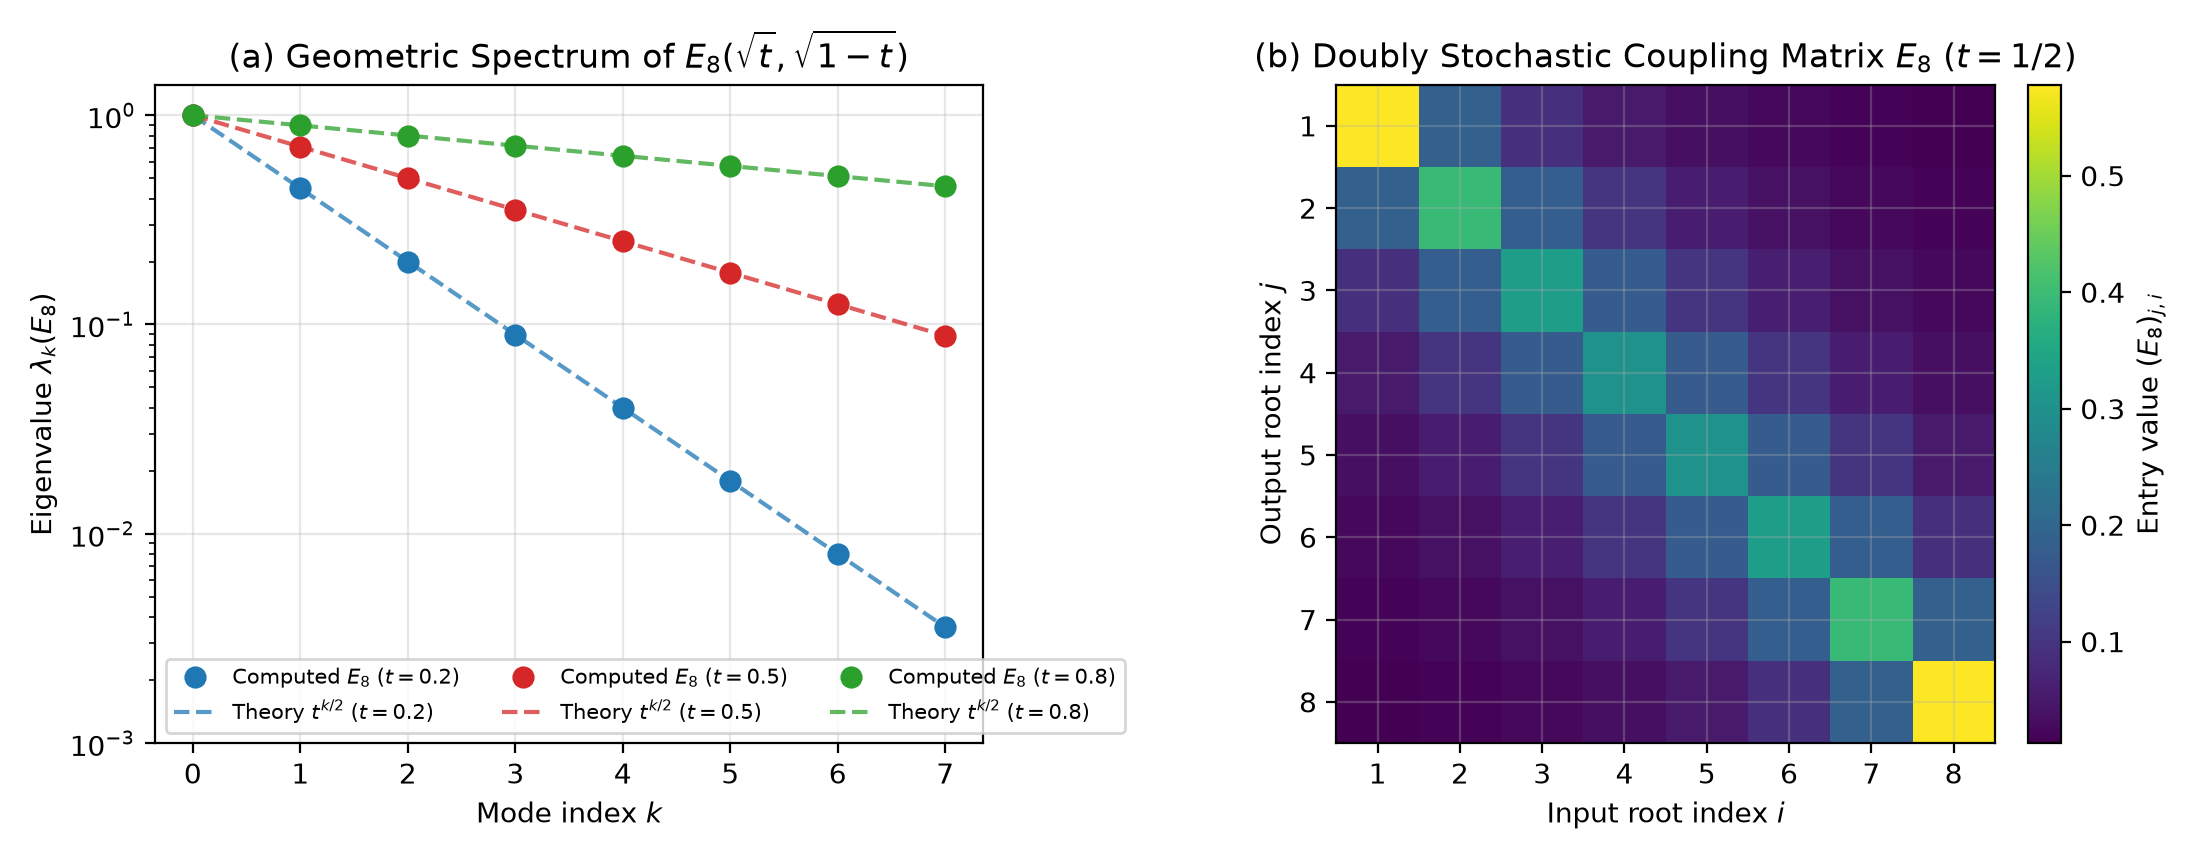
\includegraphics[width=\textwidth]{fig_spectrum_semigroup.png}
\caption{(a) Comparison of computed eigenvalues of $E_8(\sqrt{t},\sqrt{1-t})$ against the exact formula $t^{k/2}$ for $t \in \{0.2, 0.5, 0.8\}$. (b) Entrywise strictly positive, symmetric doubly stochastic coupling matrix $E_8$ at $t=1/2$.}
\label{fig:spec}
\end{figure}

\begin{figure}[htbp]
\centering
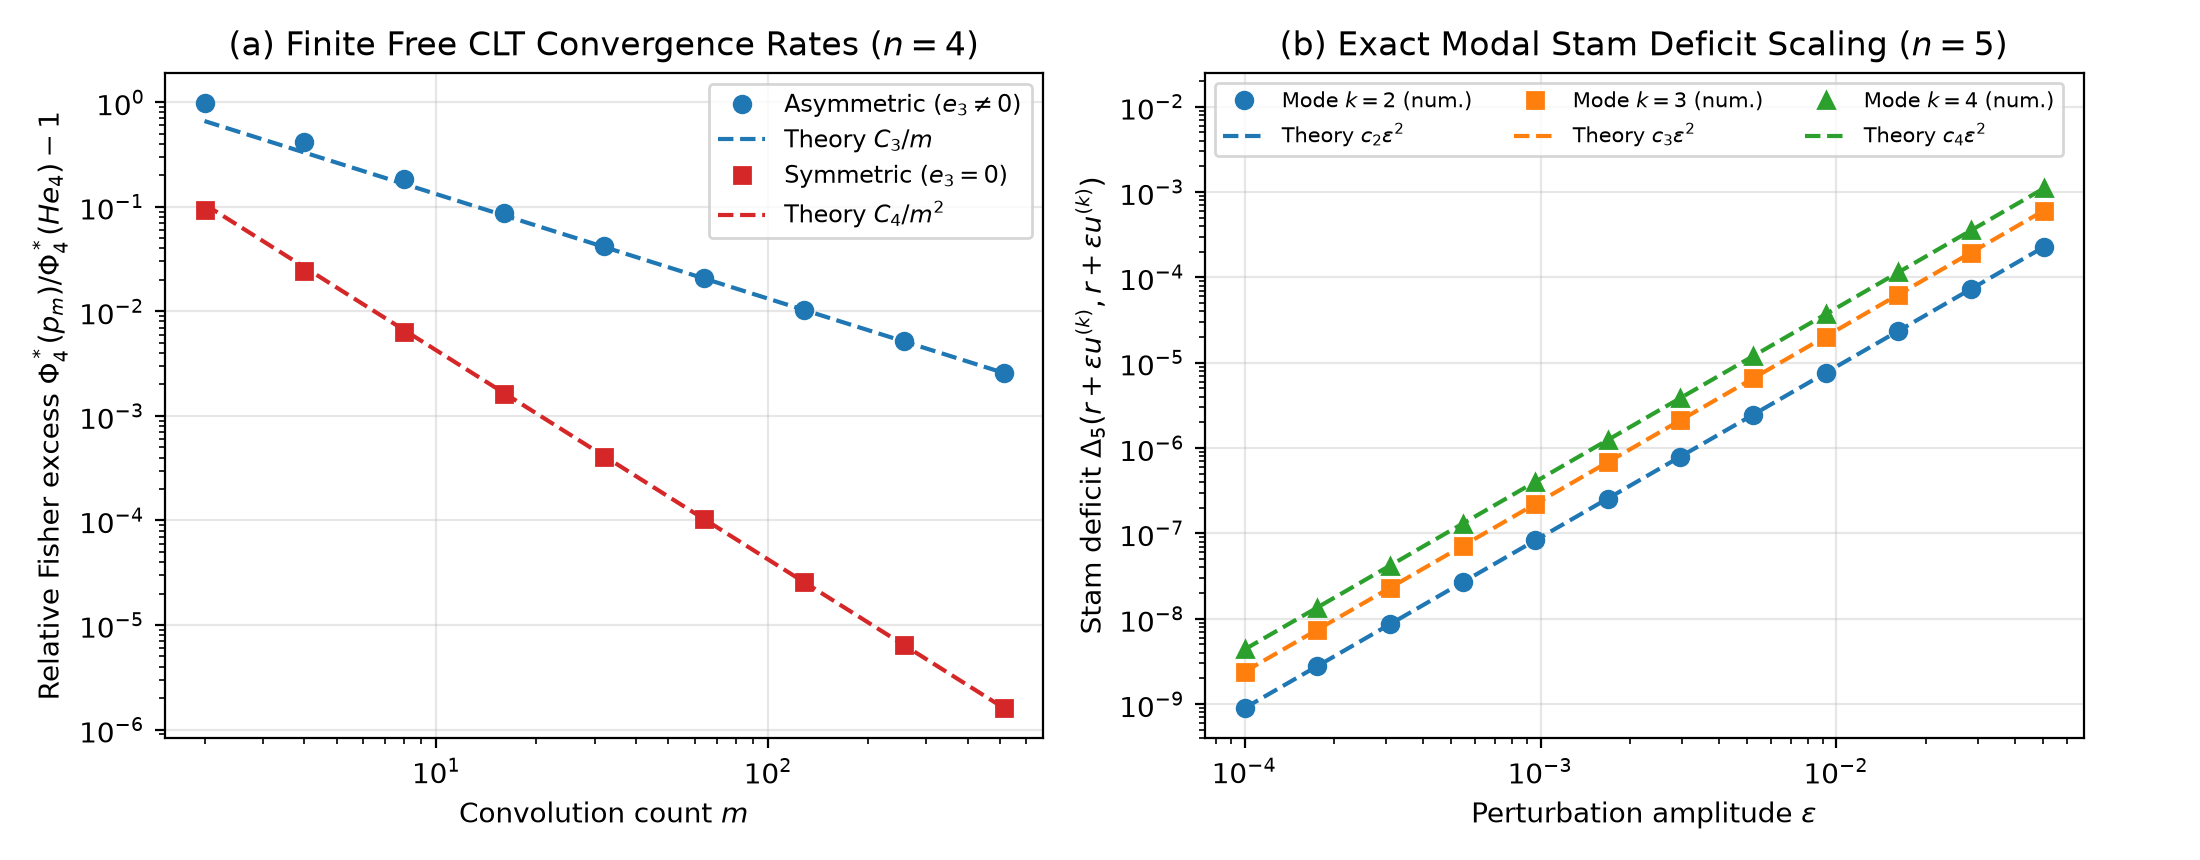
\includegraphics[width=\textwidth]{fig_stam_clt.png}
\caption{(a) Finite free CLT relative Fisher information excess for $n=4$: generic asymmetric polynomials decay as $C_3/m$, while symmetric polynomials ($e_3 = 0$) decay as $C_4/m^2$, matching Theorem~\ref{thm:clt}(b). (b) Quadratic scaling of the Stam deficit along modes $k=2,3,4$ for $n=5$, matching Theorem~\ref{thm:stam-hessian}.}
\label{fig:clt}
\end{figure}

\clearpage
\appendix
\section{Rigorous Interval-Arithmetic Certificates}
\label{app:certificates}

To make the two computer-assisted bounds of Remark~\ref{rem:global-sharpness}(iv) and Remark~\ref{rem:lp-n4-obstruction} completely auditable without relying on floating-point eigenvalues or numerical optimizer output, we record below the exact short integer/rational certificate data and the interval-arithmetic verification protocol implemented in \texttt{verify\_theorems.py} using \texttt{mpmath.iv} at $50$-digit precision.

\subsection*{Protocol for Rigorous Root and Jacobian Enclosures}
Given exact rational root vectors $\alpha, \beta \in \mathbb{Q}^n$, we form the monic convolution polynomial $r(x) := (p_\alpha \boxplusn p_\beta)(x)$ and its derivative $r'(x)$ in interval arithmetic. For each simple real root $\gamma_i$ ($i = 1, \dots, n$), we verify on an explicit isolating bracket $[L_i, U_i]$ (width $2 \times 10^{-35}$, with $U_i < L_{i+1}$) that (i) the upper endpoint of the interval product $r(L_i)\,r(U_i)$ is strictly negative (guaranteeing existence by the intermediate value theorem), and (ii) the interval $r'([L_i, U_i])$ does not contain $0$ (guaranteeing uniqueness and simplicity). Each Jacobian entry is then enclosed directly via the closed-form identity
\[
(J_\alpha)_{i,j} = -\frac{\bigl(\partial_{\alpha_j} p_\alpha \boxplusn p_\beta\bigr)(\gamma_i)}{r'(\gamma_i)} \in -\frac{\bigl(\partial_{\alpha_j} p_\alpha \boxplusn p_\beta\bigr)([L_i, U_i])}{r'([L_i, U_i])},
\]
and analogously for $J_\beta$. Numerical root-finding (\texttt{mp.polyroots}) is used only to propose candidate bracket centers; the proof relies solely on the verified interval sign-change, disjointness, and non-vanishing derivative enclosures, with no floating-point root-finder or eigensolver trusted inside the bound.

\subsection*{Certificate A.1: Rigorous Bound $c_4^{(100)} \le 0.31413321 < \frac{1}{3}$ (Remark~\ref{rem:global-sharpness}(iv))}
Take exact rational base vectors $a_0 := (-1, -\frac{1}{1000}, \frac{1}{1000}, 1)$ and $b_0 := (-3, \frac{999}{1000}, 1, \frac{1001}{1000})$, with exact variance ratio $t := \frac{29}{40} = 0.725$, and set $\alpha := \sqrt{t}\,\|a_0\|_2^{-1} a_0$ and $\beta := \sqrt{1-t}\,\|b_0\|_2^{-1} b_0$ in interval arithmetic. Fix the four-integer test vector
\[
z_0 := (649,\, -512,\, -1000,\, 863)^T \in \mathbb{Z}^4
\]
and project it orthogonally onto $\{\one, \gamma\}^\perp$ in interval arithmetic:
\[
z_1 := z_0 - \frac{\langle z_0, \one\rangle}{4}\,\one, \qquad
z := z_1 - \frac{\langle z_1, \gamma\rangle}{\|\gamma\|_2^2}\,\gamma.
\]
Because $\langle \one, \gamma\rangle = 0$ identically and $\lambda_1\bigl((J_\alpha J_\alpha^T + J_\beta J_\beta^T)|_{\one^\perp}\bigr) = 1$ on $\Span(\gamma)$, the Courant--Fischer theorem gives $\lambda_2\bigl((J_\alpha J_\alpha^T + J_\beta J_\beta^T)|_{\one^\perp}\bigr) \ge (\|J_\alpha^T z\|_2^2 + \|J_\beta^T z\|_2^2)/\|z\|_2^2$. Rigorous interval evaluation yields
\[
\frac{\|J_\alpha^T z\|_2^2 + \|J_\beta^T z\|_2^2}{\|z\|_2^2} \in [0.749478769775,\, 0.749478769776],
\]
and hence
\[
c_4^{(100)} \le \frac{1 - 0.749478769775}{4 \cdot \frac{29}{40} \cdot \frac{11}{40}} < 0.31413321 < \frac{1}{3}.
\]

\subsection*{Certificate A.2: Zero-Residual Dual Proof of $\inf_{u,v \in \R^5} f(u,v) \ge 1.0021479 > 1$ (Remark~\ref{rem:lp-n4-obstruction})}
Take the exact centered rational pair
\[
\alpha_5 := \left(-\frac{128}{125},\, -\frac{251}{250},\, -\frac{123}{125},\, -\frac{241}{250},\, \frac{497}{125}\right), \qquad
\beta_5 := -P\alpha_5,
\]
where $P$ is the $5 \times 5$ reversal permutation matrix. Define the exact rational convex weights
\[
\lambda_1 := \frac{805}{10000}, \qquad \lambda_2 := \frac{7958}{10000}, \qquad \lambda_a = \lambda_b := \frac{1237}{20000}
\]
(satisfying $\lambda_a + \lambda_b + \lambda_1 + \lambda_2 = 1$ identically), together with the disjoint-support left unit vectors
\[
w_1 := \frac{1}{\sqrt{3}}(0, -1, -1, -1, 0)^T, \qquad
w_2 := \frac{1}{\sqrt{2}}(1, 0, 0, 0, -1)^T
\]
and right unit vectors $(x_k, y_k) := (\hat{x}_k, \hat{y}_k) / \|(\hat{x}_k, \hat{y}_k)\|_2 \in \R^{10}$ ($k = 1, 2$) generated from the two-digit integer vectors
\begin{align*}
\hat{x}_1 &:= (-100, -100, -100, -100, 23)^T, & \hat{y}_1 &:= P\hat{x}_1, \\
\hat{x}_2 &:= (30, 30, 29, 29, -100)^T, & \hat{y}_2 &:= -P\hat{x}_2.
\end{align*}
Define $s_a, s_b \in \R^5$ by
\[
s_a := -\frac{\lambda_1(\one^T x_1)\,w_1 + \lambda_2(\one^T x_2)\,w_2}{\lambda_a}, \qquad
s_b := -\frac{\lambda_1(\one^T y_1)\,w_1 + \lambda_2(\one^T y_2)\,w_2}{\lambda_b} = P s_a.
\]
By direct calculation, $\|\hat{x}_1 \oplus \hat{y}_1\|_2^2 = 81058$, $\one^T \hat{x}_1 = -377$, $\|\hat{x}_2 \oplus \hat{y}_2\|_2^2 = 26964$, and $\one^T \hat{x}_2 = 18$. Because $w_1$ and $w_2$ have disjoint supports ($\{2,3,4\}$ vs.\ $\{1,5\}$),
\[
\|s_a\|_\infty = \|s_b\|_\infty
= \max\!\left(\frac{\lambda_1 \cdot 377}{\lambda_a \sqrt{3 \cdot 81058}},\; \frac{\lambda_2 \cdot 18}{\lambda_a \sqrt{2 \cdot 26964}}\right)
< 0.99731 < 1.
\]
Since $s_a, s_b \in [-1, 1]^5$ and all linear terms in $(u, v)$ vanish \emph{identically} ($\lambda_a s_a + \sum_{k=1}^2 \lambda_k (\one^T x_k) w_k = 0$ and $\lambda_b s_b + \sum_{k=1}^2 \lambda_k (\one^T y_k) w_k = 0$), the dual inequality holds globally for every $(u, v) \in \R^5 \times \R^5$ with zero residual:
\[
f(u, v) \ge \lambda_a s_a^T(J_{\alpha_5} e_5) + \lambda_b s_b^T(J_{\beta_5} e_1) + \sum_{k=1}^2 \lambda_k w_k^T\bigl(J_{\alpha_5} x_k + J_{\beta_5} y_k\bigr).
\]
Rigorous interval evaluation over the enclosed Jacobians $J_{\alpha_5}, J_{\beta_5}$ yields the guaranteed enclosure $[1.002147929052,\, 1.002147929053]$, proving $\inf_{u, v \in \R^5} f(u, v) \ge 1.0021479 > 1$.

\clearpage
\section*{Provenance and AI-Assistance Disclosure}

This manuscript was developed through a human-directed, multi-agent AI research workflow. AI systems were used extensively for exploratory calculations, proof generation and drafting, literature cross-checking against primary arXiv LaTeX sources, multi-round adversarial review, and implementation of the companion verification script \texttt{verify\_theorems.py}.

To keep epistemic status and provenance transparent:
\begin{itemize}
\item The theorems and propositions in Sections~2--6 are presented as analytical proofs checked symbolically/numerically and across multiple independent AI review rounds, but they have \emph{not yet been verified line-by-line by a human specialist in finite free probability}.
\item The quartic Fisher-information bound of Remark~\ref{rem:global-sharpness}(i) is verified in exact rational arithmetic ($\mathbb{Q}$).
\item The degree-$4$ eq.~(100) bound (Remark~\ref{rem:global-sharpness}(iv)) and degree-$5$ linear-extension obstruction (Remark~\ref{rem:lp-n4-obstruction}) are verified in $50$-digit rigorous interval arithmetic (\texttt{mpmath.iv}) using the short explicit integer/rational certificate data printed in Appendix~\ref{app:certificates}.
\item The remaining optimization entries in Table~\ref{tab:verif} are exploratory numerical evidence.
\end{itemize}

Tristan Schubert (a university student working in the field of AI who directed the workflow, problem selection, adversarial audit process, and verification pipeline) takes responsibility for the accurate reporting of the methodology and AI provenance, the fidelity of citations to their primary sources, the reproducibility of the accompanying code and interval certificates, and for issuing corrections or withdrawals if errors are identified. Because the deeper analytical arguments lie outside his specialist mathematical training, this document is shared transparently as an AI-assisted working draft rather than a human-certified pure-mathematics submission, and independent review, critique, or collaboration by specialists in finite free probability is warmly welcomed.

\begin{thebibliography}{9}

\bibitem{AP2018}
O.~Arizmendi and D.~Perales,
\emph{Cumulants for finite free convolution},
J. Combin. Theory Ser. A \textbf{155} (2018), 244--266, arXiv:1611.06598.

\bibitem{AP2020}
O.~Arizmendi and D.~Perales,
\emph{A Berry--Esseen type theorem for finite free convolution},
in \emph{XIII Symposium on Probability and Stochastic Processes},
Progress in Probability, vol.~\textbf{75}, Birkh\"auser/Springer, Cham, 2020, pp.~67--76.

\bibitem{GSS2026}
J.~Garza-Vargas, N.~Srivastava, and Z.~Stier,
\emph{Finite Free Information Inequalities},
arXiv:2602.15822 [math.PR], 2026.

\bibitem{Hashemi2026}
B.~Hashemi,
\emph{Spectral Structure in Finite Free Information Inequalities and $p$-Stam Phase Transitions},
arXiv:2604.11922 [math.PR], 2026.

\bibitem{HH2026}
B.~Hashemi and J.~Hyun,
\emph{When Finite Free Curves Split},
arXiv:2609.10367 [math.AG], 2026.

\bibitem{MSS2022}
A.~W.~Marcus, D.~A.~Spielman, and N.~Srivastava,
\emph{Finite free convolutions of polynomials},
Probab. Theory Related Fields \textbf{182} (2022), 807--848, arXiv:1504.00350.

\bibitem{Sasaki15}
R.~Sasaki,
\emph{Perturbations around the zeros of classical orthogonal polynomials},
J. Math. Phys. \textbf{56} (2015), 042106.

\end{thebibliography}

\end{document}
